%%%%%%%%%%%%%%%%%%%%%%%%%%%%%%%%%%%%%%%%%%%%%%%%%%%%%%%%%%%%%%%%%%%%%%%%%%%%%%%
% Descripción: Template para la generación de la tesis de la MDIAE
% Autor: 
% Fecha: 20/05/2016
%%%%%%%%%%%%%%%%%%%%%%%%%%%%%%%%%%%%%%%%%%%%%%%%%%%%%%%%%%%%%%%%%%%%%%%%%%%%%%%

%%%%%%%%%%%%%%%%%%%%%%%%%%%%%%%%%%%%%%%%%%%%%%%%%%%%%%%%%%%%%%%%%%%%%%%%%%%%%%%
%%	PARA INSERTAR FIGURAS USAR LA FUNCION PREDEFINIDA \imagen
%%
%%      \imagen{escala}{path imagen}{caption}{referencia}
%%
%% donde:
%% 	* escala: es un valor numérico. Preferentemente usar valores entre 0 y 1.
%%		(ejemplo: 0.2)
%% 	* path: imagen es el directorio relativo donde se encuentra la imagen
%%		(ejemplo: Figures/Logos/conae-logo.png)
%%	* caption: texto de pie de figura.
%%	* referencia: texto que sirve para citar la figura. 
%%		(ejemplo: fig:conaelogo) luego se podrá hacer referencia \ref{fig:conaelogo}
%%%%%%%%%%%%%%%%%%%%%%%%%%%%%%%%%%%%%%%%%%%%%%%%%%%%%%%%%%%%%%%%%%%%%%%%%%%%%%%

%------------------------------------------------------------------------------
% Formato del documento
\documentclass[11pt, a4paper, twoside]{report}

%------------------------------------------------------------------------------
% TEMPLATE MDIAE (ACÁ SE ENCUETRAN LAS CUSTOMIZACIONES)
% Remitirse al archivo mdiaedoc.sty
\usepackage{mdiaedoc}

%Configuración de los márgenes
\usepackage[top=3cm, bottom=3cm, left=2.5cm, right=1.5cm]{geometry}


%------------------------------------------------------------------------------
% Esto no se usa (YA ESTA DEFINIDO EN EL TEMPLATE)
%\usepackage{setspace}

%%%%%%%%%%%%%%%%%%%%%%%%%%%%%%%%%%%%%%%%%%%%%%%%%%%%%%%%%%%%%%%%%%%%%%%%%%%%%%%
% COMIENZO DEL DOCUMENTO
%%%%%%%%%%%%%%%%%%%%%%%%%%%%%%%%%%%%%%%%%%%%%%%%%%%%%%%%%%%%%%%%%%%%%%%%%%%%%%%
\begin{document}

\makeatletter
\author{M. Cecilia Valenti}
\makeatother

%------------------------------------------------------------------------------
% PORTADA
\portadatesis{ARxCODE\\Prototipo de software para el An\'alisis de Riesgo por Colisi\'on con Desechos Espaciales.}{M. Cecilia Valenti.}{UNIVERSIDAD NACIONAL DE LA MATANZA}{Mayo, 2017}{2017}{Marcelo Colazo}{CONAE, Córdoba, Argentina}%{}{}

%------------------------------------------------------------------------------
% EN CASO DE TENER UN ASESOR CIENTIFICO, DESCOMENTAR LO SIGUIENTE 
% \begin{center}
% \normalsize ASESOR CIENTÍFICO:\\
% \normalsize \textit{\textbf{Nombre del asesor}}\\
% \end{center}

%------------------------------------------------------------------------------
% COMPLETAR CON LICENCIA CREATIVE COMMONS SEGÚN CORRESPONDA
%\begin{center}
%%%%% Ejemplo %%%%%%
%\begin{figure}[H]
%    \centering
%    
\includegraphics[width=3cm, keepaspectratio=true]{imagenes/Logos/creativecommons.png}
%\end{figure}
%\vspace*{-0.5cm}
%Esta obra está bajo una \href{http://creativecommons.org/licenses/by-sa/2.5/ar/}{Licencia Creative Commons Atribución-CompartirIgual 2.5 Argentina.}
%\end{center}

\pagenumbering{gobble}

\chapter*{Abstract}
\label{chap:abstract}

\textbf{Keywords:}
\chapter*{Resumen}
\label{chap:resumen}
En este trabajo presentamos el prototipo de software ARxCODE. Un sistema dise\~nado para el estudio de acercamientos con riesgo de colisi\'on, entre misiones satelitales operativas y desechos espaciales.\\

ARxCODE tiene la capacidad de extraer la informaci\'on que proviene de los mensajes de alerta de colisiones estandarizados, CDM (Conjunction Data Message), definidos por el CCSDS (Consultative Committee for Space Data System) y de procesar datos ingresados manualmente.\\
Devuelve al operador par\'ametros para el an\'alisis de riesgo como: la m\'inima distancia y la probabilidad de colisi\'on en una interfaz gr\'afica que facilita una clara caracterizaci\'on y visualizaci\'on de la situaci\'on.\\

Los estudios de acercamientos de riesgo que involucran desechos espaciales acarrean grandes incertezas respecto a la posici\'on del desecho, en especial para aquellos organismos que no cuentan con instrumentos propios de rastreo.\\

En la actualidad, adem\'as de la distancia m\'inima de acercamiento, debe considerarse la probabilidad de colisi\'on. El c\'alculo de la probabilidad de colisi\'on requiere tener conocimiento de los errores de las posiciones y esto no siempre es conocido, en particular para los desechos, cuyos TLE son p\'ublicos, pero no sus errores asociados.\\

Para la construcci\'on de la matriz de covarianza de la posici\'on del desecho correspondiente al \'ultimo TLE disponible m\'as cercano al momento del m\'aximo acercamiento (TCA: Time of Closest Approach), se implementa el m\'etodo desarrollado por Osweiler.\\

Para la estimaci\'on de los errores que introducen las propagaciones de los TLE (Two-Line Elements) con el modelo de propagaci\'on anal\'itico SGP4 (Simplified General Perturbations) desarrollamos una metodolog\'ia que incorpora el análisis hist\'orico de los productos orbitales precisos de la misi\'on SAC-D.\\

Finalmente para el c\'alculo de la probabilidad de colisi\'on, se implementa un m\'etodo simplificado desarrollado por Lei-Chen.\\
ARxCODE es una herramienta que ofrece a los operadores de los centros de control de misi\'on, la posibilidad de tener una visi\'on m\'as clara de las situaciones de encuentro, para aquellos momentos de intercambio de di\'alogo con los organismos internacionales de alerta.

\textbf{Palabras clave:}:space debris --- collision avoidance --- probability of collision
\endinput
%%%% Texto (no menos de 200 palabras)


La capacidad de predecir y evitar el riesgo de colisión de un sat\'elite operativo con un desecho espacial, se ve limitada por los errores de precisi\'on con los que se conocen las \'orbitas de los desechos espaciales.\\

En la actualidad s\'olo EE.UU y Rusia, y la comunidad europea dando sus primeros pasos, cuentan con redes e instrumentos de rastreo que les permiten confeccionar bases de datos con la informaci\'on orbital de los objetos que rodean la Tierra.\\

En este contexto, las maniobras que involucren a las misiones de la Comisi\'on Nacional de Actividades Espaciales (CONAE) con riesgo de colisi\'on, se planifican a partir de la informaci\'on que le proveen servicios externos a trav\'es de convenios con alto grado de confidencialidad e informaci\'on restringida.\\ 

Organismos como el \ac{JSpOC} de EE.UU, tienen la capacidad de predecir encuentros y los notifica con una antelaci\'on de 72 horas, a trav\'es de sus mensajes de alerta: \ac{CDM} \cite{CDM}.\\
Estos mensajes proveen informaci\'on de los objetos involucrados en el encuentro, las posiciones y velocidades de ambos, el instante predicho para el encuentro, \ac{TCA} y las matrices de error para el TCA.\\

\textcolor{red}{A partir de los datos que ofrece el \ac{CDM}, nos proponemos desarrollar una t\'ecnica que mejore la estimaci\'on de la posici\'on del desecho espacial, e incorpore los datos orbitales que el departamento de Din\'amica Orbital ofrece en el c\'alculo de la \ac{PoC}, para contar con una mejor caracterizaci\'on de la situaci\'on al momento del intercambio de informaci\'on con los organismos y servicios externos.}\\

\chapter*{Agradecimientos}
\label{chap:agradecimientos}

En primer lugar, agradezco a mi director Marcelo Colazo, que dirigi\'o este trabajo y desde hace ya varios a\~nos me acompa\~na y me ayuda en las distintas oportunidades que van surgiendo para mi desarrollo profesional. 

Agradezco tambi\'en a Alicia Mon, mi codirectora y a los jurados: Jos\'e L. Roca, Walkiria Schulz y Livio Gratton por su tiempo y dedicaci\'on en la revisi\'on detallada del trabajo. 

Al director del Instituto M. Gulich, Leonardo De Ferraris, al director de la MDIAE Carlos Barrientos, al Dr. Jorge Ierache y a todas las autoridades, docentes y personal administrativo tanto de la UFS de CONAE como de la UNLaM, que trabajaron para hacer posible esta maestr\'ia.\\


A t\'itulo personal, agradezco a mis compa\~neros de cursada y los amigos que estuvieron cerca en esta etapa. Agradezco profundamente a mi familia por el apoyo incondicional siempre y a Soligo, mi compa\~nero de mates y de vida.\\


Por \'ultimo, agradezco a todo el pueblo argentino que ha financiado mi formaci\'on de grado en la universidad pública de La Plata y esta maestr\'ia entre la universidad p\'ublica de la Matanza y la CONAE. 





 %% OPCIONAL

\tabladecontenidos

\chapter*{Lista de acrónimos}
\label{chap:acronimos}

\begin{acronym}[ARxCODE]
\acro{CONAE}{Comisi\'on Nacional de Actividades Espaciales}
\acro{ARxCODE}{An\'alisis de Riesgo por Colisi'on con Desechos Espaciales}
\acro{CDM}{Conjunction Data Message}
\acro{TLE}{Two-Line elements}
\acro{SGP4}{Simplified General Perturbations model}
\acro{JSpOC}{Joint Space Operations Center}
\acro{NORAD}{North American Aerospace Defense Command}
\acro{PoC}{Probabilidad de Colisi\'on}
\acro{TCA}{Time of Closest Approach}
\acro{ESA}{European Space Agency}
\acro{NASA}{National Aeronautics and Space Administration}
\acro{ISS}{International Space Station}
\acro{RMM}{Risk Mitigation Maneuver}
\acro{COPUOS}{Committee of the Peacefull Uses of Outer Space (ONU)}
\acro{IADC}{Inter-Agency Space Debris Coordination Commitee}
\acro{CCSDS}{Consultative Committee for Space Data Systems}
\acro{LEO}{Low Earth Orbit}
\acro{GEO}{Geostationary Orbit}
\acro{ONU}{Organizaci\'on de las Naciones Unidas}
\acro{SI}{Sistema Internacional de Unidades}
\acro{TOD}{True of Date}
\acro{TEME}{True Equator Mean Equinox}
\acro{ECI}{Earth Centered Inercial}
\acro{RTN}{Radial, Transverse, Normal}
\acro{IDE}{Integrated Development Environment}
\acro{CODS}{CONAE Orbyt Dynamics Services}
\end{acronym}



%------------------------------------------------------------------------------
% Numeración arábiga a partir de este punto
\pagenumbering{arabic}
\setcounter{page}{1}

\chapter{Introducción}
\label{chap:introduccion}


\section{Los desechos espaciales}

El comienzo de la era satelital en el a\~no 1957 con la puesta en \'orbita del sat\'elite ruso Sputnik signific\'o la conquista de un nuevo espacio y un cambio de paradigma en lo que respecta a las tecnolog\'ias para las comunicaciones, los estudios de nuestro planeta, el sistema solar, las formas de navegar, de geoposicionarse y el intercambio de informaci\'on. Desde entonces el ambiente espacial cada vez suma m\'as colonos (Fig. \ref{fig:cantidad2014}).\\

Las experiencias de las primeras misiones aportaron mucho conocimiento de este entorno con caracter\'isticas muy distintas a las de la superficie de la Tierra y permitieron ir mejorando las t\'ecnicas y los materiales para que los sat\'elites cumplieran sus objetivos sin mayores inconvenientes.
Sin embargo, un hecho poco predicho o abordado empez\'o a ocupar prioridad en las dos \'ultimas d\'ecadas: los {\it{desechos espaciales}}.\\

{\bf{Definici\'on:}}{\it{ Son Desechos Espaciales todos los objetos construidos por el hombre, incluyendo fragmentos o partes de los mismos, que orbitan la Tierra o reingresan a la atm\'osfera y no son funcionales, es decir, han perdido su capacidad operativa.}} \citep{iadcguide}\\

La disponibilidad del espacio parec\'ia ilimitada, y los primeros a\~nos no se ten\'ian consideraciones respecto a los objetos que all\'i se depositaban, o se desprend\'ian de los cohetes y las misiones. Pero con el correr del tiempo, ciertas regiones del espacio cobraron inter\' es estrat\'egico, y la superpoblaci\'on en dichas zonas no tard\'o en mostrar complicaciones.\\

Los desechos representan hoy el mayor porcentaje de los objetos que orbitan la Tierra y los estudios de su proliferaci\'on, indican que, de no existir planes de acci\'on para subsanar la situaci\'on, el efecto de las colisiones en cascada transformar\'a el ambiente espacial en un lugar inhabitable para cualquier misi\'on.\\

La primera colisi\'on confirmada y claramente registrada entre una misi\'on operativa y un desecho, ocurri\'o el 24 de Julio de 1996, cuando el sat\'elite franc\'es Cerise (95-033B) fue embestido por un fragmento (86-019RF), remanente de la explosi\'on de la \'ultima etapa del cohete Ariane-1 H-10, ocurrida el 13 de noviembre de 1986; nueve meses despu\'es de inyectar en \'orbita al sat\'elite SPOT-1. La reconstrucci\'on de la situaci\'on luego de la colisi\'on, coincide plenamente con una p\'erdida de la actitud del Cerise que fue registrada en los datos hist\'oricos abordo \citep{KlinkradChapter8}.\\

%Este accidente fue un disparador en lo que respecta al estudio de los desechos espaciales y las colisiones. (correcion walkiria)
Las estad\'isticas de la base de datos de Scopus \footnote{https://www.scopus.com/}, indican que las investigaciones respecto a la tem\'atica de desechos espaciales en general muestran un continuo crecimiento (Fig. \ref{fig:scopusSD}). Resultados similares se obtienen respecto de la tem\'atica de colisiones (Fig. \ref{fig:scopusCA}); si bien no se ha podido hacer una vinculaci\'on directa entre sucesos, picos y tendencias, se mencionan algunos eventos que podr\'ian estar relacionados con los resultados. En el a\~no 1988 la \ac{NASA} implementa su sistema para analizar y evitar colisiones en las misiones tripuladas ({\it{Collision Assessment and Collision Avoidance System}}), a continuaci\'on en el a\~no 1990 se lanza el telescopio espacial {\it{Hubble Space Telescope}} y se realiza un congreso de gran trascendencia, el {\it{Orbital Debris Conference: Technical Issues and Future Directions }}. Se observa un pico a partir del a\~no 1998, probablemente vinculado al lanzamiento de la estaci\'on espacial internacional o \ac{ISS}, y luego un notorio crecimiento a partir del a\~no 2007, vinculado a dos sucesos: la destrucci\'on intencional de China de uno de sus sat\'elites en una prueba misil\'istica y la colisi\'on catastr\'ofica accidental entre el sat\'elite ruso KOSMOS 2251, fuera de servicio y el sat\'elite IRIDIUM 33, operativo, de la constelaci\'on de IRIDIUM, en el a\~no 2009.\\

%La misma tendencia puede verse en la tem\'atica de colisiones (Fig. \ref{fig:scopusCA}), destac\'andose el gran escal\'on a partir del a\~no 1993 (colisi\'on del sat\'elite Cerise),



\begin{figure}[!h]
\centering
  \textbf{Publicaciones sobre Desechos Espaciales (Scopus)}\par\medskip
    \fbox{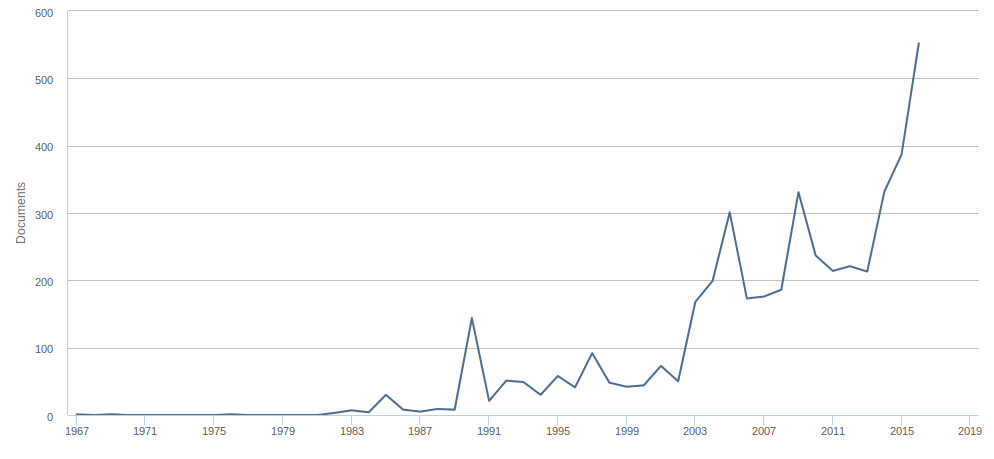
\includegraphics[width=0.8\columnwidth, keepaspectratio]{imagenes/scopusSD}}
    \caption[Desechos Espaciales seg\'un Scopus]{Estad\'istica de las investigaciones realizadas en el \'area de desechos espaciales ({\it{Space Debris}}) de acuerdo a la base de datos de Scopus.}
    \label{fig:scopusSD}
\end{figure}

\begin{figure}[!h]
\centering
   \textbf{Publicaciones sobre Colisiones (Scopus)}\par\medskip
    \fbox{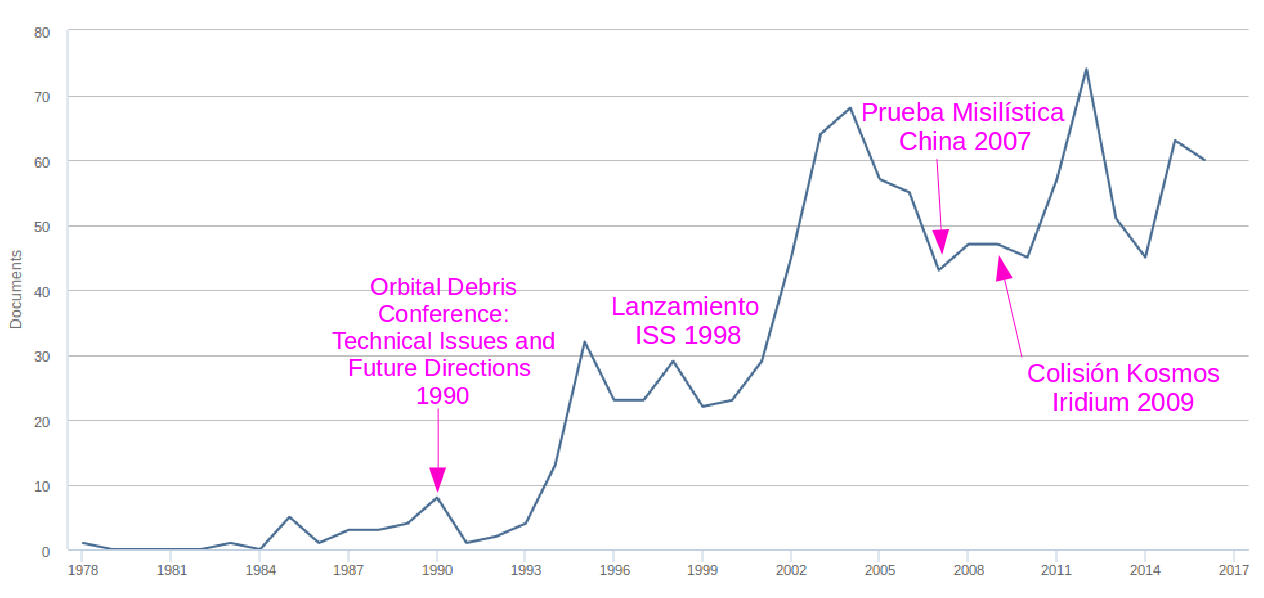
\includegraphics[width=0.7\columnwidth, keepaspectratio]{imagenes/scopusCA}}
    \caption[Riesgos de Colisi\'on seg\'un Scopus]{Estad\'istica de las investigaciones realizadas en el \'area de riesgos de colisi\'on {\it{Collision Avoidance}} de acuerdo a la base de datos de Scopus.}
    \label{fig:scopusCA}
\end{figure} 

\subsection*{Distintos abordajes para el estudio de los desechos espaciales}
Existen distintos estudios respecto a la problem\'atica de los desechos espaciales. La \ac{NASA} propone una clasificaci\'on general seg\'un sean estudios de: modelado, rastreo, protecci\'on, mitigaci\'on, reparaci\'on o reingreso.\\
\begin{itemize}
%\setlength{\itemsep}{0pt}
\item {\bf{Modelado:}} Consiste en el desarrollo y la actualizaci\'on de los modelos orbitales de los desechos, para describir y caracterizar el ambiente actual y la proyecci\'on futura.\\
\item {\bf{Rastreo:}} Mediciones que se hacen con radares y telescopios \'opticos desde tierra, y tambi\'en con telescopios espaciales.\\
\item {\bf{Protecci\'on:}} Estudios hechos en impactos de alta velocidad para el desarrollo de nuevos materiales y dise\~nos que ofrezcan una mayor protecci\'on.\\
\item {\bf{Mitigaci\'on:}} Planifiaci\'on de estrategias para reducir la generaci\'on de nuevos desechos. Generaci\'on de documentaci\'on  de buenas pr\'acticas, est\'andares y promoci\'on de acuerdos internacionales.\\
\item {\bf{Reparaci\'on:}} Dise\~no de misiones con el \'unico objetivo de actuar sobre los desechos a fin de reducir el n\'umero de objetos inactivos en \'orbita.\\
\item {\bf{Reingreso:}} Identificaci\'on de los reingresos no controlados, para hacer an\'alisis sobre las zonas de posibles impactos en Tierra y la planificaci\'on de reingresos controlados.\\
\end{itemize}

Organismos como el Centro Principal de Inteligencia Espacial Ruso, el Departamento de Defensa Norteamericano, la NASA y la \ac{ESA}, han desarrollado tanto modelos de evoluci\'on como de ingenier\'ia, y mantienen cat\'alogos actualizados con las trayectorias de aquellos objetos cuyo tama\~no permite detectarlos con instrumentos de rastreo en Tierra.\\

Los modelos de evoluci\'on muestran la configuraci\'on actual y proyecciones de configuraciones futuras del ambiente espacial incluyendo todos los objetos que orbitan la Tierra.\\

Los modelos de ingenier\'ia se enfocan en distintas pruebas de laboratorio o de misiones espec\'ificas en \'orbita, que analizan la respuesta de los materiales cuando se exponen a impactos con fragmentos de distinto tipo, particularmente en aquellos de tama\~nos muy chicos pero que colisionan a velocidades del orden de diez kil\'ometros por segundo.\\

En este trabajo nos enfocamos en el an\'alisis de las situaciones de riesgo de colisi\'on, dentro del marco de la {\it{mitigaci\'on}}, para las misiones y los desechos que se ubican en las  \ac{LEO}, u \'orbitas bajas.\\

\subsection*{El entorno de los desechos espaciales: presente y futuro}
Seg\'un los informes de la \ac{ESA} \citep{esaSD}, desde 1957 hasta la actualidad, 5250 lanzamientos han poblado el ambiente espacial con casi 23000 objetos de los cuales, s\'olo cerca de 1200 son sat\'elites operativos.\\

El \ac{IADC}, clasifica los desechos seg\'un sean: objetos relacionados a alguna misi\'on, fragmentos, o cohetes y objetos que ya finalizaron su misi\'on (Tabla \ref{tab:desechosIADC}).\\

\begin{table}[!h]
\caption[Clasificaci\'on de Desechos seg\'un la IADC]{Clasificaci\'on de desechos, causas y recomendaciones del IADC}
\resizebox{17.5cm}{!}{
\begin{tabular}[c]{cll}
\hline 
\rowcolor{lightgray}
\bf{Clasificaci\'on}  &    \bf{Causas} & \bf{Recomendaciones del IADC}\\
\hline
\multirow{ 2}{*}{Objetos relacionados a una misi\'on} &   Liberados intencionalmente& Dise\~nos que reduzcan la liberaci\'on de desechos\\
&Liberados sin intenci\'on& Dise\~nos robustos\\
\hline
\multirow{ 4}{*}{Fragmentos}& Destrucci\'on intencional & Evitar destrucciones intencionales.\\
& Fragmentaciones durante las operaciones & Aseguramiento de la misi\'on.\\
& Fragmentaciones ya finalizada la misi\'on & Reducci\'on de estas situaciones en el dise\~no.\\
& \cellcolor{blue!25}{Colisiones en \'orbita} & Planificaci\'on de maniobras evasivas por riesgo\\
&&de colisi\'on. Protecci\'on.\\
\hline
Objetos que ya finalizaron & Maniobras de disposal inadecuadas &Maniobras de reingreso\\
su misi\'on y cohetes && \\
\hline
\end{tabular} }
\label{tab:desechosIADC}
\begin{flushleft}
\small {\it{Nota.}} Adaptado de la gu\'ia de recomendaciones del IADC, \citep{iadcguide}.
\end{flushleft}
\end{table}


De a acuerdo a una publicaci\'on de la NASA, \citep{ODQNum}, hasta el 04 de Abril de 2017, se contabilizaron $18347$ objetos catalogados (Tabla \ref{tab:objpais}). Clasificados seg\'un sean: cargas \'utiles ({\it{payloads}}), cohetes ({\it{rocket bodies}}), desechos de misi\'on ({\it{mission-related bodies}}), desechos an\'omalos ({\it{anomalous debris}}) o desechos de fragmentaci\'on ({\it{breakup debris}}); ver Figura \ref{fig:catxtipo}.\\

\begin{table}
 \caption[Objetos en \'Orbita al 4 de Abril de 2017.]{Objetos en \'Orbita al 4 de Abril de 2017.}
 \begin{tabular}{lccc}
  \hline 
  \rowcolor{lightgray}
  \bf{Pa\'is}  &    \bf{Cargas \'Utiles} & \bf{Cohetes y Desechos} & TOTAL\\
  \hline 
  China & 235 & 3566&3801\\
  Comunidad de Estados Independientes & 1508&4993&6501\\
  Agencia Espacial Europea &74&60&134\\
  Francia & 62&470&532\\
  India & 79 & 113 & 192\\
  Jap\'on & 162 & 94 & 256\\
  Estados Unidos de Am\'erica & 1513 & 4504 & 6017\\
  Otros & 801 & 113 & 914 \\
  \hline
  \rowcolor{lightgray}
  TOTAL & 4434 & 13913 & 18347 \\
  \hline
 \end{tabular}
 \label{tab:objpais}
 \begin{flushleft}
\small {\it{Nota.}}  Adaptado de NASA, \citep{ODQN}.
\end{flushleft}
\end{table}

\begin{figure}[!h]
\centering
    \fbox{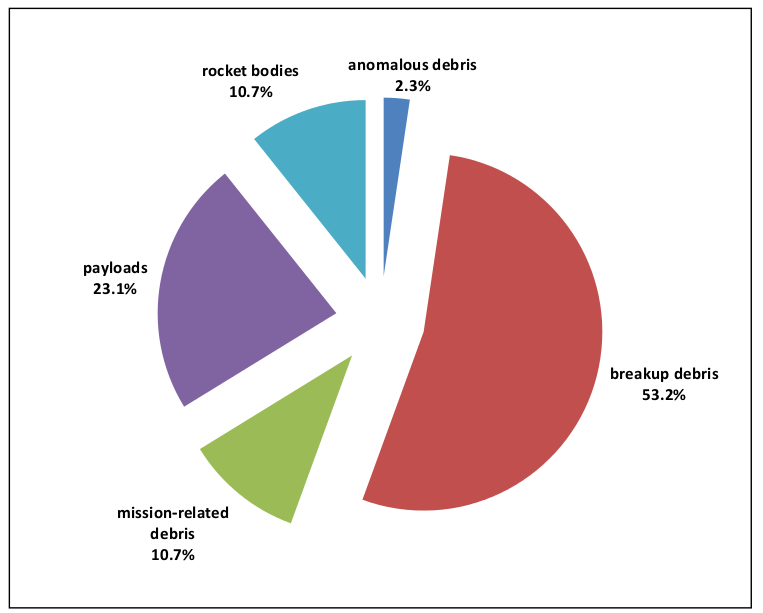
\includegraphics[width=0.7\columnwidth, keepaspectratio]{imagenes/clasificacion2016}}
    \caption[Objetos en \'Orbita seg\'un NASA.]{Porcentaje de Objetos en \'Orbita seg\'un la clasificaci\'on de NASA. Extra\'ido de NASA, \citep{ODQN}.}
    \label{fig:catxtipo}
\end{figure}

Otra clasificaci\'on podr\'ia ser en funci\'on de la distancia a la superficie de la Tierra, ya que la distribuci\'on no es homog\'enea. La relaci\'on entre la densidad de objetos y la altura a la que se encuentran, señala que existen regiones m\'as comprometidas.
Las \'orbitas bajas o \ac{LEO} con un rango de alturas entre los 500 y los 2000 kil\'ometros, son las m\'as superpobladas y contienen casi el 70 \% de todos los objetos catalogados. 
Cabe destacar que en esta regi\'on se ubican las misiones de la serie SAC de la CONAE, las misiones futuras SAOCOM Y SABIAMAR. Ver Figura \ref{fig:Dvsaltura}.\\

\begin{figure}[!h]
  \centering
  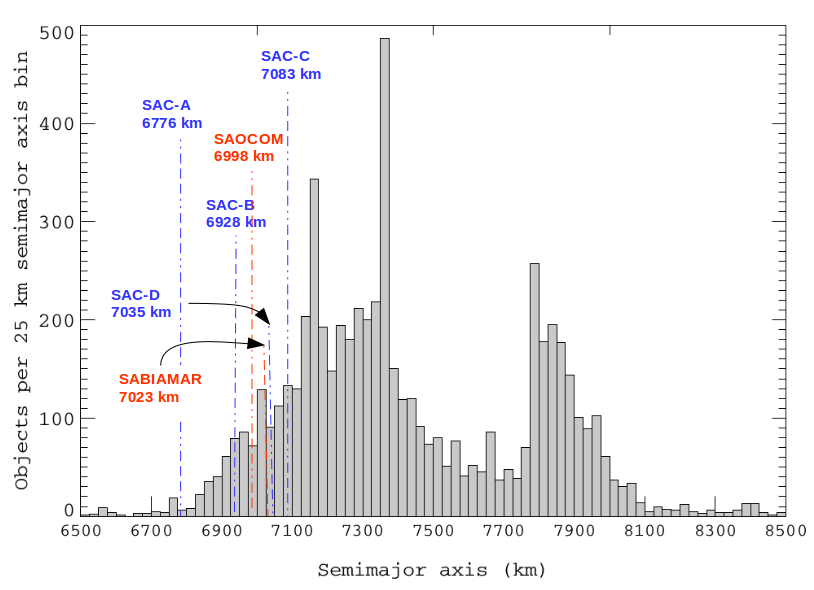
\includegraphics[width=0.9\textwidth]{imagenes/SDvsaltura2011CONAE}
  \caption[Distribuci\'on de objetos en funci\'on del semieje mayor.]{Distribuci\'on de objetos en funci\'on del semieje mayor en la regi\'on LEO. Adapatado de \citep{Klinkrad}. Se agregan en color azul las posiciones de las misiones de CONAE ya puestas en \'orbita (serie SAC) y en color naranja las posiciones de las futuras misiones SAOCOM y SABIAMAR}
  \label{fig:Dvsaltura}
\end{figure}

Si se mira hacia el futuro, las predicciones no son alentadoras. Si bien, los acuerdos internacionales en relaci\'on a acciones para reducir la proliferaci\'on de desechos avanzan y muestran buenos resultados, los proyectos de nuevas misiones tienden a aumentar el n\'umero de objetos, sobre todo en las \'orbitas bajas. Para estas \'orbitas las colisiones pasar\'ian a ser las principales generadoras de desechos.\\

En un reporte t\'ecnico publicado por la NASA \citep{karacalioglu2016impact}, se eval\'uan las nuevas tendencias de la industria satelital y se analiza el futuro panorama del entorno espacial en las \'orbitas bajas, en funci\'on de los lanzamientos planificados y las misiones anunciadas, (Fig. \ref{fig:satxlanz}).\\

En los \'ultimos a\~nos se ha incrementado el n\'umero de agencias o empresas que se dedican al desarrollo espacial. El nuevo paradigma de constelaciones de peque\~nos sat\'elites, sistemas distribuidos o arquitecturas fragmentadas en reemplazo de los grandes y costosos sat\'elites tradicionales, ha permitido la democratizaci\'on del espacio, facilit\'andole el acceso a m\'as agencias y empresas. 
Un claro ejemplo son las constelaciones para comunicaciones anunciadas por OneWeb y SpaceX, que proyectan lanzar del orden de 600 sat\'elites cada una para fines del 2019.

\begin{figure}[!h]
  \centering
  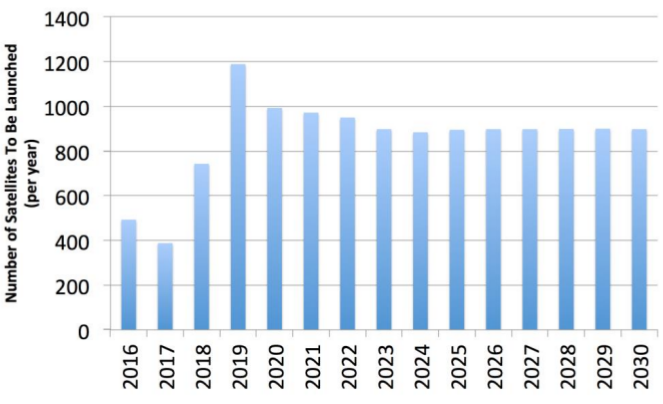
\includegraphics[width=0.7\textwidth]{imagenes/satelxlanz}
  \caption[Proyecci\'on de Sat\'elites 2016-2030]{Proyecci\'on de Sat\'elites 2016-2030. Extra\'ido de \citep{karacalioglu2016impact}}
  \label{fig:satxlanz}
\end{figure}

Estas futuras misiones, no s\'olo generan un aumento en la poblaci\'on espacial durante su vida \'util, sino que, una vez finalizada la misi\'on es importante definir acciones que remuevan esos objetos de la regi\'on de LEO; ya que dependiendo de sus caracter\'isticas, pueden permanecer en \'orbita inactivos por m\'as de 20 a\~nos.\\

A su vez, aunque ya existen modelos experimentales y en desarrollo en lo que respecta a recuperar partes de los lanzadores, cada lanzamiento inyecta en \'orbita no s\'olo los sat\'elites sino tambi\'en las \'ultimas etapas de los cohetes lanzadores, (Fig. \ref{fig:rocketbodies}).\\

\begin{figure}[!h]
  \centering
  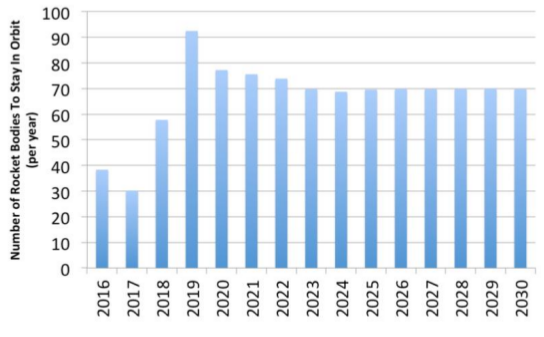
\includegraphics[width=0.7\textwidth]{imagenes/rocketbodies}
  \caption[Fragmentos de Cohetes 2016-2030]{Fragmentos de Cohetes que permanecer\'an en \'orbita en el periodo 2016-2030. Extra\'ido de \cite{karacalioglu2016impact}}
  \label{fig:rocketbodies}
\end{figure}

\section{El riesgo de colisi\'on}

La primera colisi\'on catastr\'ofica que se registra, sucedi\'o en el a\~no 2009, entre el sat\'elite ruso KOSMOS \- 2251 que hab\'ia quedado fuera de servicio y el sat\'elite operativo IRIDUM 33 de la constelaci\'on de IRIDIUM.\\

El evento ocurri\'o a 790 kil\'ometros de altura y gener\'o m\'as de 2500 fragmentos, de los cuales, 500 a\'un permanecen en \'orbita. Este suceso, marc\'o la materializaci\'on de una situaci\'on que se preve\'ia que pod\'ia ocurrir y ofici\'o de catalizador de los estudios vinculados a la predicci\'on, an\'alisis y mitigaci\'on del riesgo de colisi\'on (Fig. \ref{fig:scopusCA}).\\

De los distintos modelos de evoluci\'on y de las descripciones del ambiente espacial a trav\'es de los a\~nos, se distingue claramente, c\'omo aumenta el n\'umero de desechos cuando ocurren colisiones significativas. As\'i puede apreciarse en la Figura. \ref{fig:cantidad2014}, donde la curva magenta, que se\~nala los desechos producidos por fragmentaciones, sube abruptamente a comienzos del a\~no 2007 debido a la destrucci\'on intencional del sat\'elite chino Fengyun, en una prueba misil\'istica, y en 2009 con la colisi\'on entre el IRIDIUM 33 y el KOSMOS que mencion\'abamos m\'as arriba.\\

\begin{figure}[!h]
  \centering
  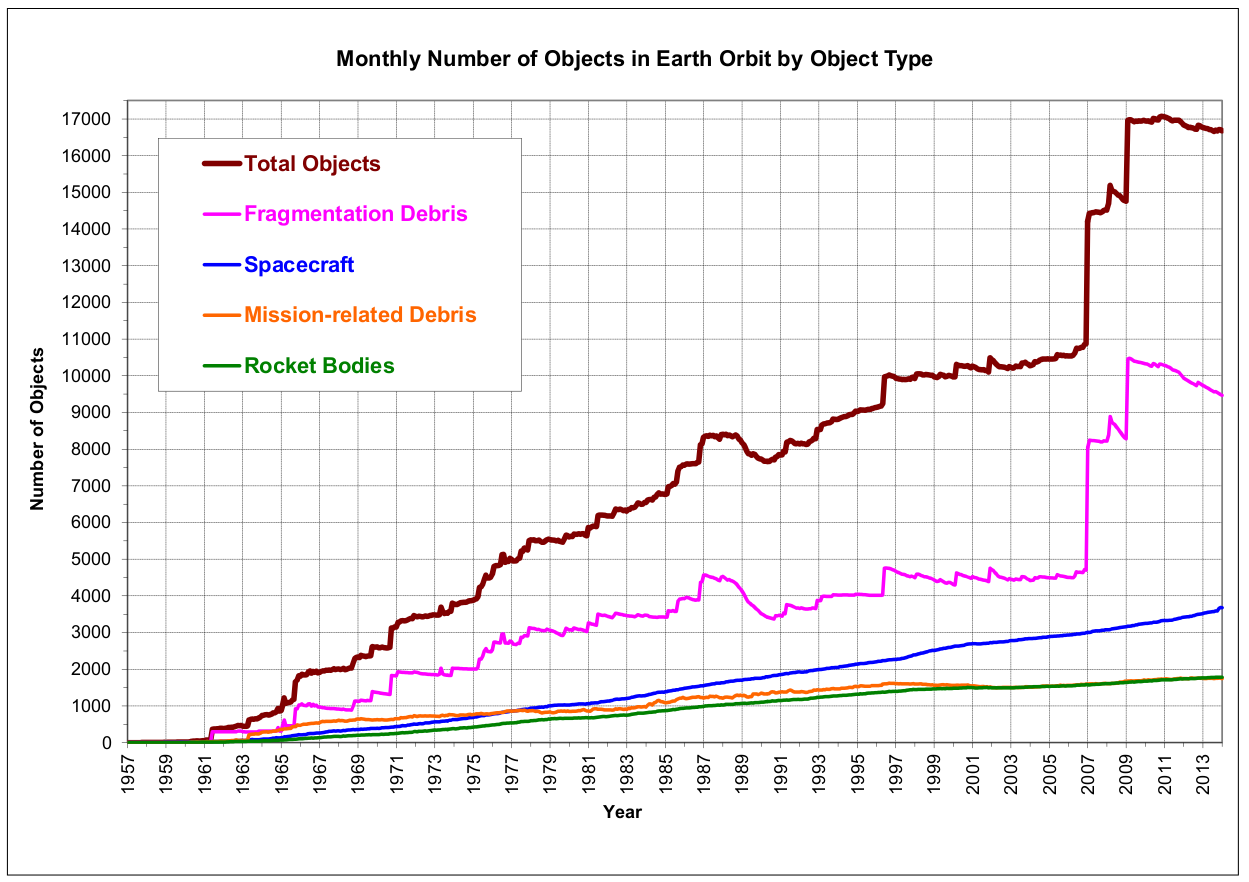
\includegraphics[width=0.8\textwidth]{imagenes/numero2014}
  \caption[Cantidad de Objetos catalogados al 2014]{Cantidad de Objetos catalogados al 2014 - Se distingue el incremento abrupto producto de las fragmentaciones del Fengyun Chino en 2007 y de la colisi\'on entre el IRIDIUM y el Kosmos en 2009.Extra\'ido de \citep{ODQN14}}
  \label{fig:cantidad2014}
\end{figure}

En esta problem\'atica, se produce una retroalimentaci\'on negativa, en donde, a partir del incremento de objetos, en particular en las \'orbitas LEO, aumentan las colisiones, convirti\'endose las mismas, a su vez, en las principales fuentes de generaci\'on de desechos.\\ 

La Figura \ref{fig:causadesechos} muestra que el porcentaje del remanente de desechos producto de rupturas debido a diferentes causas, fue modific\'andose en los \'ultimos a\~nos. Las distintas pol\'iticas de mitigaci\'on en relaci\'on a explosiones intencionales, restos de combustibles, el tratamiento de las bater\'ias y la protecci\'on de los materiales frente a impactos, han reducido el n\'umero de desechos asociados a estas cuestiones y a causas desconocidas; no obstante, los desechos generados por colisiones han aumentado.\\

\begin{figure}[!h]
  \centering
  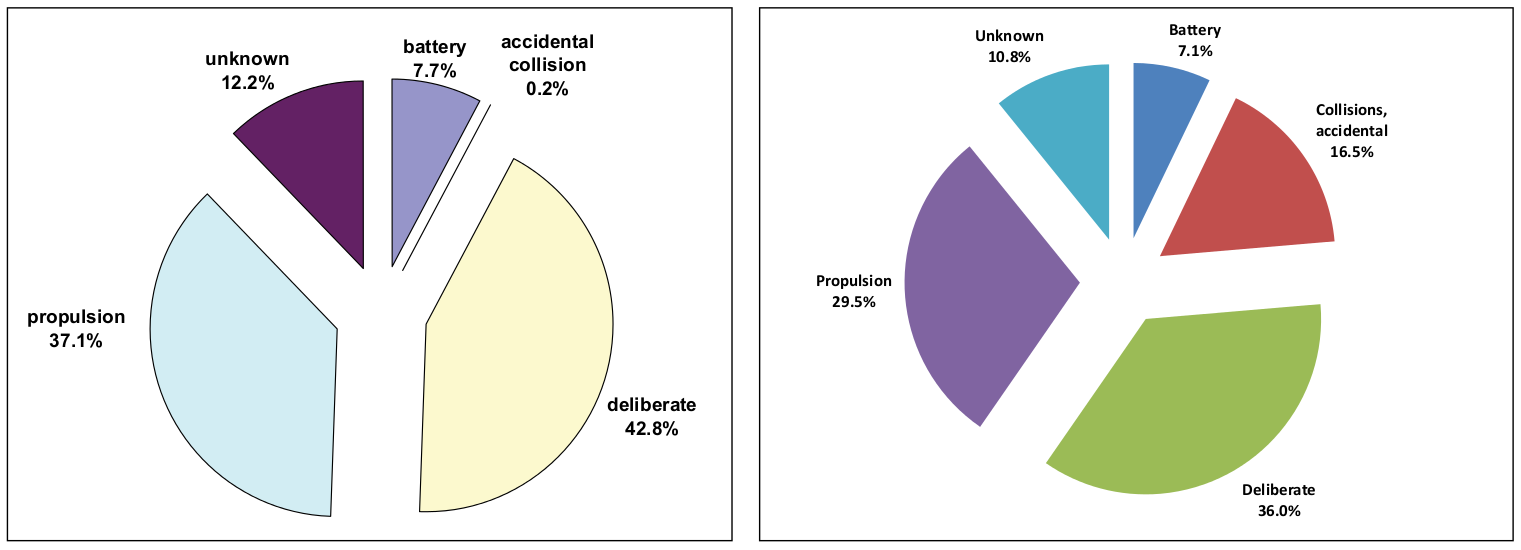
\includegraphics[width=0.8\textwidth]{imagenes/breakupsQNews}
  \caption[Evoluci\'on de las causas de la generaci\'on de Desechos]{Evoluci\'on de las causas de la generaci\'on de Desechos entre 2007 y 2016. Extra\'ido de \citep{ODQNum}}
  \label{fig:causadesechos}
\end{figure}

Conclusiones similares se desprenden del estudio de Karacalioglu \citep{karacalioglu2016impact}, cuyas simulaciones futuras se\~nalan que en los pr\'oximos a\~nos ser\'an las colisiones las que mayor n\'umero de desechos aporten al total de objetos que orbitan la Tierra en las \'orbitas bajas (Fig. \ref{fig:debriscollision}).\\

\begin{figure}[!h]
  \centering
  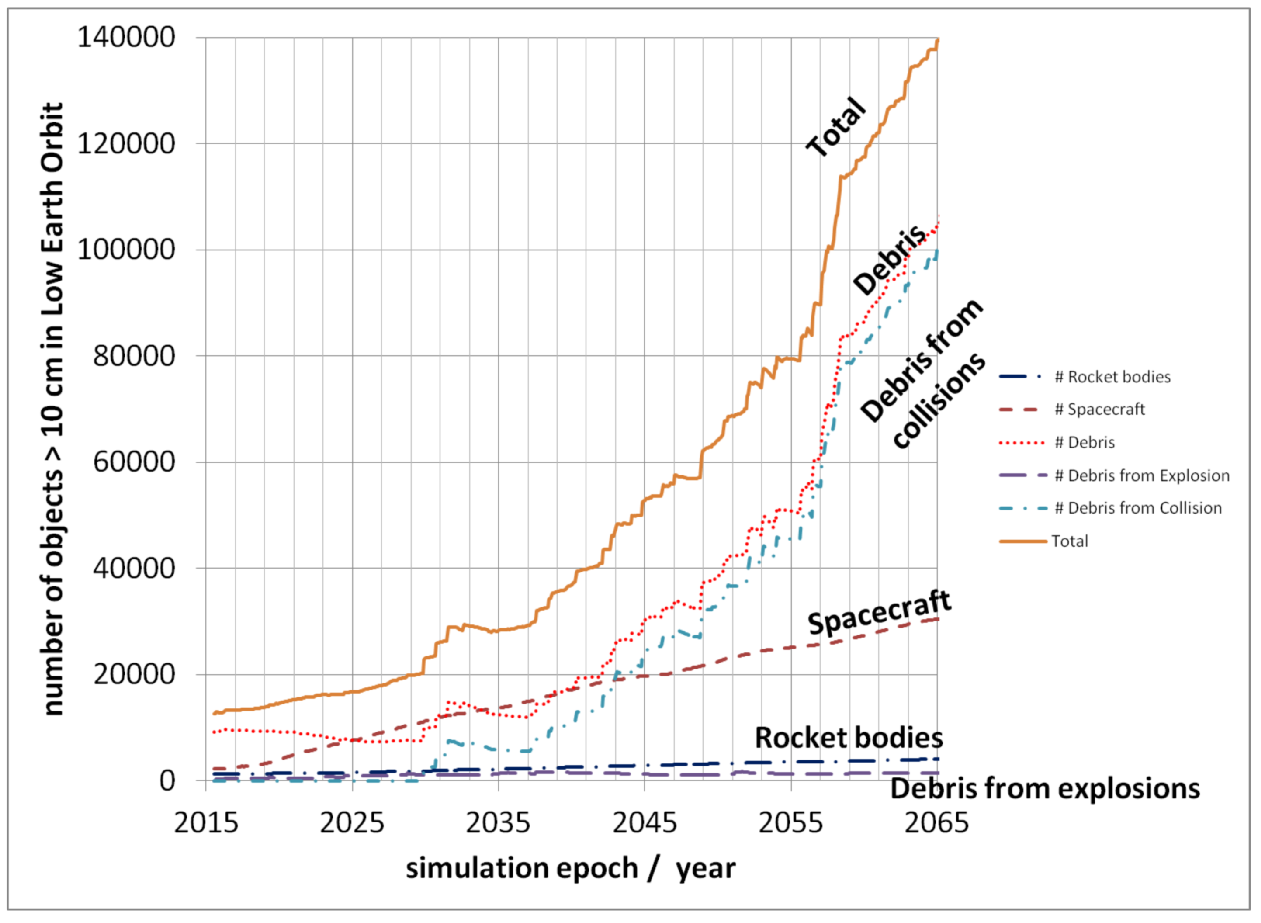
\includegraphics[width=0.7\textwidth]{imagenes/debriscollision}
  \caption[N\'umero de Desechos en las \'orbitas LEO desde 2015 al 2065]{N\'umero de desechos mayores a 10 cm, en las \'orbitas LEO desde 2015 al 2065. La mayor cantidad de desechos en el futuro ser\'an generados producto de las colisiones (curva celeste). Extra\'ido de \citep{karacalioglu2016impact}}
  \label{fig:debriscollision}
\end{figure}

Ya en 1978  estudios hechos por D. Kessler y Cour-Palais,
 \citep{kessler0}, anunciaban el riesgo del efecto en cascada que podr\'ian producir las colisiones, aumentando los desechos en un camino catastr\'ofico sin fin y mostrando que los desechos generados por colisiones superar\'ian los impactos por meteoritos.\\
 
 Por su parte los modelos de ingenier\'ia ofrecen una descripci\'on de los distintos efectos que producen los impactos, dependiendo del tama\~no del desecho. Ver Tabla \ref{tamanioDanio}\\
 
 \begin{table}[h]
 \caption[Da\~no seg\'un el tama\~no del desecho.]{Da\~no producido por el impacto con un desecho en funci\'on del tama\~no del desecho.}
\begin{tabular}[c]{c| l}
\hline
\hline
Tama\~no m\'inimo de la  &    Efecto\\
part\'icula que genera el efecto & \\
\hline
\hline
\multirow{ 7}{*}{100 $\mu$m }& * Da\~no significativo en sensores sensibles.\\
& (Las ventanas del transbordador requieren recambio)\\
& * Corta ataduras, anclajes y cables.\\
& * Penetraci\'on de las multicapas de aislaci\'on (MLI)\\
& * Penetraci\'on de las paredes con grosores de 300 a 500 $\mu$m.\\
& * Penetraci\'on de los tubos de calefacci\'on y radiadores.\\
& * Penetraci\'on de celdas solares.\\
\hline 
\multirow{ 5}{*}{1 mm }& * Cr\'ateres y perforaciones de 2 mm a 1 cm de di\'ametro\\
& dependiendo del tipo del material y el grosor.\\
& * Penetraci\'on de las paredes con grosores de 3-5 mm.\\
& Da\~no del equipamiento detr\'as de las paredes.\\
& *Penetraci\'on de tanques y cables externos.\\
\hline
\multirow{ 3}{*}{1 cm } & * Da\~no estructural y destrucci\'on de alguna parte impactada.\\
& * Penetraci\'on de todas las capas\\ %, incluyendo modulos tripulados\\
& con protecci\'on especial.\\
\hline
\multirow{ 2}{*}{10 cm } & * Destrucci\'on total del sat\'elite o del subsistema impactado.\\
& * Interferencia con observaciones astron\'omicas.\\
\hline
\multirow{ 2}{*}{1m}& * Partes s\'olidas de la plataforma pueden sobrevivir\\
& y reingresar a la atmósfera, incluso alcanzando la superficie.\\
\hline
\end{tabular}
\label{tamanioDanio}
\begin{flushleft}
\small {\it{Nota.}}  Extra\'ido de IADC 08/03, Versi\'on 2.1, Abril 2013
\end{flushleft}
\end{table}

\subsection{El estudio del riesgo de colisi\'on}\label{subsec:estudiocolision}

Para evitar impactos que comprometan significativamente la salud del sat\'elite, la nave debe contar con la capacidad de realizar una maniobra en los casos en los que el objeto de choque tenga un tama\~no considerable, a saber, mayor a los 10 cm de di\'ametro. No obstante, objetos de este tama\~no, pueden ser rastreados y catalogados, lo que permite predecir acercamientos y hacer an\'alisis de las distintas situaciones.\\

A partir del estudio de la situaci\'on orbital de los objetos y los errores involucrados, se estiman ciertos par\'ametros (Ver Sec. \ref{sec:probcol}) que luego son comparados a valores definidos bajo ciertos criterios para concluir si el sat\'elite se encuentra en una situaci\'on de riesgo.\\ 

Un an\'alisis completo del riesgo de colisi\'on abarca, (Fig. \ref{fig:estudiocolision}):

\begin{itemize}
\setlength{\itemsep}{0pt}
\item Identificar las situaciones de encuentro.
\item Analizar la situaci\'on del encuentro.
\item Ejecutar maniobras de mitigaci\'on del riesgo si fuera necesario.
\item Iterar el proceso en forma minuciosa para no ofrecer soluciones moment\'aneas que generen nuevos riesgos de colisi\'on.
\end{itemize}

\subsubsection*{Identificaci\'on de las situaciones de encuentro:}
A partir de los datos generados por las redes de rastreo (Sec.\ref{subsec:redes}), se propagan las trayectorias orbitales y, bajo ciertos criterios definidos previamente, se detectan los acercamientos no deseados.\\
En esta idea subyace la definici\'on de {\it{Encuentro}}.\\

Son pocos los organismos y agencias capaces de realizar este procedimiento, incorporando a sus predicciones todos los objetos catalogados y/o rastreados. En un esquema m\'as simplificado, el inter\'es se enfoca en una misi\'on en particular y se desarrollan filtros, para procesar encuentros analizando una menor cantidad de objetos.\\


\subsubsection*{An\'alisis de la situaci\'on del encuentro: }
El mismo consiste en estudiar el encuentro con mayor profundidad y detalle, sumando informaci\'on m\'as confiable en la determinaci\'on orbital, y calculando par\'ametros estad\'isticos, como la probabilidad de colisi\'on, \ac{PoC}.\\

A medida que se aproxima la fecha en la que se predice el encuentro, se tiene mejor conocimiento de la \'orbita de los objetos involucrados, pero menor tiempo de reacci\'on en la toma de decisiones. Es decir, en el an\'alisis del encuentro se busca un balance entre los tiempos que conlleve el estudio para alcanzar la confiabilidad necesaria, y el margen que se requiere para, por ejemplo, planificar una maniobra. En este \'item en particular se enfoca este trabajo.\\

\subsubsection*{Realizaci\'on de una maniobra:}
Si la situaci\'on lo ameritara, la \'unica manera de evitar una colisi\'on es la {\bf{realizaci\'on de una maniobra}}, conocidas como Maniobras de Mitigaci\'on de Riesgo o \ac{RMM}. No obstante, modificar la trayectoria de un objeto, siempre presupone una evaluaci\'on a priori de que no vaya a producirse una colisi\'on. De manera, que en este punto, se realizan propagaciones con las posiciones estimadas durante y luego de la maniobra, y se itera el proceso para estas nuevas posiciones contra el cat\'alogo de objetos.\\ 


% La exitosa Misi\'on SAC-D/AQUARIUS de la CONAE en convenio con la \ac{NASA}, contabiliz\'o del orden de cinco RMM registradas, a lo largo de su vida \'util [10]. Mientras que la \ac{ISS} realiza casi una maniobra de riesgo de colisi\'on por año, dada su envergadura.\\

\begin{figure}[!h]
  \centering
  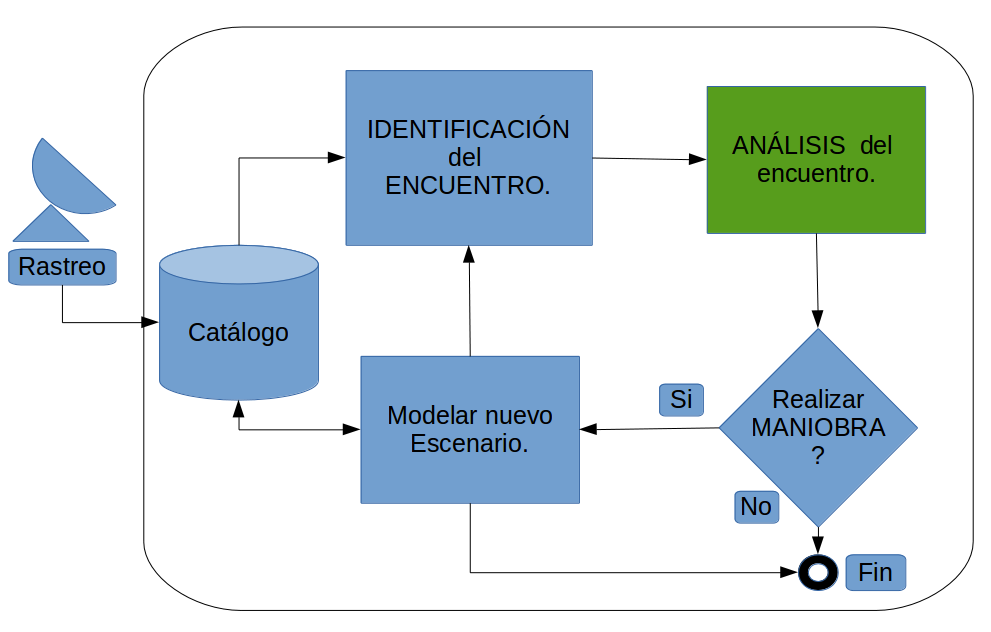
\includegraphics[width=0.6\textwidth]{imagenes/estudiocolision}
  \caption[Estudio de Colisi\'on]{Esquema de alto nivel de los procesos en un estudio completo de riesgos de colisi\'on. (Se indica en color verde, la etapa que se desarrolla en este trabajo.)}
  \label{fig:estudiocolision}
\end{figure}


% CONCEPTO DE MIDDLE MAN.\\
% CONCEPTO DE COLLABORATIVE WORK ENVIRONMENT. (close loop process)

\subsection{Rastreo y cat\'alogos}\label{subsec:redes}

En los catálogos actuales se registran objetos mayores a los 10 cent\'imetros en las regiones LEO monitoreadas con radares, y mayores a 1 metro en las \'orbitas \ac{GEO} observadas con telescopios \'opticos.\\
 
La entidad militar \ac{USSTRATCOM} de los Estados Unidos de Am\'erica (EE.UU) mantiene un catálogo con 18347 objetos conocidos (al 4 de Abril de 2017). Para su construcci\'on y mantenimiento, utiliza la Space Surveillance Network (SSN), que posee m\'as de 20 sensores civiles y militares a lo largo de todo el mundo (Fig.\ref{fig:usnet}).\\

\begin{figure}[!h]
  \centering
  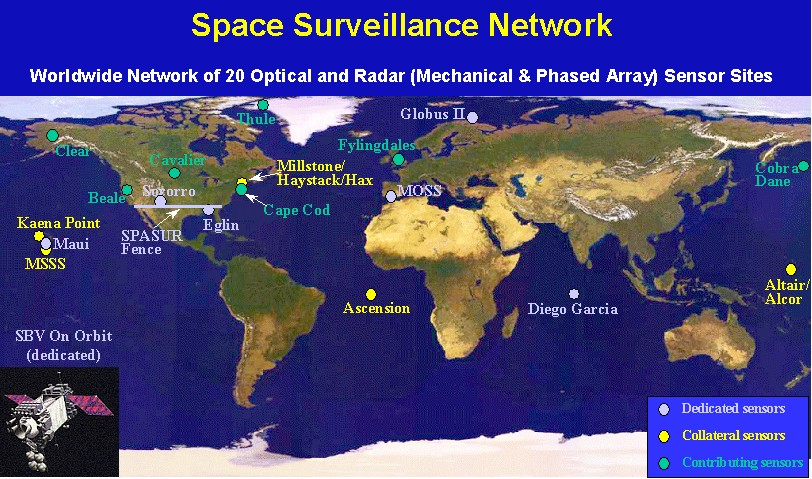
\includegraphics[width=0.7\textwidth]{imagenes/SpSNet}
  \caption[USSTRATCOM - SSN]{US. Strategic Command Space Surveillance Network. Extra\'ido de https://en.wikipedia.org/wiki/United\_States\_Space\_Surveillance\_Network}
  \label{fig:usnet}
\end{figure}

Rusia es la \'unica naci\'on, aparte de los EE.UU, que cuenta con un sistema de rastreo que le proporciona una base de datos de objetos espaciales artificiales significativa y actualizada. A su vez, independiente del gobierno Ruso, el Keldysh Institute of Applied Mathematics (KIAM) promueve la red internacional: International Scientific Optical Network (ISON), que ofrece uno de los programas coordinados de monitoreo de desechos m\'as importante.
La red cuenta con 30 telescopios en el rango de 0.5 a 2.6 metros de di\'ametro, repartidos en 20 observatorios de 8 pa\'ises en todo el mundo.\\

Por su parte, la ESA inici\'o programas de monitoreo hace ya varios a\~nos. En la actualidad predominan las investigaciones realizadas por las agencias espaciales: la Agenzia Spaziale Italiana (ASI) de Italia, el  British National Space Centre (BNSC) de  Inglaterra, el Centre National d'Études Spatiales (CNES) de Francia, y el Deutsche Zentrum fur Luft- und Raumfahrt  (DLR) de Alemania, con el apoyo de la industria, institutos de investigaci\'on y universidades. En los \'ultimos 10 a\~nos han estado trabajando en forma coordinada para implementar un Sistema Europeo de Vigilancia Espacial.
A tal fin cuentan con varios telescopios \'opticos como el Zeiss de 1 metro de Tenerife, el Schimdt y Tarot en Francia, o los sensores PIMS (Passive Imaging Sensors) del Reino Unido, y con importantes radares, como el TIRA (Tracking and Imaging Radar) en Alemania, o los m\'as modernos EISCAT Y EICAT 3D (European Incoherent Scatter Radar) que logran detecciones de objetos del orden de los cent\'imetros a distancias de 800 kil\'ometros.


% \begin{verbatim}
%  Settecerri, T. J et al – “Haystack measurements of the orbital debris environment” – Advances in Space Research 1999.
% Mehrholz, et al – “Beam-park experiments at FGAN” –  AdSpR 2004.
% Igor Molotov, et al – “Faint High Orbital Debris Observations with ISON Optical Network” – 
% Proceedings of the Advanced Moui Optical and Space
% \end{verbatim}



\section{Las regulaciones nacionales e internacionales}

Dado el car\'acter global de esta problem\'atica, distintas naciones y agencias internacionales con gran desarrollo y actividad espacial, se han estado organizado en la b\'usqueda de acuerdos y buenas pr\'acticas. Entre los organismos que coordinan las recomendaciones, se encuentran:\\

\begin{itemize}
\item COPUOS: Committee of the Peacefull Uses of Outer Space, \ac{ONU}
\item IADC: Inter-Agency Space Debris Coordination Committee
\item CCSDS: Consultative Committee for Space Data Systems
\end{itemize}

La NASA fue la primera en adoptar un conjunto de lineamientos para la mitigaci\'on de los desechos espaciales en 1995, que fueron posteriormente incorporados por el gobierno de EE.UU en 1997. \\

En el a\~no 2002 el IADC conformado por diez pa\'ises y la ESA, elabor\'o un nuevo conjunto de lineamientos.
Finalmente en 2007 el subcomit\'e cient\'ifico y tecnol\'ogico del COPUOS aun\'o los esfuerzos y reuni\'o todos los trabajos previos, logrando un consenso en los lineamientos definitivos promulgados por la ONU en 2008, \citep{nasaprogramme}.\\

En lo que respecta a los l\'imites de este trabajo, podemos citar las siguientes Normas, Recomendaciones y Legislaci\'on:\\

\begin{itemize} 
\item Convenio sobre Responsabilidad Internacional por da\~nos causados por objetos espaciales. ONU - (29-03-72)
\item Ley 23.335 (19-08-86) - Arg. Suscribe al Convenio de ONU.
\item Space Debris Mitigation Guidelines - \citep{iadcguide}
\item ISO 24113:2011 {\it{Space Debris mitigation requirements.}}
\item ISO/TR 16158:2013 {\it{Space Systems - Avoiding collision with orbiting objects.}}
\item ISO 19389:2014 {\it{Space data and information transfer Systems.}} Conjunction Data Message: specifies a standard message format for use in exchanging spacecraft conjunction information between originators of Conjunction Assessments (CAs) and satellite owner/operators and other authorized parties.
\item {\it{Guidelines for the long-term sustainability of outer space activities}}. Vienna, 8-17 de Junio de 2016.
\item {\it{CCSDS 508.0-B-1, Conjunction Data Message Recommended Standard}} - \citep{CDM}
\end{itemize}

\section{Antecedentes}\label{sec:antecedentes}
En este contexto, ya existen claros antecedentes que abordan la problem\'atica con sus respectivos soportes inform\'aticos. Ver Tabla \ref{tab:sisal}.
\begin{table}[!h]
\caption[Sistemas de Alerta]{Sistemas de Alertas de distintas Naciones y Agencias}
\begin{tabular}{lp{5cm}p{6cm}}
\hline
Herramienta & Descripci\'on & Proveedor/Agencia\\
\hline
{\bf{CARA}} & {\it{Conjunction Assessment Risk Analysis}} & NASA Robotic Conjunction Assessment Risk Analysis group, en convenio con la empresa a.i. solutions, Inc.\\
\hline
{\bf{SOCRATES}} & {\it{Satellite Orbital Conjuction Reports Assessing Threatening Encounters in Space}}, servicio web v\'ia Celestrack.com & CSSI (Center for Space Standards \& Innovation) de la agencia AGI: Analytical Graphics, Inc.\\
\hline
{\bf{CRASS}} & {\it{Collision Risk Assessment tool}} & Desarrollado por la
empresa GMV, que presta servicios al Centro Europeo de Operaciones
Espaciales (ESOC) - Darmstadt, Alemania, \citep{alarconRodriguez}\\
\hline
{\bf{CAESAR}} & {\it{Conjuction Analysis and Evaluation Service, Alerts and Recommendations}} & Agencia francesa CNES, que utiliza como soporte el Software JAC {\it{Java for Assessment of Conjunctions}}, \citep{laporte}\\
%\hline
%closeap - ant\'on & & ESA\\
\hline
{\bf{CRAMS}} & {\it{Collision Risk Assessment and Mitigation System}} & Canadian Space Agency (CSA), \citep{babiker}.\\
\hline
\end{tabular}
\label{tab:sisal}
\end{table}

\section{La Comisi\'on Nacional de Actividades Espaciales (CONAE)}
De acuerdo con el Plan Nacional Espacial: {\bf{ Argentina en el Espacio 2004-2015}}, las misiones de la CONAE, fundamentalmente pensadas para observaci\'on de la Tierra, ocupan \'orbitas bajas de dise\~no estrat\'egico, (Fig. \ref{fig:Dvsaltura}). Es decir, se ubican en regiones de mucha demanda y en consecuencia se encuentran expuestas a un alto riesgo de colisi\'on.\\

En nuestro pa\'is, compete a la CONAE; quien tiene la facultad de mantener las relaciones con los organismos internacionales, garantizar que se cumplan los distintos convenios y acuerdos a los que Argentina ha adherido, como por ejemplo el {\it{Convenio sobre la Responsabilidad Internacional por da\~nos causados por objetos espaciales}}, suscrito por la Rep\'ublica Argentina el 29 de marzo de 1972 (LEY N 23.335, sancionada: Julio 30 de 1986 - promulgada: Agosto 19 de 1986.1).\\

As\'i mismo, siendo Argentina miembro de la ONU, es la CONAE la representante ante el COPUOS en materia de buenas pr\'acticas para la mitigaci\'on de la generaci\'on de desechos espaciales.\\

Como se indica en la Sec. \ref{subsec:redes}, las \'unicas naciones que cuentan con una red de rastreo con capacidad de detectar, rastrear y catalogar objetos son los EE.UU y Rusia. De manera que la Argentina planifica y ejecuta sus maniobras de riesgo a partir de informaci\'on que le proveen servicios externos.\\

\section{Planteo del Problema}

El desfavorable panorama futuro en materia de colisiones en \'orbita, obliga a los centros de operaciones a incorporar procedimientos y soportes, para la gesti\'on, el an\'alisis y la prevenci\'on de las colisiones.\\

Dependiendo de las distintas capacidades con que cuentan las agencias, estos sistemas incluyen desde: redes o instrumentos espec\'ificos de rastreo propios, cat\'alogos completos de los objetos capaces de ser rastreados, sistemas de detecci\'on anticipada de acercamientos de riesgo, sistemas de an\'alisis de situaciones de riesgo alertadas por agentes externos o contrataci\'on de servicios externos que resuelven la totalidad del an\'alisis incluyendo la sugerencia de las maniobras pertinentes.\\

Argentina no cuenta actualmente con una red de rastreo para generar sus propios cat\'alogos y tampoco se desarroll\'o a\'un un sistema que permita
analizar los cat\'alogos ya existentes de acceso p\'ublico para el estudio de riesgo de colisi\'on de sus misiones.\\

Para cubrir este aspecto, la CONAE contrata un servicio externo de asesoramiento y control para la predicci\'on de los acercamientos de riesgo y la planificaci\'on de las operaciones necesarias. Ofrecer un servicio que lo reemplace, es impensado y escapa por mucho a los alcances de este trabajo. Sin embargo, pueden ir realiz\'andose desarrollos que permitan una mayor comprensi\'on,  caracterizaci\'on y registro de los eventos, y a partir de esa informaci\'on evaluar la posibilidad de impulsar proyectos que involucren el abordaje de esta problem\'atica, ya sea en busca de poder poder predecir los acercamientos utilizando cat\'alogos ya existentes, o mismo de instalar/adaptar instrumental para el rastreo de los objetos espaciales.\\


En este trabajo se presenta una herramienta que tiene la capacidad de:

\begin{itemize}
\item Incorporar alertas de riesgo de colisi\'on, ya sea a trav\'es de un mensaje estandarizado o ingresados manualmente por un operador.
\item Mostrar mediante una interfaz gr\'afica amigable esos valores que se ingresaron.
\item Hacer un registro ordenado de las distintas situaciones.
\item Calcular con sus propios m\'etodos, los par\'ametros de caracterizaci\'on del riesgo, a fin de evaluar la precisi\'on y las limitaciones del software.\\
\end{itemize}

La herramienta ARxCODE para el An\'alisis de Riesgo por Colisi\'on con Desechos, que presentamos en esta tesis, consiste en un prototipo de software para ser utilizado por operadores con amplios conocimientos de din\'amica orbital y operaciones.\\

Su capacidad para automatizar la recepci\'on de mensajes de alerta y desglozar el contenido, para presentarlo en forma m\'as amigable, pretende ofrecer una clara visualizaci\'on del evento y un mayor conocimiento al operador, para enriquecer el di\'alogo e intercambio de informaci\'on con los organismos y agencias que proveen servicio y asesoramiento en las situaciones de riesgo.\\

Por otro lado, conociendo los objetos involucrados en un acercamiento y el instante de acercamiento m\'aximo, ARxCODE cuenta con la facilidad de realizar un procesamiento propio de los par\'ametros de riesgo. Este desarrollo se piensa como un planteo preliminar, para ser probado, perfeccionado y ampliado a largo plazo, con la intenci\'on de lograr cierta autonom\'ia en la generaci\'on de los alertas.\\

En un esquema operativo, ARxCODE funcionar\'ia incorporado a los servicios de Din\'amica Orbital, cuyas interfaces con los organismos externos y el centro de operaciones se representa en la Figura \ref{fig:arcodeInterface}.\\ 


\begin{figure}[!h]
\centering
  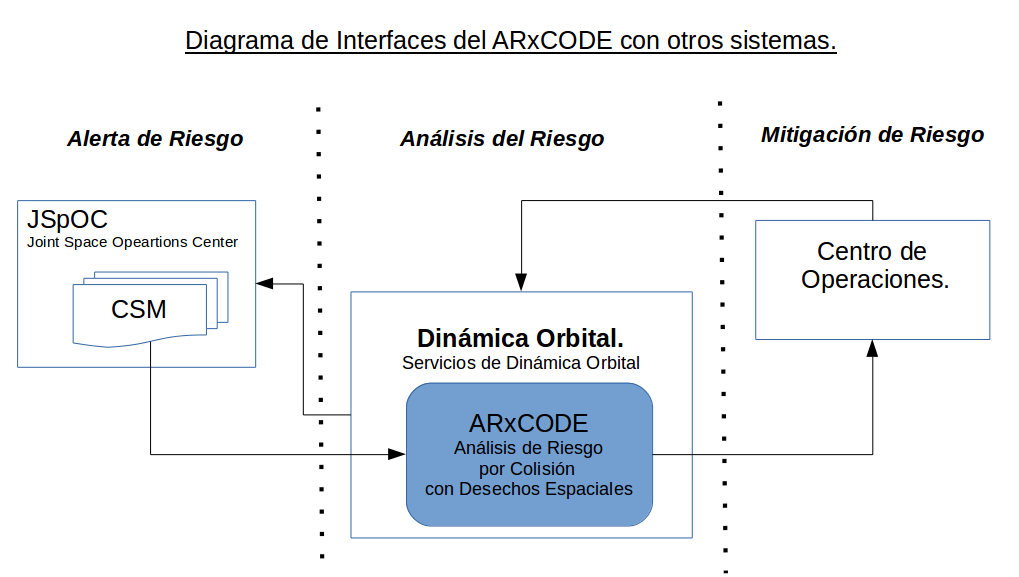
\includegraphics[width=0.7\textwidth]{imagenes/interfasessistemas}
  \caption[Interfaces del ARxCODE]{Esquema de Interfaces entre ARxCODE el orgamismo externo que envia el mensaje de alerta JSpOC, el Departamento de Din\'amica Orbital y el Centro de Control.}
  \label{fig:arcodeInterface}
\end{figure}



\section{Objetivos}

\subsection*{Objetivo principal}
Dise\~nar un procedimiento operativo frente a situaciones de alerta por riesgo de posible
colisi\'on con desechos espaciales y desarrollar un prototipo de software: ARxCODE, que
permita el c\'alculo de los par\'ametros de caracterizaci\'on del riesgo y facilite al analista la
la comprensi\'on y visualizaci\'on de la situaci\'on de riesgo en el di\'alogo con los servicios de alerta externos.\\

\subsection*{Objetivos espec\'ificos}
\begin{itemize}
\item Automatizar la recepci\'on y gesti\'on de los mensajes de alertas (CDM) por posibles
colisiones, que se reciben de organismos internacionales de rastreo.
\item Desarrollar una t\'ecnica que mejore la estimaci\'on de los errores en la posici\'on del desecho espacial.
\item Calcular la \ac{PoC} para caracterizar la situaci\'on de encuentro.
\item Desarrollar un prototipo de software (ARxCODE) para el procesamiento de la informaci\'on, el manejo de las notificaciones, la visualizaci\'on del evento y la generaci\'on de reportes.
\end{itemize}

\section{Estructura del trabajo}

A continuaci\'on de esta introducci\'on, en el cap\'itulo de {\bf{Marco Te\'orico}}; se describen los conceptos te\'oricos que se relacionan a la problem\'atica de las colisiones. Se detallan las distintas maneras en que se calculan las posiciones de los objetos seg\'un sean misiones operativas o desechos espaciales, los modelos de propagaci\'on, los formatos de publicaci\'on de la informaci\'on y los sistemas de referencia que utilizamos en este trabajo. En este cap\'itulo se dedica una secci\'on especial para el tratamiento de los errores en las posiciones y en las propagaciones, donde se describen el m\'etodo de Osweiler, \citep{osweiler} y el m\'etodo de propagaci\'on propuesto. Contin\'ua la secci\'on que contiene la informaci\'on te\'orica referida al c\'alculo de la probabilidad de colisi\'on y la descripci\'on de los tres m\'etodos implementados en este trabajo, a saber: m\'etodo del l\'imite \citep{alfano2008method}, m\'etodo de Lei-Chen, \citep{leichen} y m\'etodo de Akella \& Alfriend \citep{akellaAlfriend}.  Finalmente se presenta una secci\'on dedicada al mensaje estandarizado de alerta \ac{CDM}.

En el cap\'itulo 3: {\bf{ARxCODE: Especificaciones}}, se presentan las especificaciones del sistema. 

El cap\'itulo 4: {\bf{Metodolog\'ia de Desarrollo}}, se informa el plan de desarrollo y se detalla el entorno de trabajo. 

En el cap\'itulo 5 de {\bf{Aseguramiento de la Calidad}}, se describen las pruebas y actividades que fueron realizadas para asegurar la calidad del prototipo ARxCODE y se detalla el plan de V\&V y la gesti\'on de la configuraci\'on. 

En el cap\'itulo 6 de {\bf{Resultados}} se muestran los resultados m\'as significativos que se obtienen al utilizar el ARxCODE, y resultados intermedios que fueron necesarios para la generaci\'on de los productos finales. En cada caso se indica la fuente que se utiliz\'o para validarlos y se presentan valores comparativos en tablas o gr\'aficos. Al final del cap\'itulo se realiza un an\'alisis de los mismos. 

Finalmente el cap\'itulo 7, contiene las {\bf{Conclusiones}} y el trabajo a futuro. 


\endinput
\chapter{Marco Teórico}
\label{chap:marcoteorico}

\section{Introducci\'on}

Para el an\'alisis de posibles colisiones es necesario evaluar de forma anticipada las trayectorias de todos los objetos que orbitan la Tierra y detectar los acercamientos de riesgo. Si la predicci\'on de las posiciones fuera exacta, este estudio s\'olo implicar\'ia un esfuerzo computacional a resolver. No obstante, el movimiento orbital de los objetos no es ideal y las posiciones medidas o estimadas siempre acarrean una indeterminaci\'on; ya sea por: errores en la medici\'on, errores en el modelo de determinaci\'on orbital o errores en los modelos de predicci\'on orbital. A su vez, las indeterminaciones son mayores cuando se trata de desechos.\\

La t\'ecnica de detecci\'on de encuentros, consiste en realizar propagaciones de las posiciones de todo el cat\'alogo a partir de un instante inicial, en intervalos que por lo general, abarcan una semana hacia el futuro y medir las distancias entre los objetos. Se define un volumen seguro rodeando al sat\'elite de inter\'es, y si alg\'un objeto externo se introduce dentro del volumen de riesgo, es decir, se acerca a una distancia m\'inima por debajo del umbral determinado, se considera una situaci\'on de riesgo.\\ 
Esta metodolog\'ia no tiene en cuenta los errores en la determinaci\'on de la posici\'on de los objetos, y por lo general deriva en falsas alarmas, con las que se corre el riesgo de realizar maniobras innecesarias o que pueden poner en mayor peligro a la misi\'on.\\
Una vez identificado un encuentro, para un estudio m\'as exhaustivo de la situaci\'on, adem\'as de la m\'inima distancia de acercamiento o {\it{miss distance}}, se calcula la PoC.  Esta \'ultima ofrece un panorama m\'as completo ya que incorpora los errores en las posiciones a trav\'es de las matrices de covarianza.\\

Como ya mencionamos (Sec. \ref{subsec:estudiocolision}), en este trabajo nos enfocamos en analizar las situaciones de encuentro ya identificadas y en particular, aquellas que involucran a misiones operativas y desechos espaciales.\\

En este cap\'itulo, en primer lugar, se presentan las distintas maneras en que se determinan las posiciones de los objetos, dependiendo de si son misiones operativas o desechos.\\
La posici\'on de la misi\'on operativa y los errores asociados a la misma, la provee el departamento de din\'amica orbital (Sec. \ref{sec:posMision}).
La posici\'on de los desechos, s\'olo es posible conocerla, utilizamos los datos p\'ublicos que ofrece el comando de defensa norteamericano, \ac{NORAD} a trav\'es de su p\'agina Space-Track {\footnote{http://www.space-track.org}}. Las posiciones son publicadas en formato \ac{TLE} (Sec. \ref{subsec:tleformat}), sin errores asociados, y son propagadas hasta el momento del encuentro con el modelo SGP4  \citep{hoots1980models}, que tampoco ofrece informaci\'on sobre los errores de propagaci\'on. Se dedica un \'item para presentar el modelo de propagaci\'on SGP4 (Sec. \ref{subsec:sgp4model}) y se agrega en este espacio una breve descripci\'on de los sistemas de referencia con los que se trabaj\'o.\\

La siguiente secci\'on describe el tratamiento de errores. Para el estudio de la estimaci\'on de los errores en la posici\'on inicial, se detalla el m\'etodo de Osweiler \citep{osweiler} que permite la construcci\'on de las matrices de covarianza a partir de un conjunto de TLEs, cuando no se cuenta con datos m\'as precisos.\\
Una vez calculada la matriz de covarianza de errores, asociada a la posici\'on inicial, ser\'a necesario propagarla al instante predicho para el encuentro. Para ello se propone la implementaci\'on de una tabla con valores estad\'isticos inferidos del an\'alisis comparativo de efem\'erides precisas de la misi\'on operativa y las propagaciones de los TLE.\\
Contin\'ua la secci\'on que explica el algoritmo para el c\'alculo de la PoC y finalmente se describe en detalle, la forma en que se comunican los acercamientos de riesgo (Sec. \ref{sec:anuncio}), por ejemplo mediante \ac{CDM}.
% Incorporar los estados de alerta de Nasa. (texto de la aseguradora Britanica que me paso Juan ... bla de UNLAM.)


\section{La posici\'on de los objetos involucrados}{\label{sec:posMision}}
Al estudio de posiciones orbitales se lo puede dividir en tres etapas: medici\'on y/o rastreo, determinaci\'on orbital y propagaci\'on orbital.

\begin{itemize}
\itemsep0em
 \item {\bf{Medici\'on y/o rastreo:}} Abarca las mediciones desde Tierra, con radares, instrumentos \'opticos, l\'aser o doppler; y en el caspo de las misiones operativas, sistemas de navegaci\'on abordo, como por ejemplo GPS (Global Positioning System).\\
 \item {\bf{Determinaci\'on Orbital:}} Consiste en la utilizaci\'on de modelos de la \'orbita, que incorporan las mediciones y datos del entorno espacial (atm\'osfera, radiaci\'on solar, etc ) para ajustar los par\'ametros del modelo. Son procesamientos que se realizan a posteriori y que ofrecen distintos grados de precisión seg\'un las consideraciones que se tengan en cuenta.\
 \item {\bf{Propagaci\'on Orbital:}} Es el proceso mediante el cual, se extrapolan hacia el futuro las \'orbitas calculadas mediante determinaci\'on orbital.\\
\end{itemize}


En nuestro planteo de riesgos de colisi\'on entre misiones operativas y desechos espaciales, existen dos abordajes distintos respecto de las posiciones, ya que cada uno de los objetos involucrados utiliza metodolog\'ias y modelos diferentes.

\subsection{La posici\'on de la misi\'on operativa}

Con una misi\'on operativa se mantiene el contacto y se la puede comandar. Los sistemas de navegaci\'on abordo permiten un registro permanente de las posiciones y velocidades del sat\'elite. Esos registros se utilizan en los ajustes de los modelos de determinaci\'on orbital, que se realizan en procesamientos posteriores y se generan efem\'erides orbitales de mucha precisi\'on, cuyos errores resultan del propio procesamiento.\\
Para este trabajo se tuvo acceso a los productos orbitales de una misi\'on operativa, cuyas efem\'erides se plasman en archivos de texto plano, tabuladas cada un segundo, en el sistema de referencia verdadero de la fecha TOD. Seg\'un se nos inform\'o, los mismos presentan errores del orden de  20 metros. (\textcolor{red}{comunicacion por mail}).\\
Estas {efem\'erides precisas y sus errores asociados, son las que deben utilizarse en los estudios de riesgo, no obstante, para las procesamientos de este trabajo, si bien fue posible contar con las efem\'erides precisas, no se tuvo acceso a datos de acercamientos de riesgos por motivos de confidencialidad. Raz\'on por la cual, las posiciones de todos los objetos se calcularon a partir de los TLE p\'ublicos y las efem\'erides precisa fueron utilizadas para el estudio de los errores de los TLE, en particular para la generaci\'on de la tabla con los valores estad\'isticos de las varianzas, que se utilizan para la propagaci\'on de errores al instante TCA, Sec. \ref{subsec:tablaprop}. \\

\subsection{La posici\'on del desecho espacial}
El desecho espacial no tiene capacidades operativas, de manera que la \'unica forma de determinar su posici\'on es mediante las redes de rastreo descritas en la introducci\'on.\\
Como en Argentina no contamos con capacidad de rastreo, ARxCODE fue dise\~nado para obtener los datos de los desechos en el formato TLE, que publica NORAD, mediante el sitio web Space-Track.\\
Si bien son los datos m\'as completos y difundidos, utilizar estos datos acarrea errores muy importantes, y sobre todo desconocidos. Es por eso que debe implementarse alg\'un m\'etodo que permita estimarlos.\\

En las secciones siguientes se explicita el formato de los TLE y se describe el modelo SGP4 que permite la propagaci\'on de los mismos.\\

\subsection{Los TLE}{\label{subsec:tleformat}}

El formato TLE es un modo hist\'orico de registro de datos orbitales de los objetos rastreados que orbitan la Tierra. Sus siglas  hacen referencia a las Dos L\'ineas (Two-Line) en las que se plasman los elementos orbitales medios, junto con datos adicionales, de un dado objeto, para un instante particular.

Como se detalla a continuación, en la primera l\'inea se encuentran los identificadores del objeto y el n\'umero de lanzamiento del año, el instante en el que fueron calculados los elementos, y parámetros de ajuste, como las derivadas de movimiento medio y el t\'ermino de frenado atmosf\'erico, BSTAR, que resultan necesarios para la propagación de los TLE con el modelo dinámico SGP4 (Sec. \ref{subsec:sgp4model}).

En la segunda l\'inea se ubican los elementos orbitales cl\'asicos medios: inclinaci\'on, longitud del nodo, excentricidad, argumento del perigeo, anomal\'ia media y el movimiento medio, de donde se extrae el valor del semieje. En este punto es importante resaltar el hecho de que se trata de elementos medios, promediados bajo ciertos criterios y metodologías, no siempre especificadas, de manera que no son una exacta analog\'ia con los elementos orbitales de la posici\'on real para el instante indicado.


\begin{center}
\fbox{\parbox[b]{0.8\linewidth}{
Ejemplo de un TLE de la Estaci\'on Espacial Internacional (ISS) \\

\noindent
{\bf{1 25544U 98067A   08264.51782528 -.00002182  00000-0 -11606-4 0  2927\\
2 25544  51.6416 247.4627 0006703 130.5360 325.0288 15.72125391563537}}\\

{\bf{LINE 1 Primera línea del TLE}}\\
1   01–01   Número de línea    1\\
2   03–07   Número de satélite 25544\\
3   08–08   Clasificación      U\\
4   10–11   Identificador internacional (últimos dígitos del año de lanz.) 98\\
5   12–14   Identificador internacionl (número de lanzamiento del año)     067\\
6   15–17   Identificador internacional (piece of the launch)     A\\
7   19–20   Época del año (últimos dígitos del año)     08\\
8   21–32   Época (día del año y fracción de la porción de día)     264.51782528\\
9   34–43   Derivada primera del movimiento medio dividida por dos.   −.00002182\\
10  45–52   Derivada segunda del movimiento medio. 00000-0\\
11  54–61   BSTAR término de frenado atmosférico. -11606-4\\
12  63–63   El número 0. (originalemente traía el tipo de efemérides) 0\\
13  65–68   Número de set. I\\
14  69–69   Checksum (modulo 10)  7\\

{\bf{LINE 2 Segunda l\'inea del TLE}}\\
1   01–01   Número de línea    2\\
2   03–07   Númera de satélite 25544\\
3   09–16   Inclinación (grados)     51.6416\\
4   18–25   Ascención Recta del nodo ascendente. (grados)   247.4627\\
5   27–33   Excentricidad (parte decimal)  0006703\\
6   35–42   Argumento del Perigeo (grados) 130.5360\\
7   44–51   Anomalía Media (grados) 325.0288\\
8   53–63   Movimiento Medio (revoluciones por día) 15.72125391\\
9   64–68   Número de órbita (revoluciones)  56353\\
10  69–69   Checksum (modulo 10)  7\\
}}
\end{center}

\subsection{El propagador SGP4}\label{subsec:sgp4model}
De acuerdo a una rese\~na hist\'orica presentada por Hoots \citep{hootshistoria}, los or\'igenes del SGP4 se remontan al a\~no 1960 en EE.UU, cuando se desarroll\'o el modelo General Simplificado de Perturbaciones SGP  ({\it{Simplified General Pertubations}}). Basado en los modelos anal\'iticos de predicci\'on orbital de Brower \citep{brouwer1959solution} y Kozai \citep{kozai1962second}, para su implementaci\'on, fue adaptado y modificado para evitar singularidades en \'orbitas particulares y para reducir el tiempo de c\'omputo. As\'i mismo se incluy\'o el efecto del frenado atmosf\'erico.\\
En 1964 se convirti\'o en el modelo de predicci\'on orbital principal del sistema de detecci\'on y rastreo de los Estados Unidos.
Sin embargo, en 1969 la cantidad de objetos catalogados imped\'ian a las computadoras de la \'epoca procesar todos los t\'erminos del modelo, por lo que fue necesario desarrollar una nueva versi\'on m\'as simplificada, que result\'o en el SGP4 que se puso en operatividad en el a\~no 1970.\\

Esta \'ultima simplificaci\'on (Lane and Hoots, 1979) consisti\'o en :\\
\begin{itemize}
 \item Retener s\'olo los principales t\'erminos que modelan el efecto secular que produce el frenado atmosf\'erico.
 \item Restringir el modelo gravitacional de Brower s\'olo a los t\'erminos de per\'iodo largo o corto, que no contengan a la excentricidad como factor.
\end{itemize}

La primera versi\'on liberada del c\'odigo fuente del SGP4 se public\'o en el Spacetrack Report Number 3 \citep{spacetrackreport3}.\\
En 2004 Hoots et al. public\'o un documento completo con todas las ecuaciones (incluidas las correspondientes al modelo para espacio profundo); incorporando resonancias, las fuerzas que ejercen otros cuerpos, el drag atmosf\'erico y otras perturbaciones en las t\'ecnicas matem\'aticas.\\

El SGP4 es actualmente, el \'unico modelo para el mantenimiento del cat\'alogo de objetos a bajas alturas que orbitan la Tierra. 

\subsection{Sistemas de Referencia}\label{subsec:sistRef}

\subsubsection*{TEME}
 Es un sistema inercial con origen en el centro de la Tierra, que utiliza como plano fundamental el Ecuador Verdadero. El eje {\it{x}} se ubica en el plano del Ecuador Verdadero y apunta en la direcci\'on del Equinoccio Medio, el eje {\it{y}} tambi\'en se ubica sobre el plano ecuatorial a $90^{\circ}$ del eje {\it{x}}, y el eje {\it{z}} apunta en la direcci\'on del eje de rotaci\'on de la Tierra, perpendicular al plano ecuatorial. Sus siglas hacen referencia a un Ecuador Verdadero y un Equinoccio Medio o \ac{TEME}. Si bien no es un sistema convencional estandarizado, es el sistema que utiliza NORAD para la generaci\'on y propagaci\'on de los TLE, por lo que se encuentra ampliamente difundido.
 
\subsubsection*{TOD}
 Al igual que el TEME, es un sistema inercial definido con origen en el centro de la Tierra, con plano fundamental el Ecuador Verdadero. Su eje {\it{x}} tambi\'en yace sobre el plano ecuatorial pero se orienta en la direcci\'on del Equinoccio Verdadero (de la fecha).\\
 En el ap\'endice \ref{App1} se describe en forma detallada la transformaci\'on de coordenadas del sistema TEME al sistema TOD.
 
\subsubsection*{Sistemas centrados en el objeto}
Los sistemas RSW y NTW son dos sistemas con origen centrado en el objeto. Esta caracter\'istica ofrece ventajas cuando se hacen estudios de movimientos relativos, como en las misiones de sistemas distribuidos, o en los acoplamientos entre naves y tambi\'en clarifican la influencia de ciertos efectos perturbativos, como por ejemplo el del frenado atmosf\'erico, muy notorio en la componente a lo largo de la velocidad.\\

\begin{figure}[!h]
\centering
\fbox{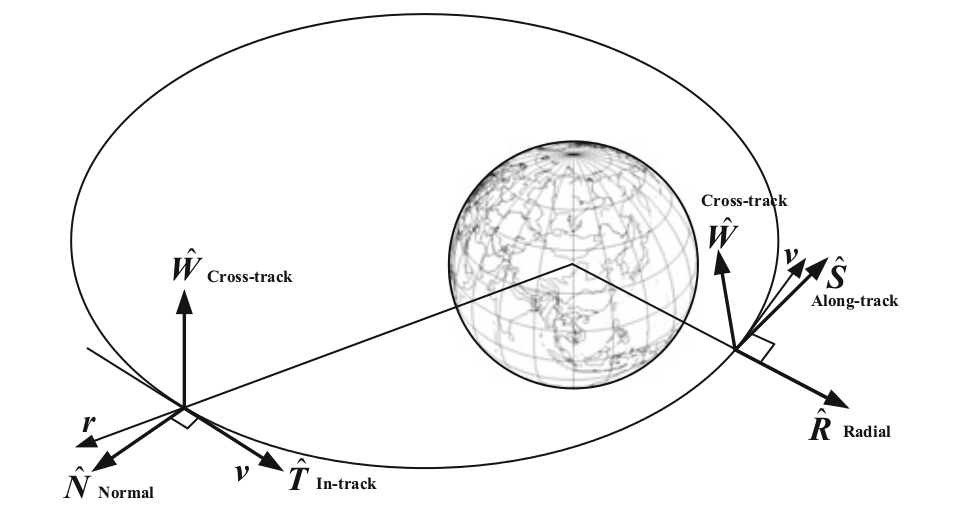
\includegraphics[width=0.8\textwidth]{imagenes/sistref}}
\caption[Sistemas de Referencia centrados en el Sat\'elite]{Sistemas de Referencia centrados en el Sat\'elite - extra\'ido de \cite{leichen}}
\label{fig:sistref}
\end{figure}


En el sistema {\bf{RSW}} la coordenada R (radial), tiene la direcci\'on del vector que une el centro de la Tierra con el objeto; la coordenada S ({\it{along-track or transverse}}), apunta en la direcci\'on perpendicular al vector R, a lo largo del movimiento pero no exactamente paralela a la direcci\'on de la velocidad (salvo en \'orbitas circulares o en \'orbitas el\'ipticas durante el apogeo y el perigeo); la coordenada W ({\it{cross-track}}), es perpendicular tanto a R como a S, es decir, normal al plano del movimiento. Este sistema tambi\'en se encuentra en la bibliograf\'ia como UVW, o \ac{RTN}.\\
Dado el vector posici\'on $\bar{r}$ y velocidad $\bar{v}$ del objeto de referencia, en un sistema inercial, en un momento dado; el sistema {\bf{RSW}} queda definido a partir de:\\


\begin{equation}
 \bar{R}=\frac{\bar{r}}{|\bar{r}|}, \quad \bar{W}=\frac{\bar{r}\times\bar{v}}{|\bar{r}\times\bar{v}|}, \quad \bar{S}=\bar{W}\times\bar{R}
\end{equation}

El sistema {\bf{NTW}} define el eje T (tangencial a la \'orbita) en la direcci\'on de la velocidad ({\it{in-track}}); el eje N (normal), en el plano orbital y perpendicular a la velocidad; y la componente W apunta en la direcci\'on perpendicular al plano orbital.\\
Dado el vector posici\'on $\bar{r}$ y velocidad $\bar{v}$ del objeto de referencia, en un sistema inercial, en un momento dado; el sistema {\bf{NTW}} queda definido a partir de:\\

\begin{equation}
 \bar{T}=\frac{\bar{v}}{|\bar{v}|}, \quad \bar{W}=\frac{\bar{r}\times\bar{v}}{|\bar{r}\times\bar{v}|}, \quad \bar{N}=\bar{T}\times\bar{W}
\end{equation}



Notar que ambos sistemas dependen de la posici\'on y la velocidad, es decir, que var\'ian con el tiempo.\\



%\subsubsection*{Sistema Geod\'esico Latitud y Longitud}


\section{El estudio de los errores}

La predicci\'on de un encuentro acumula los errores de las mediciones y de los modelos de la  determinaci\'on orbital, junto con los errores que introducen los modelos que extrapolan las posiciones hacia el futuro, en el proceso de propagaci\'on orbital.\\
Para el estudio de la situaci\'on de riesgo es necesario tener conocimiento, no s\'olo de las posiciones, sino tambi\'en de los errores asociados; raz\'on por la cual la estimaci\'on de errores es un proceso fundamental.\\ 
Esta caracter\'istica del problema, es la que conduce a estudiar probabilidades en los riesgos de colisi\'on.\\

En este trabajo se organiz\'o el tratamiento de errores en dos grandes secciones, en primer lugar, hay que tener en cuenta que en nuestro planteo siempre estar\'a implicado un desecho, por lo que ser\'a necesario conocer los errores que resultan de los TLE, ya que los mismos no son publicados. A tal fin, implementamos el m\'etodo de construcci\'on de matrices de covarianzas que propone \cite{osweiler}. Este m\'etodo permite construir una matriz de covarianza para la posici\'on de un TLE, utilizando el set de TLE de los \'ultimos 15 d\'ias anteriores al TLE en cuesti\'on. Este m\'etodo permite conocer los errores asociados a la posici\'on inicial.\\

En segundo lugar, para el an\'alisis de la situaci\'on del encuentro, ser\'a necesario contar con una t\'ecnica que ofrezca los errores que introducen la propagaci\'on del TLE hacia el futuro, es decir, hacia el momento predicho para le m\'aximo acercamiento. En este punto radica el aporte de este trabajo, ya que proponemos una forma para calcular la propagaci\'on de errores, a partir de estudios estad\'isticos del comportamiento de errores de los TLE (Sec. \ref{subsec:tablaprop}).\\

Debe tenerse en cuenta, que al utilizar TLE y el modelo SGP4  los datos propagados resultan en el sistema de referencia \ac{TEME}. Para poder comparar esos datos con las efem\'erides precisas publicadas en el sistema TOD, fue necesario hacer la respectiva transformaci\'on \ref{App1}.\\

\subsection{M\'etodo de Osweiler}\label{subsec:osw}
Es un m\'etodo que propone una manera de estimar los errores que se cometen al utilizar TLE para determinar la posici\'on y la velocidad de un objeto que orbita la Tierra.
El mismo consiste en utilizar un set de TLE de un intervalo de dos semanas, y considerar el \'ultimo TLE del set, al que denomina {\it{Primario}} como el valor real o verdadero.\\
A partir de esa premisa, propaga los TLEs anteriores hasta la \'epoca del TLE Primario y con las diferencias que resultan de la comparaci\'on, realiza los c\'alculos estad\'isticos de los valores medios y las varianzas, para construir la matriz covarianza correspondiente a la posici\'on del TLE Primario.\\

\subsubsection*{Esquema reducido del m\'etodo}

Dados:
\begin{itemize}
\itemsep0em
 \item N la cantidad de TLEs del set.
 \item $\bar{X}_{epoca} = $  Estimaci\'on del valor verdadero para la \'epoca.
 \item $\delta X_{epoca} = $ Residuos que se generan de la comparaci\'on del valor verdadero con los valores propagados.
 \item $m = $ Valores medios de los residuos.
 \item $P = $ Matriz de covarianza.
\end{itemize}

Se obtiene la matriz de covarianza $P$ a partir de:\\

\begin{equation}
 m=\sum_{i=1}^{N-1} \frac{(\delta X_{epoca})_{i}}{N-1} 
\end{equation}

\begin{equation}
 P_{epoca}=\sum_{i=1}^{N-1} \frac{(\delta X_{epoca}-m)_{i}(\delta X_{epoca}-m)_{i}^{T}}{N-1}
\end{equation}

\begin{figure}[!h]
\centering
\fbox{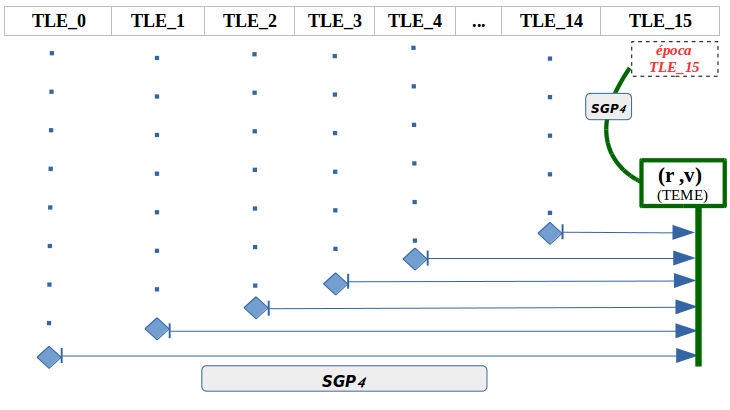
\includegraphics[width=0.8\textwidth]{imagenes/tleosw}}
\caption[M\'etodo de Osweiler para la generaci\'on de la matriz de covarianza]{Esquema del m\'etodo de Osweiler para la generaci\'on de la matriz de covarianza a partir de un set de TLEs}
\label{fig:tleosw}
\end{figure}

Este mismo m\'etodo se aplica a la misi\'on operativa, en aquellos escenarios en los que no se tiene acceso al dato de las efem\'erides precisas, como ocurre con los casos de estudio de validaci\'on que involucran misiones operativas de otras agencias.\\

\subsection{Propagaci\'on de errores utilizando TLE y efem\'erides precisas}\label{subsec:tablaprop}
Una vez que ya se conoce la matriz de covarianza del desecho para la posici\'on inicial, ser\'a necesario propagar esos errores al momento de m\'aximo acercamiento.\\
Dado que se desconocen los errores que introduce el propagador SGP4, fue necesario pensar una metodolog\'ia que permita hacer una estimaci\'on independiente.\\
Se propone un m\'etodo que utiliza las diferencias que resultan de los valores que ofrecen las efem\'erides precisas, en comparaci\'on con los valores que resultan de las propagaciones de TLE mediante SGP4. Se eval\'o la tendencia en una ventana temporal de seis meses y se calcularon los valores medios de los errores, en funci\'on de la cantidad de d\'ias de propagaci\'on.

\subsubsection*{Metodolog\'ia del estudio de la propagaci\'on de errores}\label{subsec:errorProp}
Pasos que se realizan, (Fig. \ref{fig:metodotabla}):
\begin{itemize}
\itemsep0em
\item Se selecciona un intervalo de 6 meses.
\item Se extraen los productos orbitales de la misi\'on operativa tabulados cada un segundo.
\item Se solicitan los TLE de la misi\'on correspondientes al intervalo.
\item Se toma el TLE del primer d\'ia y se lo propaga cada un segundo, para los pr\'oximos 7 d\'ias.
\item Se comparan las efem\'erides precisas con los valores que resultan de los TLE propagados.
\item Se calculan las varianzas en las coordenadas R, T y N, para cada d\'ia.
\item Se toma el TLE del d\'ia siguiente y se repite el procedimiento.
\item Se realiza la estad\'istica  de las diferencias agrupadas seg\'un sean, menores a un d\'ia y hasta 6 d\'ias.
\item Se plasman los resultados en una tabla que luego ser\'a usada por ARxCODE.
\end{itemize}

\begin{figure}[!h]
\centering
\fbox{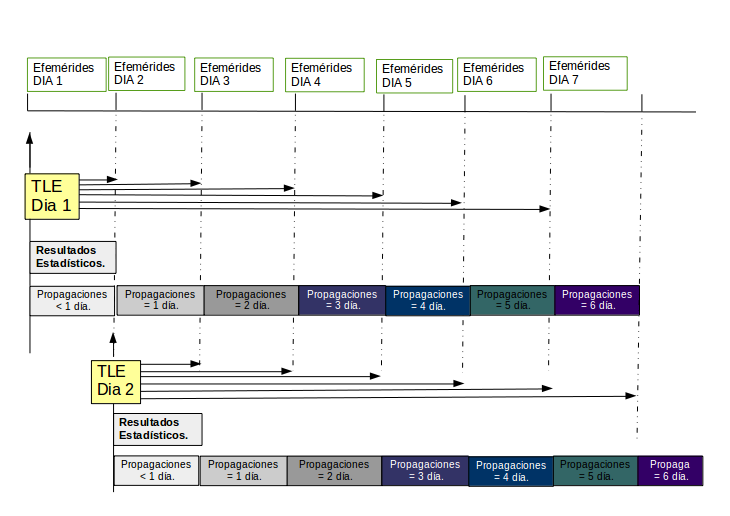
\includegraphics[width=\textwidth]{imagenes/metodoTabla}}
\caption[Descripci\'on del m\'etodo propuesto para la propagaci\'on de errores]{Esquema del m\'etodo propuesto para la estimaci\'on de la propagaci\'on de errores al utilizar TLE y el propagador SGP4. Los recuadros verdes contienen las efem\'erides precisas. Cada uno de los TLE se propagan para cada segundo, durante 7 d\'ias hacia adelante, y se comparan los valores de cada instante propagado con las efem\'erides precisas. Aqu\'i s\'olo se muestra la propagaci\'on de 2 d\'ias, pero el proceso se repite para los 6 meses del intervalo.}
\label{fig:metodotabla}
\end{figure}

A partir de las diferencias calculadas para cada segundo de cada d\'ia, se calculan valores medios y varianzas, por d\'ia.\\


\begin{figure}[!h]
\centering
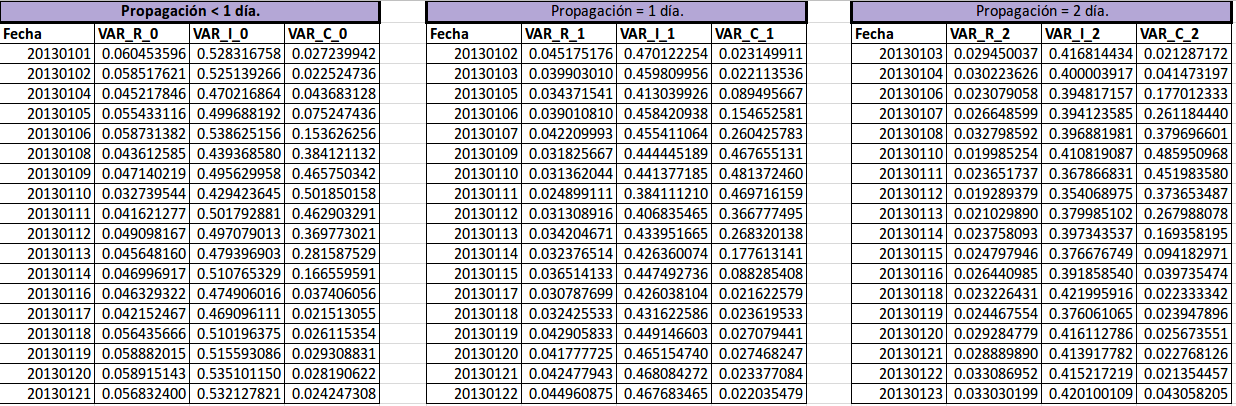
\includegraphics[width=\textwidth]{imagenes/tablacompleta}
\caption[Tabla de Estimaci\'on de errores.]{Fracci\'on de tabla con el total de datos calculados para la estimaci\'on estad\'istica. Se muestran s\'olo algunos d\'ias (primera columna de cada set) de los 6 meses, y los agrupamientos seg\'un sean respecto a propagaciones $< 1$ d\'ia, $= 1$ d\'ia o $= 2$ d\'ias}
\label{fig:tablacompleta}
\end{figure}

Luego se agrupan los valores seg\'un el intervalo de propagaci\'on, es decir, si son valores medios y varianzas de haber propagado 1, 2, 3 ... o hasta 6 d\'ias, y se toman los valores medios. Los resultados finales se plasman en una tabla cuyas columnas indican los valores medios de las varianzas por coordenada, y las filas los valores medios de las varianzas por intervalo propagado.\\

\begin{table}[!h]
\centering
\caption[Tabla con los valores medios para la propagaci\'on de errores.]{Resultados finales de los valores medios de las varianzas calculadas para la propagaci\'on de errores en funci\'on de los d\'ias de propagaci\'on}
\begin{tabular}{|l|c|c|c|}
\hline \hline
\rowcolor{yellow!35}
&$\sigma_R [km]$ &$\sigma_T [km]$ &$\sigma_N [km]$\\
\hline \hline
< 1 d\'ia & 0.05287535953&0.5110606907&0.09802202353\\
\hline
1 d\'ia & 0.03846388969&0.4517572281&0.09807457894\\
\hline
2 d\'ias & 0.02760890529&0.4086434248&0.09904162392\\
\hline
3 d\'ias & 0.01963580775&0.3765098311&0.09022336881\\
\hline
4 d\'ias & 0.01469071678&0.3577884914&0.1182060362\\
\hline
5 d\'ias & 0.01332578794&0.3557767231&0.1264764812\\
\hline
6 d\'ias & 0.01524829841&0.365815954&0.1607439516\\
\hline
\end{tabular}
\label{tab:resultatabla}
\end{table}

De la tabla \ref{tab:resultatabla} se extrae que la componente T, es la que mayor error introduce; con valores del orden de centenas de metros. Esto se debe a que el modelo de propagaci\'on SGP4 es d\'ebil en su representaci\'on del efecto que imprime el frenado atmosf\'erico en la componente asociada al movimiento o {\it{along-track}} T. 

\section{La Probabilidad de Colisi\'on}
Para el an\'alisis de una situaci\'on de riesgo, en general, se utilizan los par\'ametros:\\


\begin{itemize}
\centering
\itemsep0em
\item M\'inima distancia.
\item PoC.
\item M\'axima PoC.
\end{itemize}


Estos par\'ametros se calculan a partir de las \'orbitas predichas y las matrices de covarianza de los errores en el TCA.

Sean dos objetos; en nuestro caso una misi\'on operativa, {\it{sat}}, y un desecho, {\it{deb}}; de los cuales conocemos su posici\'on $\bar{X}_{sat0}=(\bar{x}_{sat},\bar{v}_{sat})$ y $\bar{X}_{deb0}=(\bar{x}_{deb}$,  $\bar{v}_{deb})$ y las matrices de covarianza de los errores, $C_{sat0}$, $C_{deb0}$, en un tiempo inicial,  $t_{sat0}$, y $t_{deb0}$ respectivamente. Todo referenciado al mismo sistema inercial de referencia, ya sea un sistema geoc\'entrico o \ac{ECI}; o el sistema del sat\'elite, \ac{RTN}.\\

En un planteo general, el estudio de una posible colisi\'on consiste en propagar hacia el futuro, mediante modelos (anal\'iticos y/o num\'ericos) las posiciones iniciales y las matrices de covarianza de errores; definir radios seguros (o de colisi\'on) para los objetos, y calcular la probabilidad de que la m\'inimia distancia entre ellos, sea menor a la suma de esos radios.\\
Un an\'alisis apropiado de situaciones de encuentro facilita la determinaci\'on del tiempo de m\'aximo acercamiento y las posiciones y matrices de covarianza para ese instante:  $\bar{X}_{sat}(TCA)$, $\bar{X}_{deb}(TCA)$, $C_{sat}(TCA)$, $C_{deb}(TCA)$.\\

Para su estudio, los encuentros pueden clasificarse seg\'un sean, encuentros cortos o largos. En particular en este trabajo, analizamos las situaciones de encuentros cortos.\\

\begin{itemize}
 \item {\bf{Encuentros cortos}}: se asume que el movimiento relativo presenta comportamiento lineal durante el breve lapsus del encuentro.
 \item {\bf{Encuentros largos}}: el encuentro no es lo suficientemente corto como para considerar movimiento relativo lineal.
\end{itemize}


En los encuentros cortos puede asumirse que:\\

\begin{itemize}
\itemsep0em
 \item El movimiento relativo es lineal.
 \item Los errores en la posici\'on durante el encuentro son constantes e iguales al del error en TCA.
 \item No hay errores en la velocidad.
 \item Los errores en la posici\'on se representan con una distribuci\'on gaussiana de tres dimensiones.
\end{itemize}

La probabilidad de colisi\'on se calcula en cada caso, conociendo: las posiciones, las matrices de covarianza de ambos objetos en el instante TCA, ($\bar{X}_{sat}(TCA)$, $\bar{X}_{deb}(TCA)$, $C_{sat}(TCA)$, $C_{deb}(TCA)$) y los radios de colisi\'on respectivos, $R1$ y $R2$.

\subsection*{C\'alculo de la PoC en encuentros cortos}

Distintos autores han desarrollado varios m\'etodos para el c\'alculo de la PoC (Ver tabla \ref{tab:trabajosPoc}). Todos ellos comparten las siguientes consideraciones:\\
\begin{itemize}
\itemsep0em
\item El error en la posici\'on puede representarse por una funci\'on de distribuci\'on Gaussiana en tres dimensiones (3D).
\item Tanto el objeto primario, como el desecho se mueven con movimiento rectil\'ineo de velocidad constante durante el encuentro.
\item Los errores en las velocidades se desprecian.
\item Los errores en las posiciones del objeto primario y del desecho no est\'an correlacionados.
\item Los errores en las posiciones son constantes durante el encuentro, al igual que la matrices de covarianzas correspondientes al TCA.
\end{itemize}

\begin{table}
 \centering
  \resizebox{\linewidth}{!}{
 \begin{tabular}{|c|l|}
 \hline \hline
 Autor/es & Metodolog\'ia\\
 \hline \hline
    Akella y Alfriend & Calcula la integral de superficie, del problema simplificado a 2D.\\
    \hline
    \multirow{4}{*}{Foster} & Calcula la integral de superficie del problema simplificado a 2D, utilizando la suma\\
    &  acumulada de anillos el\'ipticos conc\'entricos. Transforma el sistema a un sistema   \\
    & de referencia polar, e integra cada $0.5^{\circ}$ y un radio de $r_{a}/12$.\\
    & Es el m\'etodo que utiliza NASA para la ISS.\\
    \hline
    \multirow{4}{*}{Chan} & Desarroll\'o una soluci\'on anal\'itica en base a una serie infinita de\\
    &  t\'erminos que converge para la mayor\'ia de los valores m\'as comunes del problema,  \\
    &  a saber: radios combinados $r_{a}$ entre $1-100 m$, distancias m\'inimas  \\
    & de $10m-100km$ y covarianzas en el rango de $1m-10km$. \\
    \hline
    \multirow{3}{*}{Patera} & Transforma la integral de superficie a una integral de l\'inea\\
    &  de una dimensi\'on. Este nuevo planteo permite adaptar la secci\'on \\
    & de superfice a la forma de los objetos.\\
    \hline
    \multirow{2}{*}{Alfano (Serie)} & Utiliza una serie que combina las funciones error y\\
    & t\'erminos exponenciales para aproximar la integral de 2D.\\
    \hline
    \multirow{3}{*}{Alfano (Prob. M\'axima)} & Expresi\'on simplificada que permite hacer una estimaci\'on grosera\\
    & cuando no se cuenta con datos precisos de posici\'on o de la matriz de covarianza. \\
    & Utiliza una relaci\'on entre los radios combinados y la m\'inima distancia.\\
    \hline
 \end{tabular} }
 \caption[Trabajos sobre el c\'alculo de la PoC]{Distintos autores y trabajos para el c\'alculo de la Probabilidad de Colisi\'on PoC}
 \label{tab:trabajosPoc}
\end{table}

En su mayor\'ia, los m\'etodos que se mencionan en la tabla \ref{tab:trabajosPoc}, son aceptados en el est\'andar del mensaje de alerta, para el c\'alculo de la probabilidad de colisi\'on, ver Fig. \ref{fig:pagsana}.

% Los resultados del c\'alculo son sensibles a:
% 
% \begin{itemize}
% \itemsep0em
%  \item La geometr\'ia del encuentro.
%  \item La matriz de covarianza.
%  \item El tamaño de los objetos.
% \end{itemize}
  

\subsection{C\'alculo Simplificado de Lei-Chen}\label{subsec:pocsimp}

En este trabajo se implement\'o la estimaci\'on de un c\'alculo simplificado para la PoC, que propone Lei-Chen junto a otros autores en el libro 
{\it{Orbital Data Applications for Space Objects. Conjunction Assessment and Situation Analysis}} \citep{leichen}.

Lei-Chen se basa en el desarrollo anal\'itco de Chan \citep{chan2003improved} y otros estudios anteriores del problema del c\'alculo de la probabilidad de colisi\'on en encuentros cortos, que reducen el problema en tres dimensiones a un plano de encuentro.\\
Con este planteo, se reduce el problema a calcular la integral de la funci\'on de densidad de probabilidad (PDF) en dos dimensiones, sobre el \'area de la secci\'on circular de colisi\'on que se proyecta en el plano de encuentro.\\

La secci\'on circular de colisi\'on que se proyecta en el plano de encuentro, con radio $r_{a}$, est\'a centrada en las coordenadas $\mu_{x}$, $\mu_{y}$ del plano. Las desviaciones est\'andar que resultan de la matriz combinada de covarianzas de ambos objetos, proyectadas, son $\sigma_{x}$ y $\sigma_{y}$ Fig. \ref{fig:planoenc}.\\

\begin{figure}[!h]
\centering
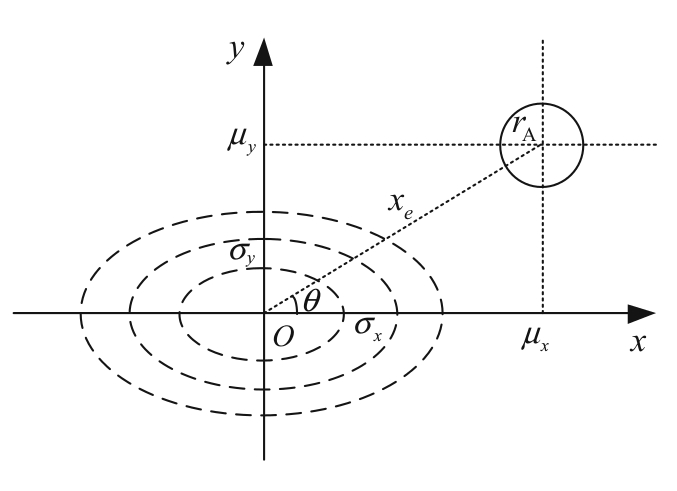
\includegraphics[width=0.6\textwidth]{imagenes/planodeencuentro}
\caption[Plano de Encuentro]{Esquematizaci\'on del plano de encuentro. Extra\'ido de \cite{leichen}}
\label{fig:planoenc}
\end{figure}

Finalemente, la expresi\'on del c\'alculo de la integral en dos dimensiones (2D), resulta:\\

\begin{equation}
 PoC=\int \int_{(x-\mu_{x})^{2}+(y-\mu_{y})^{2}\leq r_{a}^{2}} \frac{1}{2\pi\sigma_{x}\sigma_{y}} exp [-\frac{1}{2}(\frac{\mu_{x}^{2}}{\sigma_{x}^{2}}+\frac{\mu_{y}^{2}}{\sigma_{y}^{2}}) ] dy dx
 \label{eq:pocintegral}
\end{equation}

Tomando como referencia el trabajo de Chan \citep{chan2003improved} en la b\'usqueda de una expresi\'on anal\'itica que se construye mediante una serie convergente de infinitos t\'erminos; Lei-Chen presenta una expresi\'on para el primer t\'ermino de la serie y una f\'ormula recursiva de la serie, que resulta ventajosa para los m\'etodos de programaci\'on.\\

Como resultado de su trabajo \citep{lei2009rapid}, se encuentra que si se toma el primer t\'ermino de la serie como aproximaci\'on de la integral de la PoC,  el error de truncamiento es del orden de $10^{-5}$ o menor. Si se toman los dos primeros t\'erminos, el error de truncamiento es del orden de $10^{-9}$. Es decir, que para un primer an\'alisis, resulta suficiente considerar s\'olo el primer t\'ermino de la serie, cuya expresi\'on final es:\\


\begin{equation}
 PoC= \exp[-\frac{1}{2}(\frac{\mu_{x}^{2}}{\sigma_{x}^{2}}+\frac{\mu_{y}^{2}}{\sigma_{y}^{2}})][1-\exp(\frac{r_{a}^{2}}{2\sigma_{x}\sigma_{y}})]
 \label{eq:pocexpress}
\end{equation}

Ser\'a necesario incorporar m\'as t\'erminos en aquellos casos, en los que el radio de la secci\'on circular de colisi\'on y la m\'inima distancia sean mayores a las desviaciones est\'andar.

\subsubsection*{Expresi\'on de la PoC para \'orbitas circulares}

En la mayor\'ia de los casos, las \'orbitas son circulares o casi circulares. En esta configuraci\'on el m\'aximo acercamiento de los objetos ocurre siempre en posiciones cercanas a los puntos de m\'aximo acercamiento de las \'orbitas; y para las \'orbitas circulares esto se da exactamente en la l\'inea de de intersecci\'on de los planos orbitales de los dos objetos, ver Fig. \ref{fig:pocorbcirc} y \ref{fig:pocdistancia}.\\

\begin{figure}[!h]
\begin{minipage}[t]{0.48\textwidth}
 \centering
 \fbox{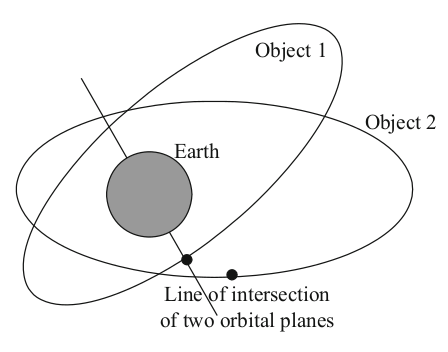
\includegraphics[width=0.8\textwidth]{imagenes/poccirc1}}
 \caption[M\'aximo acercamiento en \'orbitas circulares]{El punto de m\'aximo acercamiento en \'orbitas casi circulares ocurre siempre en puntos cercanos a los puntos m\'as pr\'oximos de las \'orbitas. Extra\'ido de \cite{leichen}}
 \label{fig:pocorbcirc}
\end{minipage}
\begin{minipage}[t]{0.48\textwidth}
 \centering
 \fbox{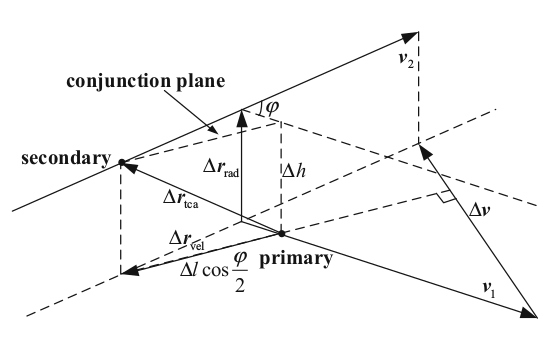
\includegraphics[width=\textwidth]{imagenes/poccirc2}}
 \caption[]{El m\'aximo acercamiento entre las \'orbitas $\Delta r_{rad}$ y el vector de m\'aximo acercamiento entre los objetos en el TCA, $\Delta r_{tca}$.}
 \label{fig:pocdistancia}
\end{minipage}
\end{figure}
 
Para el TCA, las coordenadas del centro del elipsoide de posici\'on del objeto secundario, son:\\
% 
\begin{gather}
 \mu_{x}=\Delta r_{rad}\\
 \mu_{y}=\Delta r_{vel}\\
\end{gather}
% 
Estas expresiones, proyectadas en el sistema RSW, ver Fig. \ref{fig:pocplano} y \ref{fig:pochorizontal}, resultan en:

\begin{gather}
 \mu_{x}=R\\
 \mu_{y}=\sqrt(S^{2}+W^{2})
\end{gather}

\begin{figure}[!h]
\begin{minipage}[t]{0.48\textwidth}
 \centering
 \fbox{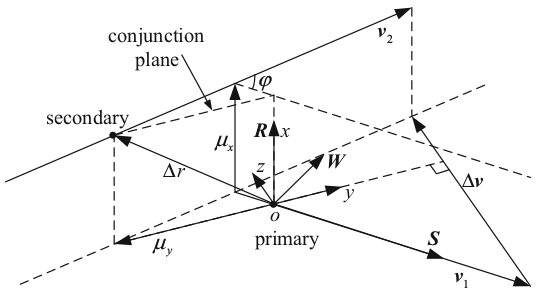
\includegraphics[width=0.8\textwidth]{imagenes/poccirc3}}
 \caption[Plano de encuentro y proyecci\'on del sistema RSW]{Definici\'on del plano de encuentro, {\it{conjuction plane}} y el sistema de coordenadas del objeto primario RSW. Extra\'ido de \cite{leichen}}
 \label{fig:pocplano}
\end{minipage}
\begin{minipage}[t]{0.48\textwidth}
 \centering
 \fbox{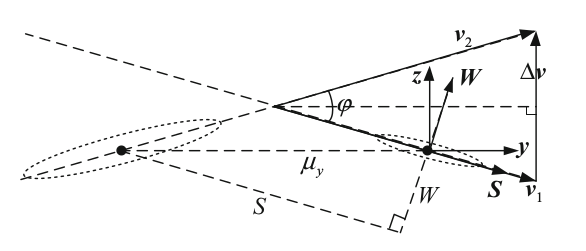
\includegraphics[width=\textwidth]{imagenes/poccirc4}}
 \caption[Proyecci\'on de los elipsoides de error al plano de encuentro]{Proyecci\'on de de los elipsoides de error al plano de encuentro. Extra\'ido de \cite{leichen}}
\label{fig:pochorizontal}
\end{minipage}
\end{figure}

\begin{gather*}
\sigma_{x}^{2}=\sigma_{R}^{2}=\sigma_{1R}^{2}+\sigma_{2R}^{2}\\
\sigma_{y}^{2}=\sigma_{SR}^{2}=\sigma_{S}^{2}cos^{2}(\frac{\phi}{2})+\sigma_{W}^{2}sin^{2}(\frac{\phi}{2})\\
\sigma_{S}^{2}=\sigma_{1S}^{2}+\sigma_{2S}^{2}\\
\sigma_{W}^{2}=\sigma_{1W}^{2}+\sigma_{2W}^{2}\\
\end{gather*}

% \subsection*{M\'etodo de Akella}
% En este trabajo para el c\'alculo de la PoC se utilizar\'a el m\'etodo de Alfriend \& Akella \citep{akellaAlfriend} ya que es conceptualmente simple y aunque tiene un alto costo computacional, es realizable por las m\'aquinas actuales en tiempos menores a un segundo.\\
% 
% El mismo requiere como entradas:
% \begin{itemize}
% \itemsep0em
% \item Conocer el instante de m\'aximo acercamiento: TCA (Time of Closest Approach).
% \item La posici\'on relativa del desecho respecto al objeto primario en el TCA.
% \item La velocidad relativa del desecho respecto al objeto primario en el TCA.
% \item Las matrices de error de ambos objetos.
% \end{itemize}
% 
% En los momentos pr\'oximos al encuentro, la posici\'on relativa de riesgo $\Delta r$ puede expresarse en funci\'on de un intervalo de tiempo respecto del TCA, es decir, $\Delta t_{tca}=t-t_{tca}$.
% 
% \begin{equation}
% \Delta r(t)=\Delta r_{tca}+\Delta v_{tca}(t-t_{tca})
% \end{equation}
% 
% Las matrices de covarianza de los errores que son calculadas para un momento dado t previo al TCA, deben ser propagadas. ({\bf{ver metodolog\'ia}})
% Dado que consideramos que los errores en las posiciones de ambos objetos no est\'an correlacionadas, ambas contribuciones pueden combinarse en una \'unica matriz, a partir de la suma de ambas.
% 
% \begin{equation}
% C=C_{p}+C_{d}
% \end{equation}
% 
% De $C$ s\'olo consideraremos la submatriz superior de la izquierda de dimensiones (3x3), que corresponde a los errores en las posiciones, con un $1 \sigma$.\\
% Dado que adem\'as asumimos que los errores en la posici\'on son de distribuci\'on normal en 3D, la funci\'on densidad de probabilidad $p(\Delta r)$ en momentos pr\'oximos al m\'aximo acercamiento queda definida por la expresi\'on {\bf{eq ..bla}}:
% 
% \begin{equation}
% p(\Delta r)=\frac{1}{\sqrt((2 \pi)^3det(C))} exp[-\frac{1}{2}\Delta r^TC^{-1}\Delta r]
% \end{equation}
% 
% Sean $R_{t}$ y $R_{r}$ los radios de las esferas que encierran a nuestra misi\'on principal y al desecho de riesgo, respectivamente. Se considera una situaci\'on de {\it{encuentro}} o {\it{riesgo de colisi\'on}}, al hecho de que estas esferas se intersecten, o lo que es lo mismo, si ocurre un acercamiento dentro de una esfera de {\it{radio de colisi\'on}} $R_{c}$, secci\'on $A_{c}$,  volumen $V_{c}$.
% 
% \begin{equation}
% R_{c}=R_{t}+R_{r} \qquad A_{c}=\pi R_{C}^{2} \qquad V_{c}=\frac{4}{3} \pi R_{c}^{3}
% \end{equation}
% 
% La probabilidad de colisi\'on $P_{c}$ se calcula a partir de la integral de volumen de la funci\'on densidad de probabilidad (eq) sobre la regi\'on esf\'erica $V_{c}$, centrada en el desecho de riesgo.
% \begin{equation}
% PoC=\frac{1}{\sqrt((2\pi)^3det(C))} \int \limits_{Vc} exp[-\frac{1}{2}\Delta r^TC^{-1}\Delta r]dV
% \label{eq:poc3d}
% \end{equation}
% 
% Puede demostrarse que esta integral de volumen puede reducirse a una integral de superficie mapeando el elipsoide  de los errores en la posici\'on, en contornos el\'ipticos de probabilidad constante sobre el B-plane {\bf{(citar a Foster)}}.
% 
% El B-plane es perpendicular al vector velocidad relativa $\Delta v_{tca}$ en el momento de m\'aximo acercamiento.
% A su vez, el vector $\Delta r_{tca}$ yace en el B-plane, como deja ver la ecuaci\'on de {\bf{zero-transit of the range-rate between the two objects}}:
% \begin{equation}
% \frac{\Delta v_{tca} \Delta r_{tca}}{\Delta r_{tca}}= \dot{\rho}_{tca}=0.0 \quad \rightarrow \quad t_{tca}
% \end{equation}
% 
% Definamos los vectores directores unitarios del plano como $X_{B}$ e $Y_{B}$, de acuerdo a las expresiones:
% 
% \begin{equation}
% X_{B}=\frac{\Delta r_{tca}}{|\Delta r_{tca}|} \quad Y_{B}=\frac{(\Delta r_{tca}) \times (\Delta v_{tca})}{|(\Delta r_{tca}) \times (\Delta v_{tca})|}
% \end{equation}
% 
% 
% A partir de estos vectores unitarios, se construye la matriz de transformaci\'on $R_{X_{B},Y_{B}}$ que mapea las matrices de covarianza en tres dimensiones $C=C_{x,y,z}$ a matrices de dos dimensiones en el B-plane $C_{B}$.
% 
% \begin{equation}
% C_{B} = C_{{X_{B},Y_{B}}} = R_{X_{B},Y_{B}} C R^{T}_{X_{B},Y_{B}}\\
% \end{equation}
% 
% \begin{equation}
% R_{X_{B},Y_{B}} =
% \begin{pmatrix}
% X_{B,X} & X_{B,Y} & X_{B,Z}\\
% Y_{B,X} & Y_{B,Y} & Y_{B,Z}
% \end{pmatrix}
% \end{equation}
% 
% Los ejes principales de los contornos el\'ipticos de probabilidad constante, quedan determinados a partir de los autovalores $\lambda_{i,B}(i=1,2)$ y los autovectores $\bar{e}_{i,B}$ que resuelven la ecuaci\'on:
% 
% \begin{equation}
% (C_{B} - \lambda_{i,B} I) \bar{e}_{i,B} = \bar{0}
% \end{equation}
% 
% Donde $I$ es la matriz identidad $2x2$.
% 
% Ahora, sea la elipse que representa los errores de posici\'on de $1\sigma$ en el B-plane:\\
% 
% \begin{itemize}
% \item El {\bf{semieje mayor}} queda definido por: $a_{1\sigma,B}=\sqrt(max(\lambda_{1,B},\lambda_{2,B}))$
% \item El {\bf{semieje menor}} queda definido por: $b_{1\sigma,B}=\sqrt(min(\lambda_{1,B},\lambda_{2,B}))$
% \item La {\bf{direcci\'on del semieje mayor}} ser\'a $\bar{e}_{a,B}$, con vector unitario: $ \bar{x}_{B}=\frac{\bar{e}_{a,B}}{|\bar{e}_{a,B}|}$
% \item La {\bf{orientaci\'on de $\bar{e}_{a,B}$}} respecto a la direcci\'on de la conjunci\'on $X_{B}$ la indica el \'angulo $\Phi_{B}$ (ver \ref{fig:bplane})
% \end{itemize}
% 
% \begin{equation}
% \Phi_{B}= arccos(\bar{x}_{B},X_{B})
% \end{equation}
% 
% \begin{figure}[!h]
% \centering
% 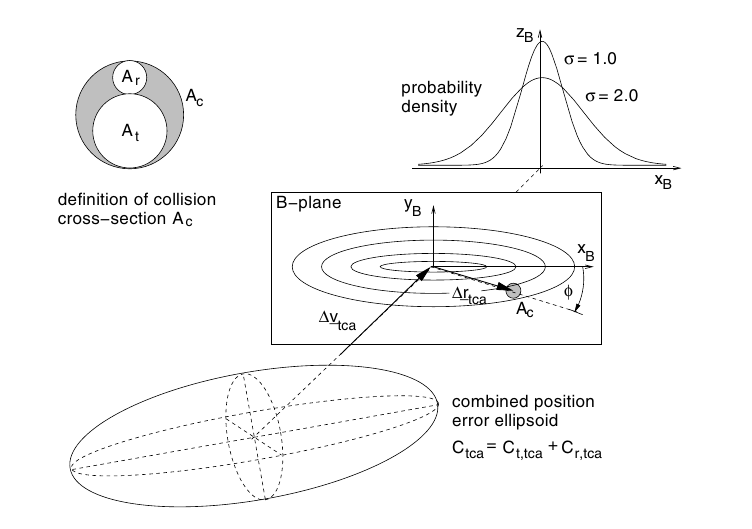
\includegraphics[width=0.5\textwidth]{imagenes/akellabplane}
% \caption{ B-plane (Adaptado de ....)}
% \label{fig:bplane}
% \end{figure}
% 
% Bien, consideremos ahora una posici\'on relativa de acercamiento $\Delta r_{B}$ ya proyectada en el B-plane. La integral de volumen de la probabilidad de colisi\'on de la Eq. \ref{eq:poc3d} se reduce a una integral de superficie sobre la secci\'on circular de colisi\'on $R_{c}$, proyectada en el B-plane y centrada a la distancia relativa predicha en el instante de m\'aximo acercamiento, $\Delta r_{tca}$
% 
% \begin{equation}
% P_{c} = \frac{1}{2 \pi \sqrt(det(C_{B}))} \int_{-R_{c}}^{+R_{c}} \int_{-\sqrt(R^{2}_{c}-x^{2}_{B})}^{+\sqrt(R^{2}_{c}-x^{2}_{B})} exp [- A_{B}] dy_{B} dx_{B}
% \end{equation}
% 
% \begin{equation}
% A_{B}=\frac{1}{2}\Delta r^{T}_{B} C^{-1}_{B} \Delta r_{B}
% \end{equation}



\section{Comunicaciones de riesgo de colisi\'on}{\label{sec:anuncio}}


A partir de las primeros accidentes, y da\'~nos por impactos, las agencias u organismos capaces de rastrear el ambiente espacial, comenzaron a implementar sistemas de comunicaci\'on para advertir sobre posibles colisiones. Las comunicaciones, que en sus or\'igenes eran mails particulares, fueron migrando a un mensaje formal y estandarizado y finalmente en Junio del 2013, el Consejo Consultivo para los Sistemas de Datos Espaciales, \ac{CCSDS}, public\'o el mensaje est\'andar recomendado que se utiliza en la actualidad, el: \ac{CDM} \citep{CDM}.\\
El {\it{CCSDS 508.0-B-1, Conjunction Data Message Recommended Standard}} describe en detalle la estructura del formato recomendado, aunque no propone formas de intercambio, dejando a las partes la potestad de acordar las distintas maneras de realizar la comunicaci\'on de los mismos, que, deber\'an ser detalladas en el documento de interfaces (ICD).\\

\subsection{El CDM}\label{subsec:cdm}

Es un mensaje estandarizado para el intercambio de informaci\'on entre los organismos capaces de detectar acercamientos y los due\~nos y/o operadores de los objetos involucrados en el encuentro.\\
Los CDM se env\'ian 72 horas antes del encuentro a los operadores a cargo y/o se disponibilizan en la p\'agina de space-track para usuarios con permisos especiales.\\
Los mismos se generan y se distribuyen de acuerdo a ciertos criterios.\\


\underline{Criterios de generaci\'on y env\'io de CDM}
\begin{itemize}
\item Para las {\bf{\'orbitas bajas}}, se consideran las situaciones en las que la m\'inima distancia total es menor a 1 kil\'ometro y la distancia relativa en la componente radial es menor a los 200 metros.\\

\item Para las regiones de los {\bf{sat\'elites geoestacionarios o las regiones medias}}, se env\'ian mensajes si la m\'inima distancia total es menor a los 10 kil\'ometros.\\
\end{itemize}


Su formato estandarizado unifica la informaci\'on que all\'i se publica y facilita la interoperatibilidad sin ambig\"{u}edades. Su estructura est\'a pensada para que sea de f\'acil interpretaci\'on tanto para personas como para m\'aquinas. Esto permite a los centros de control de las operaciones, la automatizaci\'on de los procesos de recepci\'on de los mensajes y ofrece la informaci\'on preprocesada, dejando m\'as tiempo para la toma de decisiones.\\

Son exclusivamente informativos, no imprimen recomendaciones ni sugerencias de acci\'on.
Y es importante destacar, que los centros de c\'omputo que los generan, no siempre cuentan con la informaci\'on de las pr\'oximas maniobras planificadas para los sat\'elites.\\

Es un mensaje codificado en formato ASCII, que puede distribuirse mediante un texto plano KVN, o por medio de un \ac{XML}. Contiene la m\'inima distancia, la PoC, el TCA y las posiciones y velocidades relativas en el momento de m\'inima distancia; entre muchos otros \citep{CDM}.\\

Ofrece la siguiente informaci\'on de un \'unico encuentro entre dos objetos: {\it{Object1}} y {\it{Object2}}:
\begin{itemize}
\item Las posiciones de  {\it{Object1}} y  {\it{Object2}} en el instante de m\'aximo acercamiento TCA. Los mismos en alguno de los sistemas de referencia m\'as utilizados, ver \ref{subsec:sistRef}.
\item Las covarianzas de las posiciones de los objetos en el instante TCA, tomando como referencia el centro de uno de ellos.
\item La posici\'on y velocidad relativa del {\it{Object2}} respecto al centro del {\it{Object1}}.
\item Informaci\'on relevante respecto a c\'omo fueron obtenidos los datos anteriores.
\end{itemize}


\subsubsection*{Estructura General del formato KVN}
El CDM en su formato KVN, consiste en un texto plano, con palabras claves o {\it{keywords}}, con su valor correspondiente.\\
El mensaje contiene una {\it{keyword}} por l\'inea, y el orden en que se presentan es fijo y est\'a determinado por el est\'andar, respetando la siguiente estructura:

\begin{itemize}
\itemsep0em
\item Un Encabezado.
\item Metadatos y datos relativos (datos que describen relaciones entre los objetos).
\item Metadatos. (datos respecto a c\'omo fueron creados los objetos).
\item Datos de cada uno de los objetos.
\item Comentarios opcionales.
\end{itemize}

Ejemplo con un peque\~no segmento:\\


\fbox{\parbox[b]{\linewidth}{
\begin{tabular}{llc}
CREATION\_DATE  &= 2010-03-12T22:31:12.000&\\
ORIGINATOR &= JSPOC& \\
MESSAGE\_FOR &= SATELLITE A&\\
MESSAGE\_ID &= 201113719185&\\
TCA &= 2010-03-13T22:37:52.618&\\
MISS\_DISTANCE &= 715 &[m] \\
RELATIVE\_SPEED &= 14762& [m/s] \\
RELATIVE\_POSITION\_R &= 27.4 & [m] \\
RELATIVE\_POSITION\_T &= -70.2 &[m] \\
RELATIVE\_POSITION\_N &= 711.8& [m]\\
...& ... & \\
COLLISION\_PROBABILITY &= 4.835E-05& \\
COLLISION\_PROBABILITY\_METHOD &= FOSTER-1992&\\ 
\end{tabular}
}}

\subsubsection*{Estructura General del formato XML}
El CDM en su formato \ac{XML} proporciona un m\'etodo est\'andar para acceder a la informaci\'on, facilitando el intercambio de datos electr\'onicos. Su estructura define el tipo de informaci\'on que hay en el documento, acelerando los procesos de b\'usqueda.\\
El XML del CDM, se agrupa como se muestra a continuaci\'on:

\begin{verbbox}
<header>
</header>
<body>
  <relativeMetadataData>
  </relativeMetadataData>
  <segment>
    <metadata>
    </metadata>
    <data>
    </data>
  </segment>
  <segment>
    <metadata>
    </metadata>
    <data>
    </data>
  </segment>
</body>\\
\end{verbbox}

\begin{center}
\fbox{\parbox[b]{0.5\linewidth}{
\theverbbox }}
\end{center}


\subsubsection*{Ejemplo de CDM}
A continuaci\'on se muestra un fragmento de ejemplo de un CDM en formato XML. Un ejemplo completo se adjunta en el (\textcolor{red}{Ap\'endice}).\\

\lstset{language=XML,basicstyle=\small}
\begin{lstlisting}
<?xml version="1.0" encoding="UTF-8"?>
<cdm xmlns:xsi="http://www.w3.org/2001/XMLSchema-instance"
xsi:noNamespaceSchemaLocation=
"http://sanaregistry.org/r/ndmxml/ndmxml-1.0-master.xsd"
id="CCSDS_CDM_VERS" version="1.0">
<header>
<COMMENT>Sample CDM - XML version</COMMENT>
<CREATION_DATE>2010-03-12T22:31:12.000</CREATION_DATE>
<ORIGINATOR>JSPOC</ORIGINATOR>
<MESSAGE_FOR>SATELLITE A</MESSAGE_FOR>
<MESSAGE_ID>20111371985</MESSAGE_ID>
</header>
<body>
<relativeMetadataData>
<COMMENT>Relative Metadata/Data</COMMENT>
<TCA>2010-03-13T22:37:52.618</TCA>
<MISS_DISTANCE units="m">715</MISS_DISTANCE>
<RELATIVE_SPEED units="m/s">14762</RELATIVE_SPEED>
<relativeStateVector>
<RELATIVE_POSITION_R units="m">27.4</RELATIVE_POSITION_R>
<RELATIVE_POSITION_T units="m">-70.2</RELATIVE_POSITION_T>
<RELATIVE_POSITION_N units="m">711.8</RELATIVE_POSITION_N>
<RELATIVE_VELOCITY_R units="m/s">-7.2</RELATIVE_VELOCITY_R>
<RELATIVE_VELOCITY_T units="m/s">-14692.0</RELATIVE_VELOCITY_T>
<RELATIVE_VELOCITY_N units="m/s">-1437.2</RELATIVE_VELOCITY_N>
</relativeStateVector>
<START_SCREEN_PERIOD>2010-03-12T18:29:32.212</START_SCREEN_PERIOD>
<STOP_SCREEN_PERIOD>2010-03-15T18:29:32.212</STOP_SCREEN_PERIOD>
<SCREEN_VOLUME_FRAME>RTN</SCREEN_VOLUME_FRAME>
<SCREEN_VOLUME_SHAPE>ELLIPSOID</SCREEN_VOLUME_SHAPE>
<SCREEN_VOLUME_X units="m">200</SCREEN_VOLUME_X>
<SCREEN_VOLUME_Y units="m">1000</SCREEN_VOLUME_Y>
<SCREEN_VOLUME_Z units="m">1000</SCREEN_VOLUME_Z>
<SCREEN_ENTRY_TIME>2010-03-13T20:25:43.222</SCREEN_ENTRY_TIME>
<SCREEN_EXIT_TIME>2010-03-13T23:44:29.324</SCREEN_EXIT_TIME>
<COLLISION_PROBABILITY>4.835E-05</COLLISION_PROBABILITY>
<COLLISION_PROBABILITY_METHOD>FOSTER-1992
</COLLISION_PROBABILITY_METHOD>
</relativeMetadataData>
\end{lstlisting}

A diferencia de los mensajes estandarizados anteriores, como el CSM:{\it{Conjunction Summery Message}}, el CDM ofrece un valor estimado para la PoC e indica el m\'etodo que se utiliz\'o para calcularlo. Estos m\'etodos (Ver Fig. \ref{fig:pagsana} ), son adem\'as los m\'etodos que el est\'andar sugiere para la implementaci\'on de los c\'alculos de PoC.\\

\begin{figure}[!h]
\centering
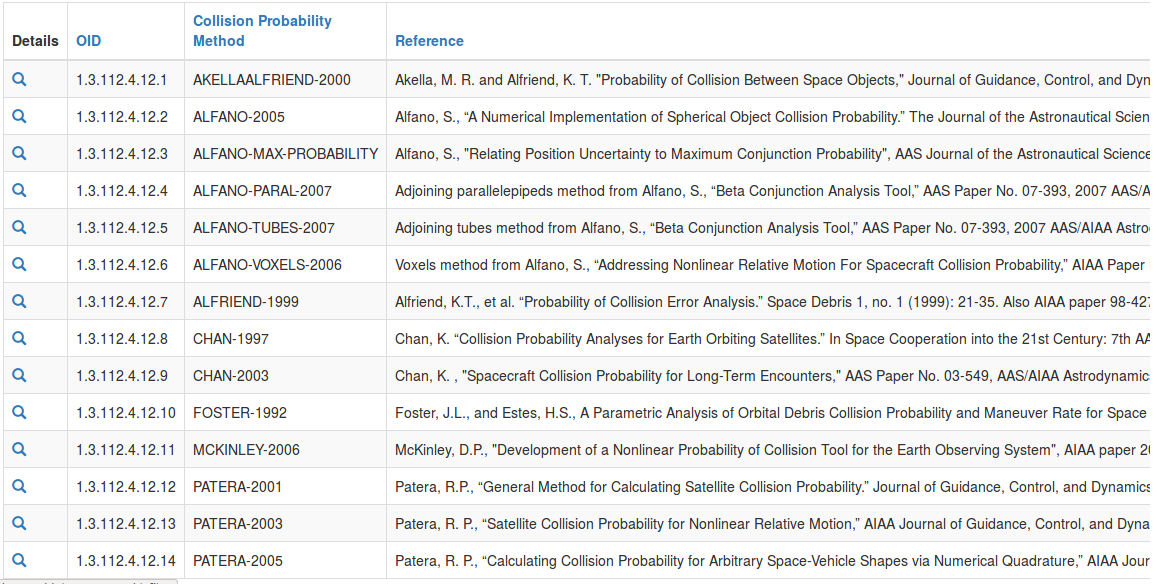
\includegraphics[width=\textwidth]{imagenes/sanaPoCmetodos}
\caption[M\'etodos de c\'alculo de PoC - (Sitio Web SANA)]{ La imagen es una impresi\'on de pantalla de la Secci\'on Probabilidad de Colisi\'on, del sitio SANA: \textcolor{blue}{http://sanaregistry.org/r/ndmxml/ndmxml-1.0-cdm-1.0.xsd}, que se indica en el est\'andar del CCSDS, para la descripci\'on de los esquemas del formato XML del CDM.}
\label{fig:pagsana}
\end{figure}

\section*{Resumen}
A partir de la recepci\'on de informaci\'on respecto de una posible colisi\'on, ya sea mediante un mensaje estandarizado CDM o mediante el ingreso manual, se inicia un an\'alisis de la situaci\'on.\\
A tal fin:\\
(Ver Fig. \ref{fig:flujomain})
\begin{itemize}
\itemsep0em
\item Se identifican los objetos involucrados, y se extra su identificador de NORAD y el TCA.
\item Se solicitan los TLE de los \'ultimos 15 d\'ias m\'as pr\'oximos a la fecha del encuentro, para el desecho y para la misi\'on operativa en caso de no contar con datos m\'as precisos. Si para la misi\'on operativa se contara con productos orbitales propios se utilizar\'an los errores calculados asociados a los mismos.
\item Se calcula la matriz de covarianza con el m\'etodo de Osweiler para el desecho (y para la misi\'on si los datos orbitales de la misma no se conocieran).
\item Se propagan ambas matrices hasta el TCA utilizando los datos estad\'isticos de la tabla generada, seg\'un la cantidad de d\'ias que se necesite propagar.
\item Se proyectan los distintos par\'ametros a un plano de encuentro que simplifica los c\'alculos.
\item Se calcula la probabilidad de colisi\'on mediante la expresi\'on aproximada de Lei-Chen.
\end{itemize}

\begin{figure}[!h]
\centering
\fbox{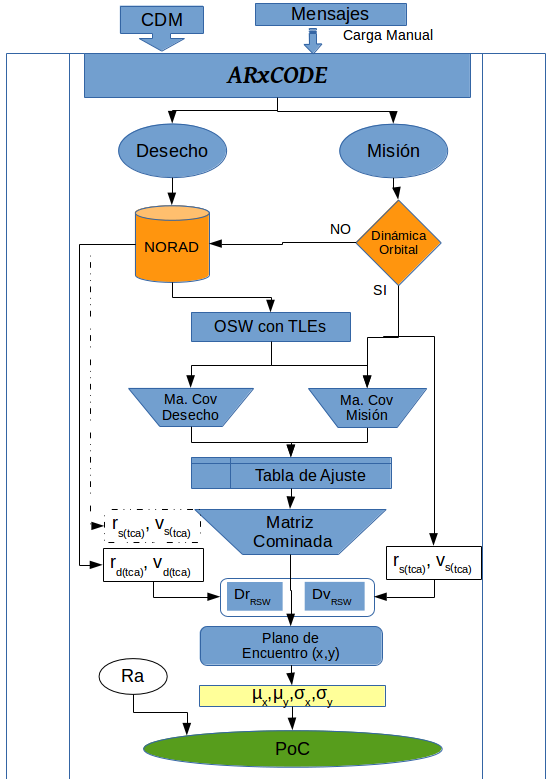
\includegraphics[width=0.7\textwidth]{imagenes/flujomain}}
\caption[Esquema del Procedimiento General del c\'alculo de PoC]{Esquema del Procedimiento General del c\'alculo de PoC}
\label{fig:flujomain}
\end{figure}

\endinput
\chapter{Metodología de Desarrollo}
\label{chap:metodologia}
%\endinput
 %De acuerdo a \cite{Barrett2009}, el modelo WCM...\\
Para el desarrollo de este trabajo se opt\'o por un modelo de desarrollo de tipo incremental (que resulta iterativo por naturaleza).
En cada iteraci\'on, se optimiz\'o el dise\~no y se fueron agregando nuevas funcionalidades y capacidades al sistema.\\

El problema que se propone resolver, requiere de la implementaci\'on de distintos algoritmos en una estructura en donde los resultados de un m\'odulo se utilizan en el siguiente. Esto implica que para un an\'alisis completo cada una de las instancias debi\'o estar previamente validada.
No obstante, las salidas de los m\'odulos que eran ingesta de otros m\'odulos pod\'ian reemplazarse por datos ya conocidos, y as\'i desarrollar y validar el m\'odulo siguiente, mientras se analizaba en paralelo c\'omo mejorar o corregir los resultados no satisfactorios. De esta manera se fue armando el cuerpo general del software a gran escala, y luego se fue revisando y afinando cada uno de los paquetes.\\

Esta forma de trabajo permiti\'o dividir la complejidad del proyecto, y a su vez, desarrollar un conjunto de bibliotecas f\'acilmente modificables, sin alterar la estructura central.\\

\section{Inicializaci\'on}
En esta primera etapa se evalu\'o  el concepto del ARxCODE en el contexto de la Unidad de Desarrollo de Desechos Espaciales de la CONAE. Fundamentalmente la vinculaci\'on con el departamento de Din\'amica Orbital y los procedimientos actuales que se realizan en relaci\'on a los riesgos de colisi\'on con desechos.

Se hizo un estudio de las estructuras org\'anicas existentes y los sistemas asociados. Los distintos tipos de productos y usuarios, las interfaces que existen y el acceso a los datos reales con los que se  podr\'ia contar.\\

Se analiz\'o c\'omo trabajan otras agencias espaciales el problema de los desechos espaciales y se sacaron conclusiones respecto de qu\'e es lo que podr\'ia ofrecerse y bajo qu\'e premisas.\\

De las consideraciones m\'as importantes que se desprendieron de esta etapa, cabe destacar que se decidi\'o un prototipo para funcionar montado sobre el software principal de Din\'amica Orbital, como un anexo que no interfiere de ninguna manera con los procesos actuales.
Por otro lado, debido a la complejidad del problema y sus consecuencias, ser\'a un software diseñado para ser utilizado por un analista experto, con conocimientos de Din\'amica Orbital.\\

En el mismo sentido, sus productos finales no ser\'an considerados en la toma de decisiones hasta tanto sus resultados no hayan sido validados durante un periodo suficiente, que permita verificar y mejorar su funcionamiento, contrast\'andolo con un acumulado de situaciones reales.\\

Para este planteo de definiciones, se cont\'o con el asesoramiento y el intercambio de informaci\'on con personas del \'area de Din\'amica Orbital y otros departamentos de la CONAE. Se realizaron algunas reuniones e intercambio de correos electr\'onicos, aunque por ser una tem\'atica que se aborda bajo reg\'imenes especiales de acuerdos de confidencialidad, no fue posible contar con la totalidad de la informaci\'on.

\section{Iteraci\'on}
Ya conocido el planteo del problema, las distintas maneras de abordarlo y las restricciones, se elabor\'o un diseño preliminar del producto con sus requerimientos (Sec. \ref{sec:requerimientos}) y sus funcionalidades, que dadas las caracter\'isticas del problema result\'o bastante determinista.\\

Para el desarrollo se definieron distintos paquetes o componentes (Sec. \ref{subsec:componentes}):\\

\begin{itemize}
\itemsep0em
 \item Paquetes de Procesamiento: {\it{AjustarTle}}, {\it{Comparar}}, {\it{Encuentro}}, {\it{Estad\'istica}}.
 \item Paquetes de Administraci\'on de Datos: {\it{TleAdmin}}, {\it{CodsAdmin}}, {\it{CDM}}.
 \item Paquetes Generales de utilizaci\'on m\'ultiple: {\it{SistReferencia}}, {\it{Validaci\'on}}.
 \item Paquetes de visualizaci\'on e interfaz gr\'afica: {\it{Aplicaci\'on}}, {\it{visual}}.
\end{itemize}

Esta metodolog\'ia permiti\'o importar funciones que resuelven cuestiones espec\'ificas desde cualquier  m\'odulo y a su vez modificar las funciones cuando fuera necesario.\\

Durante el diseño y el desarrollo de la interfaz, se fueron modificando mucho las opciones, en tanto se utiliz\'o la interfaz para seguimiento de pasos intermedios que a medida que iban siendo validados se iban retirando de las opciones del usuario.\\

\section{Control}
Al tratarse de un sistema que implementa distintas metodolog\'ias para el c\'alculo de par\'ametros, el control se bas\'o en analizar que los resultados de los algoritmos implementados fueran coherentes y coincidieran con los que exist\'ian en publicaciones bibliogr\'aficas que se pod\'ian reproducir.\\

Fue fundamental implementar un control sobre la implementaci\'on de la solicitud a NORAD y la propagaci\'on de los TLE y sobre los algoritmos de transformaci\'on de coordenadas.\\

Para cada una de las instancias de validaci\'on se configuraron distintos escenarios de prueba y en muchas oportunidades se verificaron los resultados parciales con pruebas realizadas en Microsoft Excel.\\

\section{Entorno de Desarrollo}

Para el desarrollo se utiliz\'o:\\
\begin{itemize}
 \item Plataforma de Desarrollo (\ac{IDE}): Eclipse Ver. 3.8.1.
 \item Lenguaje de Programaci\'on: Python 2.7
 \item Biblioteca de Interfaz gr\'afica: QT por medio del enlace PyQT.
 \item Gestor de Configuraci\'on: Git.
\end{itemize}

\subsection*{Eclipse}
Eclipse (Ver. 3.8.1) es una plataforma de desarrollo multiplataforma ampliamente utilizada y ya muy madura, cuya estructura de perspectivas, editores y vistas, facilita el desarrollo en distintos lenguajes de programaci\'on. En este trabajo se incorpor\'o el IDE para python, {\it{Pydev}}.\\

Eclipse ofrece excelentes capacidades para la gesti\'on de proyectos, permitiendo incorporar en un mismo proyecto distintos archivos y documentaci\'on, que, en esta tesis, agrup\'o no s\'olo los datos de entrada y salida, como los TLE, los CDM o los productos orbitales; sino que tambi\'en incluy\'o todos los ploteos y gr\'aficos que resultaban de los procesamientos y la propia documentaci\'on referida a la escritura de este documento. Esto fue muy productivo en lo que respecta al control de versiones, ya que se aprovech\'o el hecho de que Eclipse ya tiene incorporado el gestor Git.
Cabe destacar también, que cuenta con una excelente herramientas de depuraci\'on.\\

\subsection*{Python}
El lenguaje de programaci\'on Python se destaca en sus capacidades tanto de c\'alculo como de manejo de texto. Esto agiliza mucho los procesos que involucran el manejo de tablas de datos plasmadas en texto plano, como son por ejemplo los datos TLE y las efem\'erides orbitales que se generan como productos del departamento de Din\'amica Orbital. As\'i mismo facilita el manejo de las nomenclaturas de los distintos archivos de datos o im\'agenes generadas.\\

Existen numerosas, potentes y optimizadas bibliotecas para la realizaci\'on de c\'alculos, y el tratamiento vectorial. En nuestro caso se aprovech\'o particularmente la biblioteca {\it{numpy}}, y muy poco de {\it{scipy}} espec\'ificamente, para interpolar datos.
Finalmente su utilizaci\'on masiva permite tener acceso r\'apido a sus potencialidades.\\

\subsection*{QT}
Para el desarrollo de la interfaz gr\'afica se utiliz\'o QT, a trav\'es del enlace PyQT.\\
QT es un framework ampliamente utilizado para el desarrollo de aplicaciones multiplataforma. Cuenta con mucha contribuci\'on de la comunidad y est\'a soportado por Nokia.\\

Su mecanismo de conexión de señales y eventos es simple, esto permite definir los eventos sencillos en la estructura del GUI, y luego invocar el c\'odigo python con las acciones m\'as avanzadas. Subyace su implementaci\'on en C++ que muchas veces dificulta la comprensi\'on para los que estamos familiarizados con la l\'ogica del python, y lo mismo ocurre con la documentaci\'on y prevalecen los ejemplos para C++.\\

\subsection*{Git}
Si bien, esta herramienta no fue aprovechada en todo su potencial en este trabajo, por tratarse de un proyecto sencillo y desarrollada por dos personas, fue fundamental para agilizar la posibilidad de trabajar desde cualquier computadora, siempre en la \'ultima versi\'on del proyecto.
As\'i mismo, el trabajo con control de versiones, permiti\'o realizar distintas pruebas e implementaciones que luego se descartaron o se quitaron del producto final, pero que pueden ser reutilizados en futuros proyectos. En particular, en la utilizaci\'on de la interfaz intermedia que fue generada para una \'agil evaluaci\'on de los resultados parciales.\\










\chapter{ARxCODE}
\label{chap:arxcode} 

%\endinput
\section{Especificaciones generales}

ARxCODE es un prototipo de software dise\~nado para el procesamiento y an\'alisis de encuentros con riesgo de colisi\'on, entre misiones operativas y desechos espaciales.\\
Tiene como objetivo principal procesar la informaci\'on, proveniente de los organismos internacionales de alerta (mensaje CDM), o cargada manualmente, y facilitar al operador la visualizaci\'on de los par\'ametros de la situaci\'on en forma clara para su correcta interpretaci\'on y comunicaci\'on.\\
Es una aplicaci\'on de escritorio, de estructura modular, reusable y modificable que cuenta con una interfaz amigable.\\
Pensada con una filosof\'ia de expansi\'on y perfeccionamiento, su arquitectura permite la adici\'on de funcionalidades sin mayores inconvenientes.\\

% Describir:
% \begin{itemize}
% \itemsep0em
%  \item  M\'odulos Fundamentales.
%  \item Flujo de Pantallas.
%  \item Diagrama de Componentes.
%  \item Requerimientos.
%  \item Casos de USO.
%  \item Entidades (diagrama de clases)
%  \item Diagrama de Secuencia.
%  \item Dise\~no de interfaces.
% \end{itemize}

\section{Requerimientos}\label{sec:requerimientos}

Se pretende que ARxCODE sea una herramienta que oficie de soporte al operador en el di\'alogo con los organismos internacionales que proveen los mensajes de alerta, frente a una situaci\'on de riesgo de colisi\'on. A tal fin, el sistema debe tener la capacidad de interpretar los mensajes estandarizados CDM y presentar la informaci\'on que all\'i se registra, en forma clara al operador.\\
Por otro lado, debe tener la capacidad de colectar datos ingresados manualmente por el operador y ofrecer los par\'ametros que resulten del procesamiento propio del ARxCODE, como m\'inima distancia, TCA calculado y PoC.\\
Esta \'ultima funcionalidad implica que ARxCODE debe poder solicitar a la p\'agina Space-Track los TLEs correspondientes a los objetos involucrados, debe poder estimar las matrices de covarianza de ambos objetos, ya sea mediante el m\'etodo de Osweiler o incorporando efem\'erides predichas del departamento de din\'amica orbital; debe poder propagar esos errores al momento del TCA y finalmente calcular la PoC, con un error aceptable.\\
En la tabla \ref{tab:req}, se listan todos los requerimientos del sistema.\\

\begin{table}[!h]
 \resizebox{\linewidth}{!}{
 \begin{tabular}{|l|l|}
 \hline \hline
   \rowcolor{lightgray}
  Req. ID & Descripci\'on \\
  \hline \hline
  \rowcolor{lightgray}
  1 & Requerimientos FUNCIONALES\\
  \hline
  ARR-010 & ARxCODE debe calcular la probabilidad de colisi\'on de un acercamiento de riesgo.\\
  \hline
  \multirow{2}{*}{ARR-020} & ARxCODE debe  aceptar como inputs: un mensaje de alerta (CDM),o los identificadores\\
  & de NORAD de ambos objetos y el tiempo de m\'aximo acercamiento (TCA).\\
  \hline
  \multirow{2}{*}{ARR-030} & ARxCODE debe utilizar los productos orbitales de la misi\'on o realizar el mismo\\
  & procedimiento que se aplica al desecho, a la misi\'on.\\
  \hline
  ARR-040 & ARxCODE debe calcular la m\'inima distancia, total y en la coordenada radial.\\
  \hline
  ARR-050 & ARxCODE debe manipular los sistemas de referencia: TEME, TOD, VNC y RTN. \\
  \hline
  \multirow{2}{*}{ARR-060}& ARxCODE debe permitir al operador/analista experto visualizar el encuentro,\\
  & generar reportes y notificaciones.\\
  \hline
  \multirow{2}{*}{ARR-070} & ARxCODE debe extraer el set de TLEs de los objetos involucrados \\
  & de los \'ultimos 15 d\'ias anteriores al TCA.\\
  \hline
  ARR-080 & ARxCODE debe estimar los errores en la posici\'on incial del desecho y de la misi\'on opeartiva.\\
  \hline
  ARR-090 & ARxCODE debe propagar los errores de la posici\'on incial al TCA.\\
  \hline
   \rowcolor{lightgray}
  2 & Requerimientos de INTERFACES \\
  \hline
  ARR-100 & ARxCODE deber\'a permitir la carga manual de la situaci\'on de encuentro.\\
  \hline
  ARR-110 & ARxCODE deber\'a descargar los TLE de Space-Track.\\
  \hline
  ARR-120 & ARxCODE deber\'a manipular los CDM con formato xml.\\
  \hline
   \rowcolor{lightgray}
  3 & Requerimientos de RENDIMIENTO y/o PERFORMANCE\\
  \hline
  ARR-210 & ARxCODE deber\'a ofrecer el reporte de la situaci\'on en no m\'as de 1 minuto \\
  \hline
    \rowcolor{lightgray}
  4 & Requerimientos de VALIDACI\'ON \\
  \hline
  \multirow{2}{*}{ARR-300} & Los m\'odulos de implementaci\'on de metodolog\'ias de ARxCODE ser\'an validados\\
  & con los resultados de las publicaciones pertinentes y la bibliograf\'ia\\
  \hline
  ARR-310 & Las propagaciones realizadas con el SGP4 ser\'an validadas con el software STK \\
  \hline
    \rowcolor{lightgray}
  5 & Requerimientos de DISE\~NO\\
  \hline
  ARR-400 & ARxCODE tendr\'a un dise\~no modular\\
   \hline
  ARR-410 & ARxCODE se desarrollar\'a como una librer\'ia \\
  \hline
  ARR-420 & ARxCODE contar\'a con una interfaz gr\'afica \\
  \hline
    \rowcolor{lightgray}
  6 & Requerimientos de IMPLEMENTACI\'ON\\
  \hline
  ARR-500& ARxCODE ser\'a implementado en python 2.7\\
  \hline
  ARR-510& ARxCODE ser\'a implementado en el entorno de desarrollo Eclipse\\
  \hline
  ARR-520& El control de versiones se realizar\'a con Git\\
  \hline
    \rowcolor{lightgray}
  7 & Requerimientos de REUSABILIDAD\\
  \hline
  ARR-600 & ARxCODE utilizar\'a la librer\'ia de SGP4 en Python \\
  \hline
  ARR-610 & ARxCODE utilizar\'a la librer\'ia de Element Tree para el parseo del CDM\\
  \hline
  ARR-620 & ARxCODE utilizar\'a la librer\'ia de ..bla..para la conexi\'on con Space-Track\\
  \hline
  ARR-630 & ARxCODE utilizar\'a la librer\'ia de ..bla..para los c\'alculos estad\'isticos y de integraci\'on \\
  \hline
 \end{tabular}
 }
 \caption[Tabla de Requerimientos]{Tabla de especificaci\'on de requerimientos del ARxCODE}
 \label{tab:req}
\end{table}


\section{Interfaces}
ARxCODE fue pensado para ser un sistema anexo a las estructuras ya existentes dentro del departamento de Din\'amica Orbital.\\
El dise\~no completo, contempla un acceso directo al servidor de la base de datos de los productos de Din\'amica Orbital para la obtenci\'on de: las efem\'erides propagadas de la misi\'on operativa, y los mensajes de alerta (CDM). Estos \'ultimos tambi\'en podr\'an ser recibidos por mail de los organismos internacionales de alerta, como por ejemplo JSpOC o mediante una solicitud a la p\'agina Space-track, previa notificaci\'on y registro autorizado del operador a cargo. (Ver Fig. \ref{fig:interfaces})\\

\begin{figure}
\centering
  \fbox{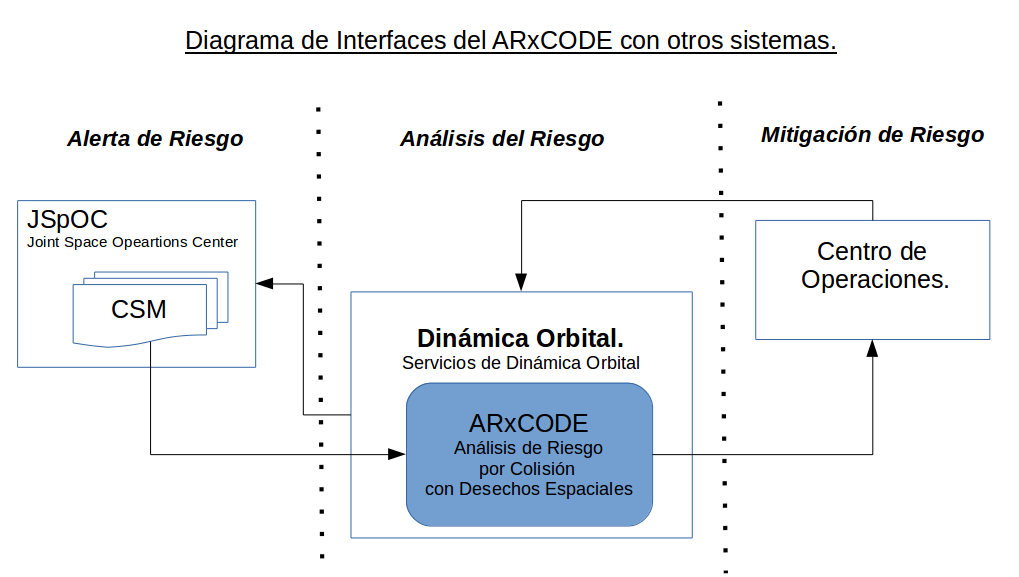
\includegraphics[width=0.8\textwidth]{imagenes/interfasessistemas}}
  \caption[Diagrama de Interfaces del Sistema]{Diagrama de Interfaces del Sistema}
  \label{fig:interfaces}
\end{figure}

No obstante, por cuestiones de tiempo y de accesibilidad, para el desarrollo de este trabajo, los datos que provee el departamento de din\'amica orbital fueron descargados y se extraen de un directorio, al igual que los mensajes de alerta CDM, que fueron descargados de pa\'aginas de internet , ya que no nos han facilitado ninguno vinculado a la misi\'on operativa de la que cual procesamos los productos orbitales, por motivos de confidencialidad. Se realiz\'o la automatizaci\'on de la descarga de TLEs de la p\'agina Space-Track y se habilit\'o en la interfaz la pantalla que permite la carga manual de los datos del encuentro.\\

En conclusi\'on, las interfaces implementadas, son (Ver Fig. \ref{fig:interfacesImpl}):\\
\begin{itemize}
\itemsep0em
 \item Conexi\'on a Space-Track para la solicitud de TLEs.
 \item Administraci\'on de las efem\'erides orbitales de los directorios de CodsAdmin.
 \item Administraci\'on de los CDM del directorio CDM, a trav\'es de la intervenci\'on del operador.
 \item Carga Manual de datos de un encuentro realizada por el operador.
\end{itemize}

\begin{figure}
\centering
  \fbox{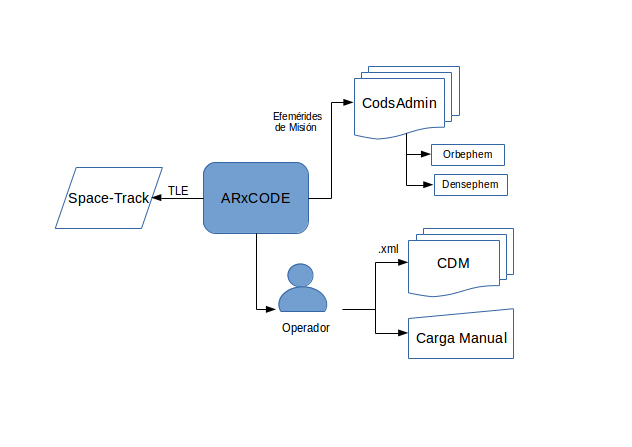
\includegraphics[width=0.8\textwidth]{imagenes/interfazImplementada}}
  \caption[Diagrama de Interfaces Implementadas en ARxCODE]{Diagrama de Interfaces Implementadas en ARxCODE}
  \label{fig:interfacesImpl}
\end{figure}

\section{Arquitectura}


\subsection*{Componentes}\label{subsec:componentes}
En un planteo conceptual, con alto grado de abstracci\'on, los distintos paquetes de ARxCODE pueden agruparse en cinco componentes Fig.  \ref{fig:componentes}: PROCESAMIENTO, ADMINISTRACI\'ON DE DATOS, INTERFAZ GR\'AFICA Y VISUALIZACI\'ON, Sistemas de Referencia y VALIDACIONES.\\

\begin{itemize}
 \item PROCESAMIENTO: Involucra los cuatro paquetes que no s\'olo operan con los datos ingresados, sino que tambi\'en los manipulan y procesan para generar nuevos productos. Estos m\'odulos son, de alguna manera los distintos n\'ucleos del c\'odigo.\\
 \begin{itemize}
 \itemsep0em
  \item {\it{AjustarTle}}
  \item {\it{Comparar}}
  \item {\it{Estadistica}}
  \item {\it{Encuentro}}
 \end{itemize}
 \item ADMINISTRACI\'ON DE DATOS: Son aquellos paquetes que se encargan de la obtenci\'on, el desgloce y el preprocesamiento de los datos que ser\'an utilizados por el resto de los m\'odulos.
 \begin{itemize}
 \itemsep0em
  \item {\it{TleAdmin}}
  \item {\it{CodsAdmin}}
  \item {\it{CDM}}
 \end{itemize}
 \item INTERFAZ Y VISUALIZACI\'ON: Agrupa el paquete que genera la interfaz gr\'afica y el paquete que contiene todos los m\'odulos que generan represntaciones visuales, como los ploteos o los tracks de las trayectorias de los objetos.\\
 \begin{itemize}
 \itemsep0em
 \item {\it{Aplicacion}}
 \item {\it{visual}}
 \end{itemize}
 \item Sistemas de Referencia: {\it{SistReferencia}}, es el paquete que contiene todo lo referente a las transformaciones entre los distintos sistemas de referencia, ya sean espaciales o de tiempo.
 \item VALIDACIONES: Agrupa todos los m\'odulos desarrollados para validar los resultados.
\end{itemize}


\begin{figure}[h!]
  \centering
  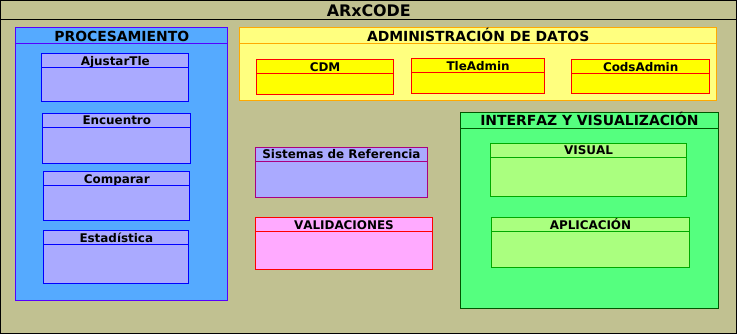
\includegraphics[width=.8\textwidth]{imagenes/componentesAR}
  \label{fig:componentes}
  \caption{Componentes de ARxCODE}
\end{figure}


\subsection{Casos de Uso}

Este trabajo se pens\'o como un adicional, o un \textcolor{red}{agregado}, al software principal del departamento de din\'amica orbital. En este sentdio, no existe gran complejidad en la estrucutura del prototipo, ya que su valor, radica en la correcta implementaci\'on de los algoritmos que procesan la informaci\'on del encuentro.\\
Identificamos dos clases de uso Fig. \ref{fig:casosuso} :\\
\begin{itemize}
 \item {\it{Procesar Encuentro}}: que nuclea el procesamiento vertebral de ARxCODE
 \item {\it{Ver informes de encuentros anteriores}}: ofrece encuentros anteriores.
\end{itemize}

\begin{figure}[h!]
  \centering
  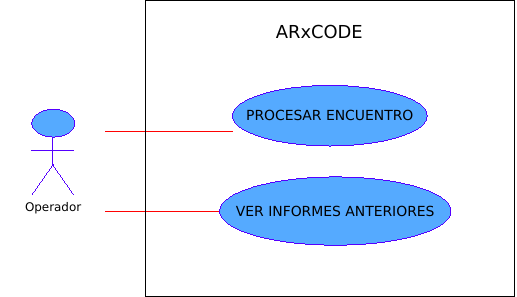
\includegraphics[width=.5\textwidth]{imagenes/usecaseAR}
  \label{fig:casosuso}
  \caption{Casos de Uso de ARxCODE}
\end{figure}


 \begin{table}[h]
\centering
\resizebox{18cm}{!}{
\begin{tabular}[c]{|l|l|}
\hline
\bf{Nombre}  &    \it{Procesar Encuentro}\\
\hline
Actor  &    Operador de Din\'amica Orbital con Autorizaci\'on\\
\hline
\multirow{ 3}{*}{Prop\'osito} & Calcular la probabilidad de colisi\'on, la m\'inima distancia total\\
& y m\'inima distancia en la coordenada radial, para poder hacer un an\'alisis\\
& de la situaci\'on de encuentro.\\
\hline
\multirow{ 4}{*}{Resumen}& Procesa la ingesta de datos de un encuentro, (CDMs o ingreso manual)\\
&  y calcula los par\'ametros de la situaci\'on de riesgo:\\
& m\'inima distancia total, m\'inima distancia en la coordenada radial y probabilidad de colisi\'on.\\
& Realiza gr\'aficos e informes.\\
\hline
Requerimientos  &    \\
\hline
\multirow{ 3}{*}{Precondiciones}  &  El operador debe estar registrado en la p\'agina space-track de NORAD.  \\
& Los archivos CDM deben estar previamente cargados en el Directorio de b\'usqueda.\\
& El operador debe conocer el encuentro que desea analizar y sus datos en caso del ingreso manual.\\
\hline
\multirow{ 3}{*}{Flujo Principal} & 1 - El operador selecciona un archivo CDM \\
& 2 - El operador oprime el bot\'on {\it{Track}} para visualizar el encuentro proyectado en la superficie terrestre (opcional)\\
& 3 - El operador oprime el bot\'on para genera un informe (opcional)\\
\hline
\multirow{ 3}{*}{Flujo Alternativo} & 1 - El operador ingresa los n\'umeros de identificaci\'on de los objetos (NORAD\_ID) \\
& 2 - El operador ingresa la fecha y hora del m\'aximo acercamiento (TCA)\\
& 3 - El operador oprime el bot\'on {\it{Procesar}} para procesar el encuentro\\
\hline
Postcondiciones & El informe de an\'alisis de riesgo fue generado y almacenado.\\
\hline
\end{tabular}}
\caption[Caso de Uso: Procesar Encuentro]{Tabla con la descripci\'on del caso de uso: \it{Procesar Encuentro}}
\label{tab:usoproceso}
\end{table}

\begin{figure}[h!]
  \centering
  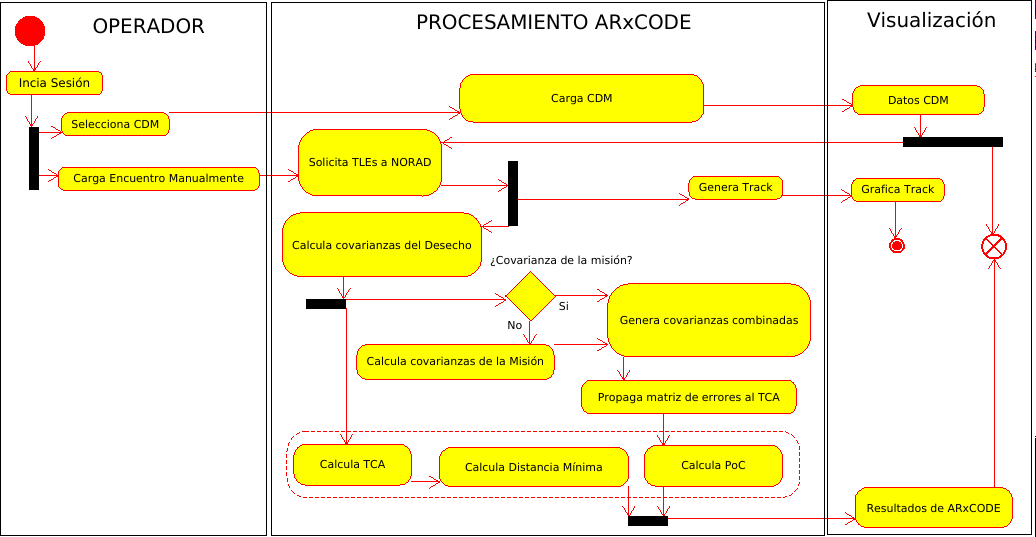
\includegraphics[width=\textwidth]{imagenes/actdiagAR}
  \label{fig:actdiag}
  \caption{Diagrama de Actividades de ARxCODE}
\end{figure}

\section{Entradas y Salidas}

archivos y demases

\subsection*{Preprocesamiento de los Datos de Misi\'on de CODS}
Para este trabajo CONAE nos facilit\'o el acceso a los datos orbitales de la misi\'on SAC-D.
Los datos se ecuentran montados en un servidor que contiene la informaci\'on organizada en archivos con formato ASCII, distribuidos en distintas carpetas seg\'un su clasificaci\'on.\\
Para la comparaci\'on que proponemos, solicitamos acceso a los archivos de efem\'erides orbitales ORBEPHEM, que ofrecen posiciones y velocidades tabuladas cada un minuto, en el Sistema de Referencia TOD (True of Date), en coordenadas cartesianas.

\subsection*{ORBEPHEM}
Estos productos son generados luego de un post procesamiento que incluye una propagaci\'on ajustada por una determinaci\'on orbital. 
Cada archivo contiene un listado cronol\'ogicamente tabulado de posiciones y velocidades, dentro de un periodo de casi 3 d\'ias. ( doc\_interfaces)

La nomenclatura de los mismos respeta el siguiente formato:\\
\begin{verbatim}
 CODS_YYYYMMDD_HHMMSS_SACD_ORBEPHEM_TOD_XYZ_O.TXT
 
 Donde:
  CODS = Identifica el Servicio dentro del CUSS que presta la información.
  YYYYMMDD_HHMMSS = epoca de generación del dato.
  SACD = Identificación del Satélite.
  ORBEPHEM = Tipo de Dato, Efeméride Orbital (procesada a posteriori)
  TOD = Sistema de Referencia True of Date.
  XYZ = Tipo de efeméride, cartesiana.
  O = Operacional. 
\end{verbatim}


\subsection*{Archivos Utilizados}
Si bien la nomenclatura de los archivos respeta una estructura, s\'olo se indica en el nombre, la fecha de generaci\'on de los datos y no puede desprenderse del mismo cu\'al es la \'epoca final e inicial de cada archivo, y no existe un registro del los gaps de datos ausentes. A su vez, las \'epocas contempladas en cada uno de ellos no está homogeneizada. Es decir, la fecha y hora inicial y final de cada registro es diferente para cada archivo.\\
Dada esta organizaci\'on, para el punto tres del procedimiento, referente a la localizaci\'on del archivo necesario para la comparaci\'on, la b\'usqueda se realiza de la siguiente manera:\\
Localizamos en primer lugar el archivo cuyo nombre coincide con la fecha de la \'epoca del TLE primario.
Como una misma fecha se encuentra en m\'as de un archivo, buscamos el archivo que contenga esa fecha y que adem\'as sea el m\'as actualizado de todos. Para ello, además del archivo cuyo nombre contiene la fecha del TLE primario, se enlistan los siguientes dos archivos y se ordenan en orden decreciente, de manera que el primer lugar de la lista lo ocupe el \'ultimo de los archivos seleccionados. Finalmente se comienza el proceso iterativo de abrir los archivos, evaluar el contenido y ver si se encuentran los dos registros que encierren la \'epoca del TLE.
Una vez que se encuentran las l\'ineas de efem\'erides que contienen la \'epoca de inter\'es se interpola, y se termina la iteraci\'on.

\noindent
Cantidad TOTAL de archivos $=  1454$\\
Cantidad media de resgistros por archivo $=  2688$\\
Archivo con el mayor n\'umero de registros $=  3042$\\
Archivo con el menor n\'umero de registros $=  142$\\


\section*{Diferencias}

\begin{itemize}
 \item Revisar escritura sobre datos CODS.
 \item Comparar defasaje inicial con defasaje de TLE respecto de GPS. (ver tendencias - empezar a diagramar los apédices)
 \item Comparar errores lineal vs cuadr\'atico.
\end{itemize}

\chapter{Resultados}
\label{chap:resultados}

\section{validacion}

Dado que la salida del SGP4 ofrece las coordenadas en el sistema TEME, y que los datos provistos
por CODS est\'an publicados en el sistema TOD, hicimos un m\'odulo de transformaci\'on que validamos
utilizando el software STK.\\
Se detallan a continuaci\'on los resultados en ambos softwares y se verifica que las diferencias son peque\~nas, 
alcanzando m\'aximos del orden de cent\'imetros.\\

Salida ARxCODE.\\

\begin{tabular}{lcccccc}
2012-05-25 00:00& 6123.226358& -2799.6061073& 2030.22212402& 1.509737& -1.894738& -7.130677\\
2012-05-25 00:01& 6201.109925& -2907.4340358& 1598.47477776& 1.085502& -1.698287& -7.255920\\
2012-05-25 00:02& 6253.396906& -3003.2608146& 1160.11171533& 0.656815& -1.494839& -7.351125\\
2012-05-25 00:03& 6279.873805& -3086.6920159& 716.947643232& 0.225465& -1.285245& -7.415900\\
2012-05-25 00:04& 6280.434799& -3157.3849876& 270.816930972& -0.20674& -1.07038& -7.449981\\
2012-05-25 00:05& 6255.082153& -3215.0502978& -176.43422104& -0.63802& -0.85114& -7.453239
\end{tabular}

Salida STK.\\

\begin{tabular}{lcccccc}
25 May 2012 00:00& 6123.226382& -2799.605966& 2030.222245& 1.509738& -1.894738& -7.130677\\
25 May 2012 00:01& 6201.109963& -2907.433903& 1598.474875& 1.085502& -1.698287& -7.255921\\
25 May 2012 00:02& 6253.396954& -3003.260689& 1160.111787& 0.656816& -1.494840& -7.351126\\
25 May 2012 00:03& 6279.873859& -3086.691896& 716.947689&  0.225466& -1.285246& -7.415901\\
25 May 2012 00:04& 6280.434856& -3157.384873& 270.816951& -0.206748& -1.070381& -7.449982\\
25 May 2012 00:05& 6255.082210& -3215.050188& -176.434228& -0.638022& -0.851142& -7.453238
\end{tabular}





 \chapter{Conclusiones}
\label{chap:conclusiones}

En esta tesis se analiz\'o la problem\'atica de los desechos espaciales, con foco central en los riesgos de colisi\'on con misiones operativas. El estudio de un acercamiento de riesgo o encuentro, se basa en los resultados de las propagaciones orbitales de las posiciones de los objetos, cuyos errores no siempre son conocidos.\\

Conocer los errores en las posiciones es fundamental para el c\'alculo de la PoC, que es el par\'ametro actualmente aceptado para la clasificaci\'on del peligro o la toma de decisiones, como por ejemplo realizar una maniobra evasiva.\\ En este trabajo, para determinar las posiciones orbitales de los objetos se utilizaron los TLE p\'ublicos de la p\'agina Space-track, que no ofrece los errores asociados y el propagador SGP4 \citep{sgp4python} que tampoco da informaci\'on de los errores de propagaci\'on que introduce.\\

En ese sentido, a fin de mejorar la caracterizaci\'on de la situaci\'on de encuentro, se implement\'o el m\'etodo de Osweiler \citep{osweiler} para la estimaci\'on de las matrices de error de las posiciones de los objetos, y se utilizaron efem\'erides precisas para la elaboraci\'on de una tabla que contiene los valores de los errores propagados en funci\'on de los d\'ias de propagaci\'on.\\

Los resultados indican que la construcci\'on de las matrices de error se realiza correctamente, no obstante, los valores que arroja el m\'etodo son muy grandes y absorben los resultados encontrados para la matriz de propagaci\'on propuesta, impidiendo una mejora en la determinaci\'on de la posici\'on.  A su vez, el c\'alculo de la PoC es muy sensible a los valores de las matrices de covarianza, por lo que resulta insuficiente considerar las mejoras en la determinaci\'on de la propagaci\'on.\\

Para el c\'alculo de la PoC se estudiaron distintos m\'etodos, y se opt\'o por la expresi\'on simplificada que considera \'orbitas circulares que describe Lei-Chen \citep{leichen}. Puede observarse que esta expresi\'on resulta muy sensible a los errores de las posiciones de los objetos y al radio de colisi\'on seleccionado. As\'i, los resultados obtenidos en este trabajo, podr\'ian coincidir perfectamente con los datos publicados en el libro de  Klinkrad, \citep{Klinkrad} o con los resultados de Xi y Xiong \citep{xu2014method}), variando los valores del radio de colisi\'on, para aquellos casos en los que los errores en las posiciones no son muy grandes.

Con el objeto de incorporar todos estos c\'alculos a un procedimiento operativo frente a situaciones de riesgo de colisi\'on, se desarroll\'o un prototipo de software: ARxCODE, que recibe alertas de posibles colisiones en el formato estandarizado CDM o bien por ingreso manual del operador, y devuelve: el TCA, la m\'inima distancia entre objetos, la PoC y la proyecci\'on de las \'orbitas sobre la superficie de la Tierra; todo en una aplicaci\'on con una interfaz amigable; para dar soporte a los operadores en las situaciones de riesgo. 

ARxCODE fue pensado para operar montado sobre las estructuras ya existentes del departamento de Din\'amica Orbital y para ser utilizado por operadores o analistas con alto conocimiento sobre din\'amica orbital y desechos espaciales.\\

Entre sus funcionalidades principales, ARxCODE:\\

\begin{itemize}
 \item Extrae la informaci\'on que contienen los mensajes de alerta estandarizados CDM, y publica por pantalla: la {\it{m\'inima distancia}}, la {\it{probabilidad de colisi\'on}} y el {\it{tiempo de m\'aximo acercamiento}} (TCA). 
 \item Implementa el m\'etodo de Osweiler \citep{osweiler} para determinar las matrices de covarianza de los errores, en la posici\'on inicial.
 \item Implementa un m\'etodo desarrollado en esta tesis, para propagar las matrices de covarianza de errores hasta el TCA.
 \item Calcula la probabilidad de colisi\'on del encuentro.
 \item Grafica las trayectorias de los objetos durante el encuentro.
\end{itemize}


\section*{Trabajo a Futuro}

En este trabajo se logr\'o abarcar todo el recorrido desde un mensaje de alerta hasta la caracterizaci\'on de la situaci\'on del riesgo de una situaci\'on de encuentro; resultando en un prototipo software, con una interfaz amigable, pensado para ser utilizado por un operador con conocimientos de Din\'amica Orbital; no obstante, es necesario profundizar e incluso mejorar algunas de las instancias intermedias de la cadena de procesamiento, a fin de lograr resultados m\'as precisos y confiables; as\'i como una estructura que permita una implementaci\'on m\'as robusta con los datos que administra el departamento de Din\'amica Orbital\\

En primera instancia ser\'a necesario utilizar otros mecanimos o ajustar el m\'etodo propuesto para la determinaci\'on del error en la posici\'on inicial de los objetos. Entre las opciones que se han analizado, existe la posibilidad de incorporar una correcci\'on de ajuste a la posici\'on inicial que se utiliza en el c\'alculo del m\'etodo de Osweiler; esta correcci\'on se desprender\'ia de procesamientos previos que utilizan efem\'erides precisas. Ya se han realizado algunas pruebas, pero los resultados no fueron concluyentes, por lo que ser\'a necesario seguir evaluando de qu\'e modo impartir esa primera correcci\'on para esta idea.

Otra opción ..considerar un propagador preciso.


ARxCODE se pens\'o con una filosof\'ia de ampliaci\'on con el objeto de ir perfeccion\'andose con la propia experiencia en su utilizaci\'on. En este sentido, muchas de las pruebas e implementaciones no pudieron ser desarrolladas o validadas ya que por falta de tiempo o pol\'iticas de confidencialidad, no pudo tenerse acceso a cierta informaci\'on de interfaces o datos de situaciones reales.\\

, y validaciones con el acumulado de situaciones reales. No obstante, la imposibilidad  los datos puntuales de situaciones reales, dificult\'o las pr\'acticas de validaci\'on y muchas propuestas y desarrollos fueron descartados para ser abordados en un futuro.\\

de tener un mayor acceso a la din\'amica de las operaciones y ... la l\'ogica de las interfaces y la articulaci\'on de la recepeci\'on de los mensajes de alerta. 

\begin{itemize}
 \item Incorporar un ajuste que mejore la estimaci\'on de errores de las posiciones iniciales. 
 \item Incorporar al dise\~no una base de datos para los registros espec\'ificos de los CDM y los informes de alerta, o bien 
 crear la entidad asociada, dentro de la base existente en Din\'amica Orbital.
 \item Incorporar otros m\'etodos para el c\'alculo de la PoC.
\end{itemize}


\endinput

\bibliografia{template_tesis_mdiae.bib}

%------------------------------------------------------------------------------
% EN CASO DE TENER APÉNDICES, DESCOMENTAR A CONTINUACIÓN
% \appendix
% \chapter{Ap\'endice}
\section{Appendix 1: Transformaci\'on de Coordenadas}
\label{App1}

%[Montenbruck, Vallado Revisitin, Vallado Coorde Sys, tabla de Boado]

Para la comparaci\'on de las posiciones en coordenadas cartesianas, es necesario llevar ambos vectores a un mismo sistema de referencia.
La figura (ref) muestra un resumen de los distintos sistemas y las consideraciones de cada uno. 

\begin{figure}[!h]
  \centering
  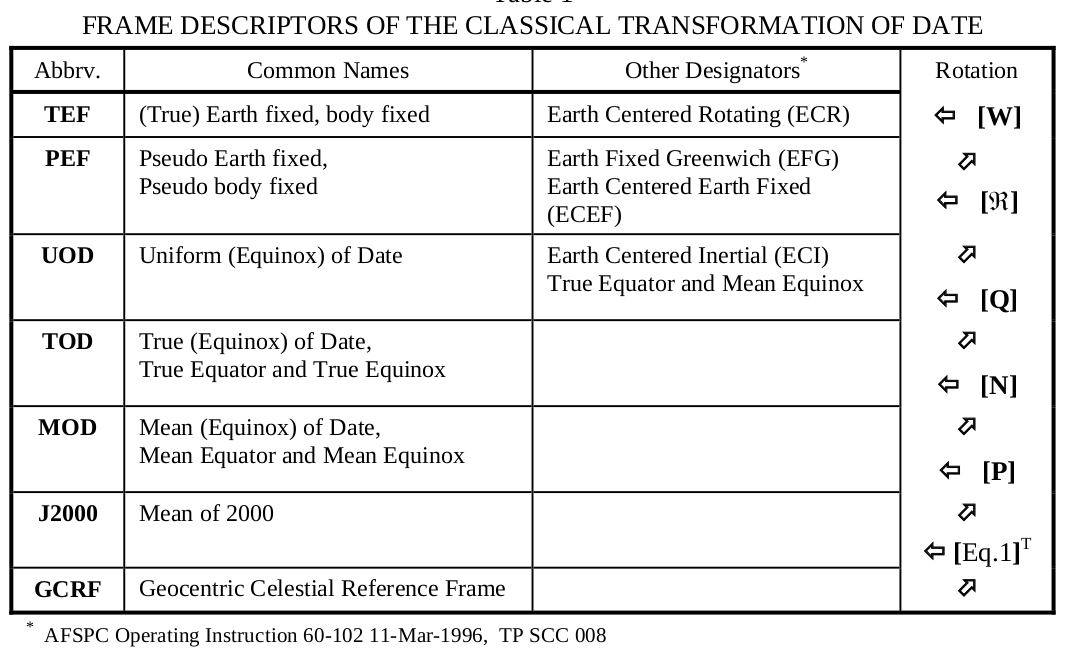
\includegraphics[width=0.7\textwidth]{imagenes/sistReferencias}
\end{figure}

En nuestro caso en particular, los datos que provee CODS se publican en el sistema TOD: True of Date (Verdadero de la \'epoca), mientras que los vectores de estado que genera el propagador SGP4 est\'an calculados en el sistema TEME: True Equator Mean Equinox (Ecuador Verdadero y Equinoccio Medio), tambi\'en denominado UOD (Uniform Equinox of Date).

Para la transformaci\'on de los datos de salida del SGP4 en el sistema TEME, al sistema TOD utilizamos la ecuaci\'on de los equinoccios, $EQ_{equinox}$, que nos permite transformar el equinoccio medio en el equinoccio verdadero.\\
Dado el vector de estado en el sistema TEME, $r_{_{TEME}}$, lo multiplicamos por la matriz de transformaci\'on en el eje z $Rot_{3}(EQ_{equinox})$ y obtenemos el vector de estado en el sistema TOD, $r_{_{TOD}}$.

\begin{equation}
 r_{_{TOD}} = [Q] r_{_{TEME}}
\end{equation}


 \[ Q =
\left( \begin{array}{ccc}
 cos(-EQ_{eqe}) & sin(-EQ_{eqe}) &  0 \\ 
 -sin(-EQ_{eqe}) & cos(-EQ_{eqe}) &  0 \\
 0 & 0 & 1
\end{array} \right) \] 


La ecuaci\'on de los equinoccios utiliza el modelo de nutaci\'on IAU-80 que considera los par\'ametros de nutaci\'on y los 106 coeficientes de Delaunay para el c\'alculo de la longitud $\Delta \Psi$ y la oblicuidad $\Delta \epsilon$.

\begin{equation}
 EQ_{eqe}=\Delta \Psi cos({\epsilon}) + 0.00264 \textquotedbl sin(\Omega_{(}) + 0.000063 \textquotedbl sin (2 \Omega_{(})
\end{equation}

Donde:

\begin{align*}
 \epsilon &= {\bar{\epsilon}} + \Delta \epsilon\\
 \Delta \Psi &= \sum_{i=1}^{106}  (A_{p} + A_{pl} tt) sin(a_{p_{i}})\\
 \Delta \epsilon &= \sum_{i=1}^{106}  (A_{e} + A_{el} tt) cos(a_{p_{i}})
\end{align*}

\begin{align*}
tt &=(jd-2451544.5)/36525.0 \\
 {\bar{\epsilon}} &= 84381.448 \textquotedbl - 46.8150 \textquotedbl tt - 0.00059 \textquotedbl tt^{2} + 0.001813 tt^{3}\\
 a_{p_{i}} &= a_{n1}M_{(}+a_{n2}M_{o}+a_{n3}\mu_{(}+a_{n4}D_{o}+a_{n5}\Omega_{(}
\end{align*}

Los coeficientes: $A_{p}$,$A_{pl}$,$A_{e}$,$A_{el}$,$a_{n_{i}}$ se extraen de la tabla de coeficientes de nutaci\'on de Seidelman, del libro de  \citep{montenbruck2012satellite}.

Y el resto de los par\'ametros se calcula seg\'un las expresiones:\\

\begin{align*}
    M_{(} &  = 134.96340251+1717915923.2178 tt+31.8792 tt^{2}+0.051 tt^{3}\\
    M_{o} & = 357.52910918+129596581.0481 tt-0.5532 tt^{2}-0.000136 tt^{3}\\
    \mu_{(} &= 93.27209062+1739527262.8478 tt-12.7512 tt^{2}-0.00103 tt^{3}\\
    D_{o} & = 297.85019547+1602961601.2090 tt-6.3706 tt^{2}+0.06593 tt^{3}\\
    \Omega_{(} & = 125.04455501-6962890.2665 tt+7.4722 tt^{2}+0.007702tt^{3}
\end{align*}

% \begin{figure}[!h]
%   \centering
%   \includegraphics[width=\textwidth]{imagenes/tablanutacion}
%   \caption{Teor\'ia de Nutaci\'on - \ac{IAU} 1980 - Tabla extra\'ida del libro de \citep{montenbruck2012satellite}}
%   \label{fig:tablaseidelman}
% \end{figure}

\newpage
%%%%%%%%%%%%%%%%%%%%%%%%%%%%%%%%
\section{Appendix 2: El archivo CDM}
\label{App2}

\lstset{language=XML,basicstyle=\small}
\begin{lstlisting}
<?xml version="1.0" encoding="UTF-8"?>
<cdm xmlns:xsi="http://www.w3.org/2001/XMLSchema-instance"
xsi:noNamespaceSchemaLocation="http://sanaregistry.org/r/ndmxml/ndmxml-1.0-master.xsd"
id="CCSDS_CDM_VERS" version="1.0">
<header>
<COMMENT>Sample CDM - XML version</COMMENT>
<CREATION_DATE>2010-03-12T22:31:12.000</CREATION_DATE>
<ORIGINATOR>JSPOC</ORIGINATOR>
<MESSAGE_FOR>SATELLITE A</MESSAGE_FOR>
<MESSAGE_ID>20111371985</MESSAGE_ID>
</header>
<body>
<relativeMetadataData>
  <COMMENT>Relative Metadata/Data</COMMENT>
  <TCA>2010-03-13T22:37:52.618</TCA>
  <MISS_DISTANCE units="m">715</MISS_DISTANCE>
  <RELATIVE_SPEED units="m/s">14762</RELATIVE_SPEED>
  <relativeStateVector>
    <RELATIVE_POSITION_R units="m">27.4</RELATIVE_POSITION_R>
    <RELATIVE_POSITION_T units="m">-70.2</RELATIVE_POSITION_T>
    <RELATIVE_POSITION_N units="m">711.8</RELATIVE_POSITION_N>
    <RELATIVE_VELOCITY_R units="m/s">-7.2</RELATIVE_VELOCITY_R>
    <RELATIVE_VELOCITY_T units="m/s">-14692.0</RELATIVE_VELOCITY_T>
    <RELATIVE_VELOCITY_N units="m/s">-1437.2</RELATIVE_VELOCITY_N>
  </relativeStateVector>
  <START_SCREEN_PERIOD>2010-03-12T18:29:32.212</START_SCREEN_PERIOD>
  <STOP_SCREEN_PERIOD>2010-03-15T18:29:32.212</STOP_SCREEN_PERIOD>
  <SCREEN_VOLUME_FRAME>RTN</SCREEN_VOLUME_FRAME>
  <SCREEN_VOLUME_SHAPE>ELLIPSOID</SCREEN_VOLUME_SHAPE>
  <SCREEN_VOLUME_X units="m">200</SCREEN_VOLUME_X>
  <SCREEN_VOLUME_Y units="m">1000</SCREEN_VOLUME_Y>
  <SCREEN_VOLUME_Z units="m">1000</SCREEN_VOLUME_Z>
  <SCREEN_ENTRY_TIME>2010-03-13T20:25:43.222</SCREEN_ENTRY_TIME>
  <SCREEN_EXIT_TIME>2010-03-13T23:44:29.324</SCREEN_EXIT_TIME>
  <COLLISION_PROBABILITY>4.835E-05</COLLISION_PROBABILITY>
  <COLLISION_PROBABILITY_METHOD>FOSTER-1992</COLLISION_PROBABILITY_METHOD>
</relativeMetadataData>
<segment>
  <metadata>
    <COMMENT>Object1 Metadata</COMMENT>
    <OBJECT>OBJECT1</OBJECT>
    <OBJECT_DESIGNATOR>12345</OBJECT_DESIGNATOR>
    <CATALOG_NAME>SATCAT</CATALOG_NAME>
    <OBJECT_NAME>SATELLITE A</OBJECT_NAME>
    <INTERNATIONAL_DESIGNATOR>1997-030E</INTERNATIONAL_DESIGNATOR>
    <OBJECT_TYPE>PAYLOAD</OBJECT_TYPE>
    <OPERATOR_CONTACT_POSITION>OSA</OPERATOR_CONTACT_POSITION>
    <OPERATOR_ORGANIZATION>EUMETSAT</OPERATOR_ORGANIZATION>
    <OPERATOR_PHONE>+49615130312</OPERATOR_PHONE>
    <OPERATOR_EMAIL>JOHN.DOE@SOMEWHERE>NET</OPERATOR_EMAIL>
    <EPHEMERIS_NAME>EPHEMERIS SATELLITE A</EPHEMERIS_NAME>
    <COVARIANCE_METHOD>CALCULATED</COVARIANCE_METHOD>
    <MANEUVERABLE>YES</MANEUVERABLE>
    <REF_FRAME>EME2000</REF_FRAME>
    <GRAVITY_MODEL>EGM-96: 36D 36O</GRAVITY_MODEL>
    <ATMOSPHERIC_MODEL>JACCHIA 70 DCA</ATMOSPHERIC_MODEL>
    <N_BODY_PERTURBATIONS>MOON,SUN</N_BODY_PERTURBATIONS>
    <SOLAR_RAD_PRESSURE>NO</SOLAR_RAD_PRESSURE>
    <EARTH_TIDES>NO</EARTH_TIDES>
    <INTRACK_THRUST>NO</INTRACK_THRUST>
  </metadata>
  <data>
    <COMMENT>Object1 Data</COMMENT>
    <odParameters>
    <COMMENT>Object1 OD Parameters</COMMENT>
    <TIME_LASTOB_START>2010-03-12T02:14:12.746</TIME_LASTOB_START>
    <TIME_LASTOB_END>2010-03-12T02:14:12.746</TIME_LASTOB_END>
    <RECOMMENDED_OD_SPAN units="d">7.88</RECOMMENDED_OD_SPAN>
    <ACTUAL_OD_SPAN units="d">5.50</ACTUAL_OD_SPAN>
    <OBS_AVAILABLE>592</OBS_AVAILABLE>
    <OBS_USED>59</OBS_USED>
    <TRACKS_AVAILABLE>123</TRACKS_AVAILABLE>
    <TRACKS_USED>119</TRACKS_USED>
    <RESIDUALS_ACCEPTED units="%" >97.8</RESIDUALS_ACCEPTED>
    <WEIGHTED_RMS>0.864</WEIGHTED_RMS>
    </odParameters>
    <additionalParameters>
    <COMMENT>Object 1 Additional Parameters</COMMENT>
    <AREA_PC units="m**2">5.2</AREA_PC>
    <MASS units="kg">2516</MASS>
    <CD_AREA_OVER_MASS units="m**2/kg">0.045663</CD_AREA_OVER_MASS>
    <CR_AREA_OVER_MASS units="m**2/kg">0.000000</CR_AREA_OVER_MASS>
    <THRUST_ACCELERATION units="m/s**2">0.0</THRUST_ACCELERATION>
    <SEDR units="W/kg">4.54570E-05</SEDR>
    </additionalParameters>
    <stateVector>
      <COMMENT>Object1 State Vector</COMMENT>
      <X units="km">2570.097065</X>
      <Y units="km">2244.654904</Y>
      <Z units="km">6281.497978</Z>
      <X_DOT units="km/s">4.418769571</X_DOT>
      <Y_DOT units="km/s">4.833547743</Y_DOT>
      <Z_DOT units="km/s">-3.526774282</Z_DOT>
    </stateVector>
    <covarianceMatrix>
      <COMMENT>Object1 Covariance in the RTN Coordinate Frame </COMMENT>
      <CR_R units="m**2">4.142E+01</CR_R>
      <CT_R units="m**2">-8.579E+00</CT_R>
      <CT_T units="m**2">2.533E+03</CT_T>
      <CN_R units="m**2">-2.313E+01</CN_R>
      <CN_T units="m**2">1.336E+01</CN_T>
      <CN_N units="m**2">7.098E+01</CN_N>
      <CRDOT_R units="m**2/s">2.520E-03</CRDOT_R>
      <CRDOT_T units="m**2/s">-5.476E+00</CRDOT_T>
      <CRDOT_N units="m**2/s">8.626E-04</CRDOT_N>
      <CRDOT_RDOT units="m**2/s**2">5.744E-03</CRDOT_RDOT>
      <CTDOT_R units="m**2/s">-1.006E-02</CTDOT_R>
      <CTDOT_T units="m**2/s">4.041E-03</CTDOT_T>
      <CTDOT_N units="m**2/s">-1.359E-03</CTDOT_N>
      <CTDOT_RDOT units="m**2/s**2">-1.502E-05</CTDOT_RDOT>
      <CTDOT_TDOT units="m**2/s**2">1.049E-05</CTDOT_TDOT>
      <CNDOT_R units="m**2/s">1.053E-03</CNDOT_R>
      <CNDOT_T units="m**2/s">-3.412E-03</CNDOT_T>
      <CNDOT_N units="m**2/s">1.213E-02</CNDOT_N>
      <CNDOT_RDOT units="m**2/s**2">-3.004E-06</CNDOT_RDOT>
      <CNDOT_TDOT units="m**2/s**2">-1.091E-06</CNDOT_TDOT>
      <CNDOT_NDOT units="m**2/s**2">5.529E-05</CNDOT_NDOT>
    </covarianceMatrix>
  </data>
</segment>
<segment>
  <metadata>
    <COMMENT>Object2 Metadata</COMMENT>
    <OBJECT>OBJECT2</OBJECT>
    <OBJECT_DESIGNATOR>30337</OBJECT_DESIGNATOR>
    <CATALOG_NAME>SATCAT</CATALOG_NAME>
    <OBJECT_NAME>FENGYUN 1C DEB</OBJECT_NAME>
    <INTERNATIONAL_DESIGNATOR>1999-025AA</INTERNATIONAL_DESIGNATOR>
    <OBJECT_TYPE>DEBRIS</OBJECT_TYPE>
    <EPHEMERIS_NAME>NONE</EPHEMERIS_NAME>
    <COVARIANCE_METHOD>CALCULATED</COVARIANCE_METHOD>
    <MANEUVERABLE>NO</MANEUVERABLE>
    <REF_FRAME>EME2000</REF_FRAME>
    <GRAVITY_MODEL>EGM-96: 36D 36O</GRAVITY_MODEL>
    <ATMOSPHERIC_MODEL>JACCHIA 70 DCA</ATMOSPHERIC_MODEL>
    <N_BODY_PERTURBATIONS>MOON,SUN</N_BODY_PERTURBATIONS>
    <SOLAR_RAD_PRESSURE>YES</SOLAR_RAD_PRESSURE>
    <EARTH_TIDES>NO</EARTH_TIDES>
    <INTRACK_THRUST>NO</INTRACK_THRUST>
  </metadata>
    <data>
    <COMMENT>Object2 Data</COMMENT>
    <odParameters>
    <COMMENT>Object2 OD Parameters</COMMENT>
    <TIME_LASTOB_START>2010-03-12T01:14:12.746</TIME_LASTOB_START>
    <TIME_LASTOB_END>2010-03-12T03:14:12.746</TIME_LASTOB_END>
    <RECOMMENDED_OD_SPAN units="d">2.63</RECOMMENDED_OD_SPAN>
    <ACTUAL_OD_SPAN units="d">2.63</ACTUAL_OD_SPAN>
    <OBS_AVAILABLE>59</OBS_AVAILABLE>
    <OBS_USED>58</OBS_USED>
    <TRACKS_AVAILABLE>15</TRACKS_AVAILABLE>
    <TRACKS_USED>15</TRACKS_USED>
    <RESIDUALS_ACCEPTED units="%" >97.8</RESIDUALS_ACCEPTED>
    <WEIGHTED_RMS>0.864</WEIGHTED_RMS>
    </odParameters>
    <additionalParameters>
    <COMMENT>Object2 Additional Parameters</COMMENT>
    <COMMENT>Apogee Altitude=768 km</COMMENT>
    <COMMENT>Perigee Altitude=414 km</COMMENT>
    <COMMENT>Inclination=98.8 deg</COMMENT>
    <AREA_PC units="m**2">0.9</AREA_PC>
    <CD_AREA_OVER_MASS units="m**2/kg">0.118668</CD_AREA_OVER_MASS>
    <CR_AREA_OVER_MASS units="m**2/kg">0.075204</CR_AREA_OVER_MASS>
    <THRUST_ACCELERATION units="m/s**2">0.0</THRUST_ACCELERATION>
    <SEDR units="W/kg">5.40900E-03</SEDR>
    </additionalParameters>
    <stateVector>
      <COMMENT>Object2 State Vector</COMMENT>
      <X units="km">2569.540800</X>
      <Y units="km">2245.093614</Y>
      <Z units="km">6281.599946</Z>
      <X_DOT units="km/s">-2.888612500</X_DOT>
      <Y_DOT units="km/s">-6.007247516</Y_DOT>
      <Z_DOT units="km/s">3.328770172</Z_DOT>
    </stateVector>
    <covarianceMatrix>
      <COMMENT>Object2 Covariance in the RTN Coordinate Frame</COMMENT>
      <CR_R units="m**2">1.337E+03</CR_R>
      <CT_R units="m**2">-4.806E+04</CT_R>
      <CT_T units="m**2">2.492E+06</CT_T>
      <CN_R units="m**2">-3.298E+01</CN_R>
      <CN_T units="m**2">-7.5888E+02</CN_T>
      <CN_N units="m**2">7.105E+01</CN_N>
      <CRDOT_R units="m**2/s">2.591E-03</CRDOT_R>
      <CRDOT_T units="m**2/s">-4.152E-02</CRDOT_T>
      <CRDOT_N units="m**2/s">-1.784E-06</CRDOT_N>
      <CRDOT_RDOT units="m**2/s**2">6.886E-05</CRDOT_RDOT>
      <CTDOT_R units="m**2/s">-1.016E-02</CTDOT_R>
      <CTDOT_T units="m**2/s">-1.506E-04</CTDOT_T>
      <CTDOT_N units="m**2/s">1.637E-03</CTDOT_N>
      <CTDOT_RDOT units="m**2/s**2">-2.987E-06</CTDOT_RDOT>
      <CTDOT_TDOT units="m**2/s**2">1.059E-05</CTDOT_TDOT>
      <CNDOT_R units="m**2/s">4.400E-03</CNDOT_R>
      <CNDOT_T units="m**2/s">8.482E-03</CNDOT_T>
      <CNDOT_N units="m**2/s">8.633E-05</CNDOT_N>
      <CNDOT_RDOT units="m**2/s**2">-1.903E-06</CNDOT_RDOT>
      <CNDOT_TDOT units="m**2/s**2">-4.594E-06</CNDOT_TDOT>
      <CNDOT_NDOT units="m**2/s**2">5.178E-05</CNDOT_NDOT>
    </covarianceMatrix>
  </data>
</segment>
</body>
</cdm>
\endinput
\end{lstlisting}

\newpage
%%%%%%%%%%%%%%%%%%%%%%%%%%%%%%%%
\section{Appendix 3: Gr\'aficos de las probabilidades de colisi\'on}
\label{App3}

Gr\'aficos con las PoC en funci\'on del radio de colisi\'on elegido. 
Resultados de las situaciones que analizan en su trabajo Xu y Xiong (\citep{xu2014method}).


\begin{figure}[!h]
  \centering
  \fbox{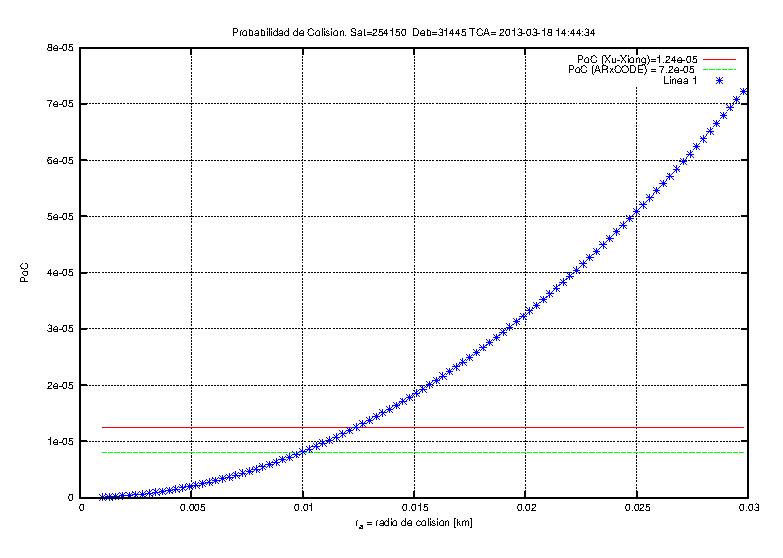
\includegraphics[width=0.6\textwidth]{imagenes/xuxiong1}}
  \caption{An\'alisis de la Probabilidad de Colisi\'on en funci\'on del radio de colisi\'on}
  \label{fig:pocvsraEsc4}
\end{figure}

\begin{figure}[!h]
  \centering
  \fbox{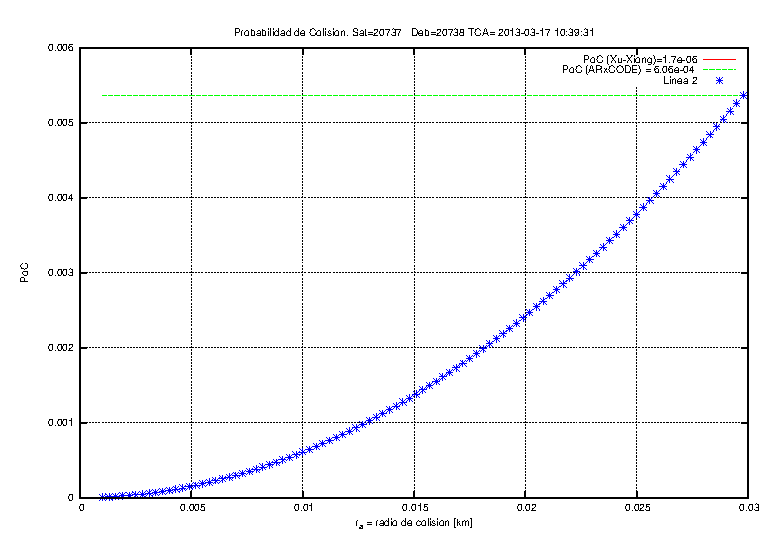
\includegraphics[width=0.6\textwidth]{imagenes/xuxiong2}}
  \caption{An\'alisis de la Probabilidad de Colisi\'on en funci\'on del radio de colisi\'on}
  \label{fig:pocvsraEsc5}
\end{figure}

\begin{figure}[!h]
  \centering
  \fbox{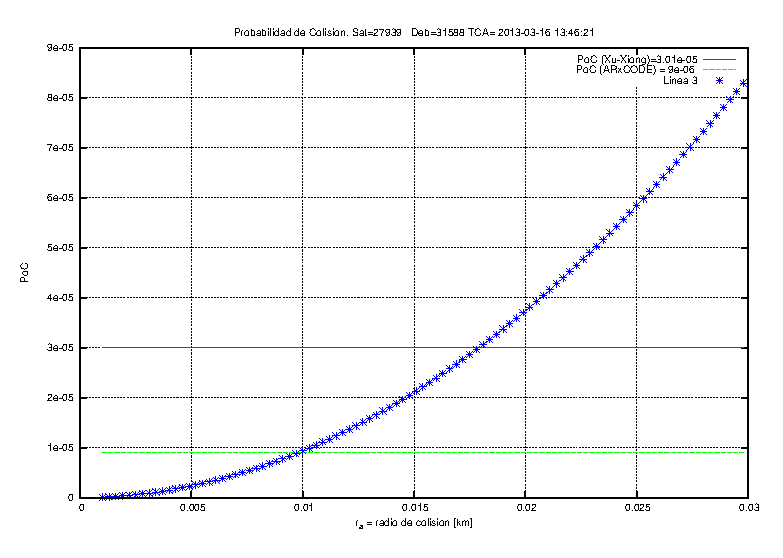
\includegraphics[width=0.6\textwidth]{imagenes/xuxiong3}}
  \caption{An\'alisis de la Probabilidad de Colisi\'on en funci\'on del radio de colisi\'on}
  \label{fig:pocvsraEsc4}
\end{figure}

\begin{figure}[!h]
  \centering
  \fbox{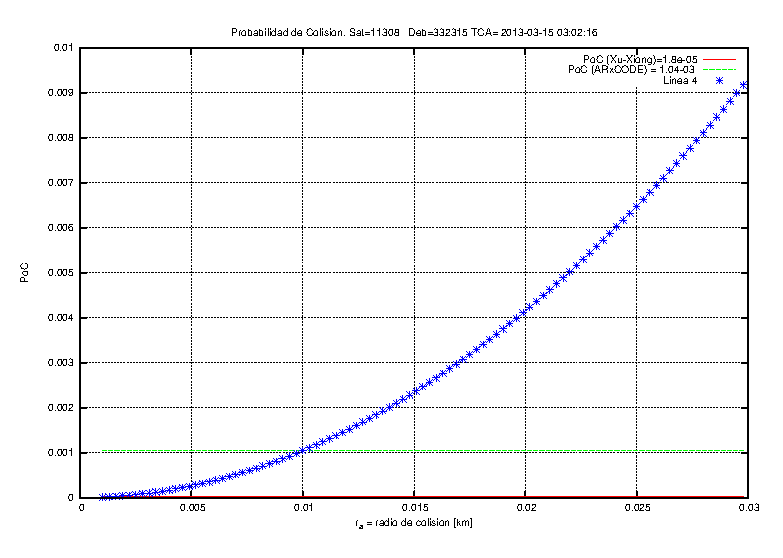
\includegraphics[width=0.6\textwidth]{imagenes/xuxiong4}}
  \caption{An\'alisis de la Probabilidad de Colisi\'on en funci\'on del radio de colisi\'on}
  \label{fig:pocvsraEsc5}
\end{figure}

\newpage
$\ $
\thispagestyle{empty} % para que no se numere esta pagina
\newpage
$\ $
\thispagestyle{empty}
 
\end{document}

